\documentclass[a4paper,11pt,fleqn,dvipsnames,oneside,openright,oldfontcommands]{memoir} 	% Openright aabner kapitler paa hoejresider (openany begge)


%%%%%%%%% Indsat random
%makes it possible to refer to the name of a chapter rather than just the number.
\usepackage{nameref}
\usepackage{pdfpages}
\usepackage{marvosym}
\usepackage{setspace}
\usepackage{graphicx} % For at sætte 2 billeder ved siden af hinanden

%package for writing program code in latex
\usepackage{listings}
%%%%%%%%%%%%%%%%%%%%%%

% ¤¤ Oversaettelse og tegnsaetning ¤¤ %
\usepackage[T1]{fontenc}					% Output-indkodning af tegnsaet (T1)
\usepackage[danish]{babel}					% Dokumentets sprog
\usepackage[utf8]{inputenc}					% Input-indkodning af tegnsaet (UTF8)
\usepackage{ragged2e,anyfontsize}			% Justering af elementer
\usepackage{fixltx2e}						% Retter forskellige fejl i LaTeX-kernen							
				
																							
% ¤¤ Figurer og tabeller (floats) ¤¤ %
\usepackage{graphicx} 						% Haandtering af eksterne billeder (JPG, PNG, EPS, PDF)
%\usepackage{eso-pic}						% Tilfoej billedekommandoer paa hver side
%\usepackage{wrapfig}						% Indsaettelse af figurer omsvoebt af tekst. \begin{wrapfigure}{Placering}{Stoerrelse}
\usepackage{multirow}                		% Fletning af raekker og kolonner (\multicolumn og \multirow)
\usepackage{multicol}         	        	% Muliggoer output i spalter
\usepackage{rotating}						% Rotation af tekst med \begin{sideways}...\end{sideways}
\usepackage{colortbl} 						% Farver i tabeller (fx \columncolor og \rowcolor)
\usepackage{xcolor}							% Definer farver med \definecolor. Se mere: http://en.wikibooks.org/wiki/LaTeX/Colors
\usepackage{flafter}						% Soerger for at floats ikke optraeder i teksten foer deres reference
\let\newfloat\relax 						% Justering mellem float-pakken og memoir
\usepackage{float}							% Muliggoer eksakt placering af floats, f.eks. \begin{figure}[H]
\usepackage{array,booktabs,xcolor,longtable} % kan lave \hdashline i tabellertabe
\usepackage{arydshln}
\usepackage{tabu}

	
	
% ¤¤ Matematik mm. ¤¤
\usepackage{amsmath , amsthm , amsfonts , amssymb, float, stmaryrd} 		% Avancerede matematik-udvidelser
%\usepackage{mathtools}						% Andre matematik- og tegnudvidelser
\usepackage{textcomp}                 		% Symbol-udvidelser (f.eks. promille-tegn med \textperthousand )
\usepackage{rsphrase}						% Kemi-pakke til RS-saetninger, f.eks. \rsphrase{R1}
\usepackage[version=3]{mhchem} 				% Kemi-pakke til flot og let notation af formler, f.eks. \ce{Fe2O3}
\usepackage{siunitx}						% Flot og konsistent praesentation af tal og enheder med \si{enhed} og \SI{tal}{enhed}
\sisetup{output-decimal-marker = {,}}		% Opsaetning af \SI (DE for komma som decimalseparator) 

% ¤¤ Referencer og kilder ¤¤ %
\usepackage[danish]{varioref}				% Muliggoer bl.a. krydshenvisninger med sidetal (\vref)
\usepackage[numbers]{natbib}				% Udvidelse med naturvidenskabelige citationsmodeller
%\usepackage{xr}							% Referencer til eksternt dokument med \externaldocument{<NAVN>}
%\usepackage{glossaries}					% Terminologi- eller symbolliste (se mere i Daleifs Latex-bog)
\usepackage{lastpage}					% Gør det mulig at refere til sidste side 

% ¤¤ Misc. ¤¤ %
\usepackage{listings}						% Placer kildekode i dokumentet med \begin{lstlisting}...\end{lstlisting}
\usepackage{lipsum}							% Dummy text \lipsum[..]
\usepackage[shortlabels]{enumitem}			% Muliggoer enkelt konfiguration af lister
\usepackage{pdfpages}						% Goer det muligt at inkludere pdf-dokumenter med kommandoen \includepdf[pages={x-y}]{fil.pdf}	
\pdfoptionpdfminorversion=6					% Muliggoer inkludering af pdf dokumenter, af version 1.6 og hoejere
\pretolerance=2500 							% Justering af afstand mellem ord (hoejt tal, mindre orddeling og mere luft mellem ord)


% Kommentarer og rettelser med \fxnote. Med 'final' i stedet for 'draft' udloeser hver note en error i den faerdige rapport.
\usepackage[footnote,draft,danish,silent,nomargin]{fixme}		


%%%% CUSTOM SETTINGS %%%%

% ¤¤ Marginer ¤¤ %
\setlrmarginsandblock{3.0cm}{2.5cm}{*}		% \setlrmarginsandblock{Indbinding}{Kant}{Ratio}
\setulmarginsandblock{2.5cm}{3.0cm}{*}		% \setulmarginsandblock{Top}{Bund}{Ratio}
\checkandfixthelayout 						% Oversaetter vaerdier til brug for andre pakker

%	¤¤ Afsnitsformatering ¤¤ %
\setlength{\parindent}{6mm}           		% Stoerrelse af indryk
\setlength{\parskip}{0mm}          			% Afstand mellem afsnit ved brug af double Enter
\linespread{1,1}							% Linie afstand



% ¤¤ Indholdsfortegnelse ¤¤ %
\setsecnumdepth{subsection}		 			% Dybden af nummerede overkrifter (part/chapter/section/subsection)
\maxsecnumdepth{subsection}					% Dokumentklassens graense for nummereringsdybde
\settocdepth{subsection} 					% Dybden af indholdsfortegnelsen

% ¤¤ Lister ¤¤ %
\setlist{
  topsep=0pt,								% Vertikal afstand mellem tekst og listen
  itemsep=-1ex,								% Vertikal afstand mellem items
} 

%hyperlinks in the tabel of contents - comment this out before the report is printed.
\usepackage{hyperref}
\hypersetup{
	bookmarks = true,  % Show 'bookmark'-frame in pdf.
	colorlinks = true, % True = colored links, False = framed links.
	citecolor = black,  % Link color for references.
	linkcolor = black,  % Link color in table of contents.
	urlcolor = black,   % Link color for extern URLs.
}

% ¤¤ Opsaetning af figur- og tabeltekst ¤¤ %
\usepackage{caption}
%\usepackage{subcaption}
\captionnamefont{\small\bfseries\itshape}	% Opsaetning af tekstdelen ('Figur' eller 'Tabel')
\captiontitlefont{\small}					% Opsaetning af nummerering
\captiondelim{. }							% Seperator mellem nummerering og figurtekst
\hangcaption								% Venstrejusterer flere-liniers figurtekst under hinanden
%\captionwidth{0.9\textwidth}					% Bredden af figurteksten
\setlength{\belowcaptionskip}{0pt}			% Afstand under figurteksten
\captionsetup[figure]{labelfont={bf,it},font={it}} % sætter nummer til fed og kursis. Resten til fed + skriften er mindre end resten
\captionsetup[table]{labelfont={bf,it},font={it}} 


% ¤¤ Opsaetning af listings ¤¤ %

\definecolor{commentGreen}{RGB}{34,139,24}
\definecolor{stringPurple}{RGB}{208,76,239}

\lstset{language=Matlab,					% Sprog
	basicstyle=\ttfamily\scriptsize,		% Opsaetning af teksten
	keywords={for,if,while,else,elseif,		% Noegleord at fremhaeve
			  end,break,return,case,
			  switch,function},
	keywordstyle=\color{blue},				% Opsaetning af noegleord
	commentstyle=\color{commentGreen},		% Opsaetning af kommentarer
	stringstyle=\color{stringPurple},		% Opsaetning af strenge
	showstringspaces=false,					% Mellemrum i strenge enten vist eller blanke
	numbers=left, numberstyle=\tiny,		% Linjenumre
	extendedchars=true, 					% Tillader specielle karakterer
	columns=flexible,						% Kolonnejustering
	breaklines, breakatwhitespace=true,		% Bryd lange linjer
}

% ¤¤ Navngivning ¤¤ %
\addto\captionsdanish{
	\renewcommand\appendixname{Bilag}
	\renewcommand\contentsname{Indholdsfortegnelse}	
	\renewcommand\appendixpagename{Bilag}
	\renewcommand\appendixtocname{Bilag}
	\renewcommand\cftchaptername{\chaptername~}				% Skriver "Kapitel" foran kapitlerne i indholdsfortegnelsen
	\renewcommand\cftappendixname{\appendixname~}			% Skriver "Appendiks" foran appendiks i indholdsfortegnelsen
}

% ¤¤ Kapiteludssende ¤¤ %
%\definecolor{numbercolor}{gray}{0.7}		% Definerer en farve til brug til kapiteludseende
%\newif\ifchapternonum

\makechapterstyle{AAU}
{
	% Afstand mellem sidehovedet og kapitel+tal+kapitelnavnet defineres til:
	\setlength{\beforechapskip}{0cm}

	% Afstanden mellem kapitelnavnet og body-teksten defineres til:
	\setlength{\afterchapskip}{2cm}

	% Typografiopsætningen til kapitel+tal defineres til:
	\renewcommand\chapnamefont{\sffamily\bfseries\LARGE\raggedright}
	
	% Typografiopsætningen til kapitel+tal defineres til:
	\renewcommand\chaptitlefont{\sffamily\bfseries\huge\color[cmyk]{1.00,0.38,0.00,0.64}}

	% Forårsager, at der til kapitlet også tilføjes dets respektive tal:
	\renewcommand\chapternamenum{}
	\renewcommand\printchapternum
	{
		\makebox[0pt][l]
		{
			\color[cmyk]{1.00,0.38,0.00,0.64}
			\hspace{0.1cm}
			\resizebox{!}{1cm}{\chapnamefont\bfseries\sffamily\thechapter}
		}
	}
	
	% Definitionen af linjenstykket mellem ``Kapitel #'' samt ``kapitelnavnet'':
			\renewcommand\afterchaptertitle{\par\hspace{1.5cm}\hrule height 1pt\vskip\midchapskip}
}

% Aktivering af selve kapitellayoutet med dét navn, som definerer kapitellayoutet (ses fra tidligere):
\chapterstyle{AAU}

%\makechapterstyle{jenor}{					% Definerer kapiteludseende frem til ...
%  \renewcommand\beforechapskip{0pt}
%  \renewcommand\printchaptername{}
%  \renewcommand\printchapternum{}
% % \renewcommand\printchapternonum{\chapternonumtrue}
%  \renewcommand\chaptitlefont{\fontfamily{pbk}\fontseries{db}\fontshape{n}\fontsize{20}{25}\selectfont\raggedright}
%  \renewcommand\chapnumfont{\fontfamily{pbk}\fontseries{m}\fontshape{n}\fontsize{1in}{0in}\selectfont\color{numbercolor}}
% \renewcommand\printchaptertitle[1]{
%    \noindent
%    \ifchapternum
%     \begin{tabularx}{\textwidth}{XI}
%	{\let\\\newline\chaptitlefont ##1\par}     
%    \end{tabularx}
%    \par\vskip-2.5mm\hrule
%    \else
%    \begin{tabularx}{\textwidth}{X}
%      {\parbox[b]{\linewidth}{\chaptitlefont ##1}} & \raisebox{-15pt}{\chapnumfont \thechapter}
%    \end{tabularx}
%    \par\vskip2mm\hrule
%    \fi
%  }
%}											% ... her
%
%\chapterstyle{jenor}						% Valg af kapiteludseende - Google 'memoir chapter styles' for alternativer

% ¤¤ Sidehoved ¤¤ %

\makepagestyle{AAU}							% Definerer sidehoved og sidefod udseende frem til ...
\makepsmarks{AAU}{%
	\createmark{chapter}{left}{shownumber}{}{. \ }
	\createmark{section}{right}{shownumber}{}{. \ }
	\createplainmark{toc}{both}{\contentsname}
	\createplainmark{lof}{both}{\listfigurename}
	\createplainmark{lot}{both}{\listtablename}
	\createplainmark{bib}{both}{\bibname}
	\createplainmark{index}{both}{\indexname}
	\createplainmark{glossary}{both}{\glossaryname}
}
\nouppercaseheads											% Ingen Caps oenskes

\makeoddhead{AAU}{Gruppe 16gr5404}{}{\leftmark}				% Definerer lige siders sidehoved (\makeevenhead{Navn}{Venstre}{Center}{Hoejre})
\makeevenhead{AAU}{\rightmark}{}{Aalborg Universitet}		% Definerer ulige siders sidehoved (\makeoddhead{Navn}{Venstre}{Center}{Hoejre})
\makeevenfoot{AAU}{Side \thepage\ af \pageref{LastPage}}{}{}							% Definerer lige siders sidefod (\makeevenfoot{Navn}{Venstre}{Center}{Hoejre})
\makeoddfoot{AAU}{}{}{Side \thepage\ af \pageref{LastPage}}								% Definerer ulige siders sidefod (\makeoddfoot{Navn}{Venstre}{Center}{Hoejre})
\makeheadrule{AAU}{\textwidth}{0.5pt}						% Tilfoejer en streg under sidehovedets indhold
\makefootrule{AAU}{\textwidth}{0.5pt}{1mm}					% Tilfoejer en streg under sidefodens indhold

\copypagestyle{AAUchap}{AAU}								% Sidehoved for kapitelsider defineres som standardsider, men med blank sidehoved
\makeoddhead{AAUchap}{}{}{}
\makeevenhead{AAUchap}{}{}{}
\makeheadrule{AAUchap}{\textwidth}{0pt}
\aliaspagestyle{chapter}{AAUchap}							% Den ny style vaelges til at gaelde for chapters
															% ... her
															
\pagestyle{AAU}												% Valg af sidehoved og sidefod


%%%% CUSTOM COMMANDS %%%%

% ¤¤ Billede hack ¤¤ %
\newcommand{\figur}[4]{
		\begin{figure}[H] \centering
			\includegraphics[width=#1\textwidth]{billeder/#2}
			\caption{#3}\label{#4}
		\end{figure} 
}

% ¤¤ Specielle tegn ¤¤ %
\newcommand{\decC}{^{\circ}\text{C}}
\newcommand{\dec}{^{\circ}}
\newcommand{\m}{\cdot}


%%%% ORDDELING %%%%

\hyphenation{}

%%%%Fra engelsk til dansk i \autoref{•} %%%%
\renewcommand{\figureautorefname}{figur}
\renewcommand{\sectionautorefname}{afsnit}
\renewcommand{\subsectionautorefname}{afsnit}
\renewcommand{\subsubsectionautorefname}{afsnit}
\renewcommand{\tableautorefname}{tabel}
\renewcommand{\appendixautorefname}{bilag}
\renewcommand{\equationautorefname}{ligning}
\renewcommand{\itemautorefname}{punkt}
\renewcommand{\chapterautorefname}{kapitel}
%Figure references:
\newcommand{\figref}[1]{figur \ref{#1}}

%Figure references after full stop/period:
\newcommand{\Figref}[1]{Figur \ref{#1}}

%Table references:
\newcommand{\tabref}[1]{tabel \ref{#1}}

%Table references after full stop/period:
\newcommand{\Tabref}[1]{Tabel \ref{#1}}

%Section references:
\newcommand{\secref}[1]{afsnit \ref{#1} på side \pageref{#1}}

%Section references:
\newcommand{\Secref}[1]{Afsnit \ref{#1} på side \pageref{#1}}

%Appendix references:
\newcommand{\appref}[1]{appendiks \ref{#1} på side \pageref{#1}}

%Appendix references:
\newcommand{\Appref}[1]{Appendiks \ref{#1} på side \pageref{#1}}

%chapter references: 
\newcommand{\chapref}[1]{kapitel \ref{#1} på side \pageref{#1}}

%chapter references: 
\newcommand{\Chapref}[1]{Kapitel \ref{#1} på side \pageref{#1}}

%Units:
%\newcommand{\unit}[1]{&& \left[\si{#1}\right]}

%Text:
\newcommand{\tx}[1]{\text{#1}}

%Equation references:
%1 equation:
\renewcommand{\eqref}[1]{ligning (\ref{#1})}
%2 equations:
%\newcommand{\eqrefTwo}[2]{ligning (\ref{#1})} and \textbf{(\ref{#2})}
%%3 equations:
%\newcommand{\eqrefThree}[3]{ligning (\ref{#1})}, \textbf{(\ref{#2})} and \textbf{(\ref{#3})}
%%4 equations:
%\newcommand{\eqrefFour}[4]{ligning (\ref{#1})}, \textbf{(\ref{#2})}, \textbf{(\ref{#3})} and \textbf{(\ref{#4})}
%%5 equations:
%\newcommand{\eqrefFive}[5]{ligning (\ref{#1})}, \textbf{(\ref{#2})}, \textbf{(\ref{#3})}, \textbf{(\ref{#4})} and \textbf{(\ref{#5})}
%%5 equations:
%\newcommand{\eqrefSix}[6]{ligning (\ref{#1})}, \textbf{(\ref{#2})}, \textbf{(\ref{#3})}, \textbf{(\ref{#4})}, \textbf{(\ref{#5})} and \textbf{(\ref{#6})}
%%5 equations:
%\newcommand{\eqrefSeven}[7]{ligning (\ref{#1})}, \textbf{(\ref{#2})}, \textbf{(\ref{#3})}, \textbf{(\ref{#4})}, \textbf{(\ref{#5})}, \textbf{(\ref{#6})} and \textbf{(\ref{#7})}
%
%%Equation references after full stop/period:
%%1 equation:
%\newcommand{\Eqref}[1]{Ligning (\ref{#1})}
%%2 equations:
%\newcommand{\EqrefTwo}[2]{Ligning (\ref{#1})} and \textbf{(\ref{#2})}
%%3 equations:
%\newcommand{\EqrefThree}[3]{Ligning (\ref{#1})}, \textbf{(\ref{#2})} and \textbf{(\ref{#3})}
%%4 equations:
%\newcommand{\EqrefFour}[4]{Ligning (\ref{#1})}, \textbf{(\ref{#2})}, \textbf{(\ref{#3})} and \textbf{(\ref{#4})}
%%5 equations:
%\newcommand{\EqrefFive}[5]{Ligning (\ref{#1})}, \textbf{(\ref{#2})}, \textbf{(\ref{#3})}, \textbf{(\ref{#4})} and \textbf{(\ref{#5})}
%%5 equations:
%\newcommand{\EqrefSix}[6]{Ligning (\ref{#1})}, \textbf{(\ref{#2})}, \textbf{(\ref{#3})}, \textbf{(\ref{#4})}, \textbf{(\ref{#5})} and \textbf{(\ref{#6})}
%%5 equations:
%\newcommand{\EqrefSeven}[7]{Ligning (\ref{#1})}, \textbf{(\ref{#2})}, \textbf{(\ref{#3})}, \textbf{(\ref{#4})}, \textbf{(\ref{#5})}, \textbf{(\ref{#6})} and \textbf{(\ref{#7})}
\raggedbottom % Soerger for at LaTeX ikke "straekker" teksten

%-------------DEF. ALIAS--------------------
\defcitealias{hasse2012}{'Teknologiforståelse - på skoler og hospitaler'}
\defcitealias{kaewkannate2016}{'A comparison of wearable fitness devices'} 
\defcitealias{mercer2016}{'Acceptance of Commercially Available Wearable Activity Trackers Among Adults Over 50 and With Chronic Illness: A Mixed-Methods Evaluation'}
\defcitealias{rapp2016}{'Personal informatics for everyday life: How users without prior self-tracking experience engage with personal data'}
\defcitealias{pedersen2011}{'Fysisk Aktivitet - Håndbog om forebyggelse og behandling'}
\defcitealias{evenson2015}{'Systematic review of the validity and reliability of consumer-wearable activity trackers'}
\defcitealias{galper2006}{'Inverse Association between Physical Inactivity and Mental Health in Men and Women'}
\defcitealias{munck2007}{'Projektgruppen for hypertensionsaudit ved Anders Munck'}



%-------------Formaliteter-------------------
\begin{document}

\frontmatter	 
\clearpage
\thispagestyle{empty}

\begin{figure}[H]
	\raggedleft
		
\includegraphics[width=0.2\textwidth]{figures/aaulogo-da.png}
\end{figure} 
\vspace*{\fill} 
\begin{center}
\begin{Huge}
\textbf{Registrering og objektivisering af fysisk aktivitetsniveau hos kronikere i almen praksis via aktivitetsarmbånd}\\
\vspace{5 mm}
5. semesterprojekt - Efterår $2016$\\
\vspace{3 mm}
\end{Huge}
{\Large Gruppe $16$gr$5404$}
\begin{figure}[H]
	\centering
	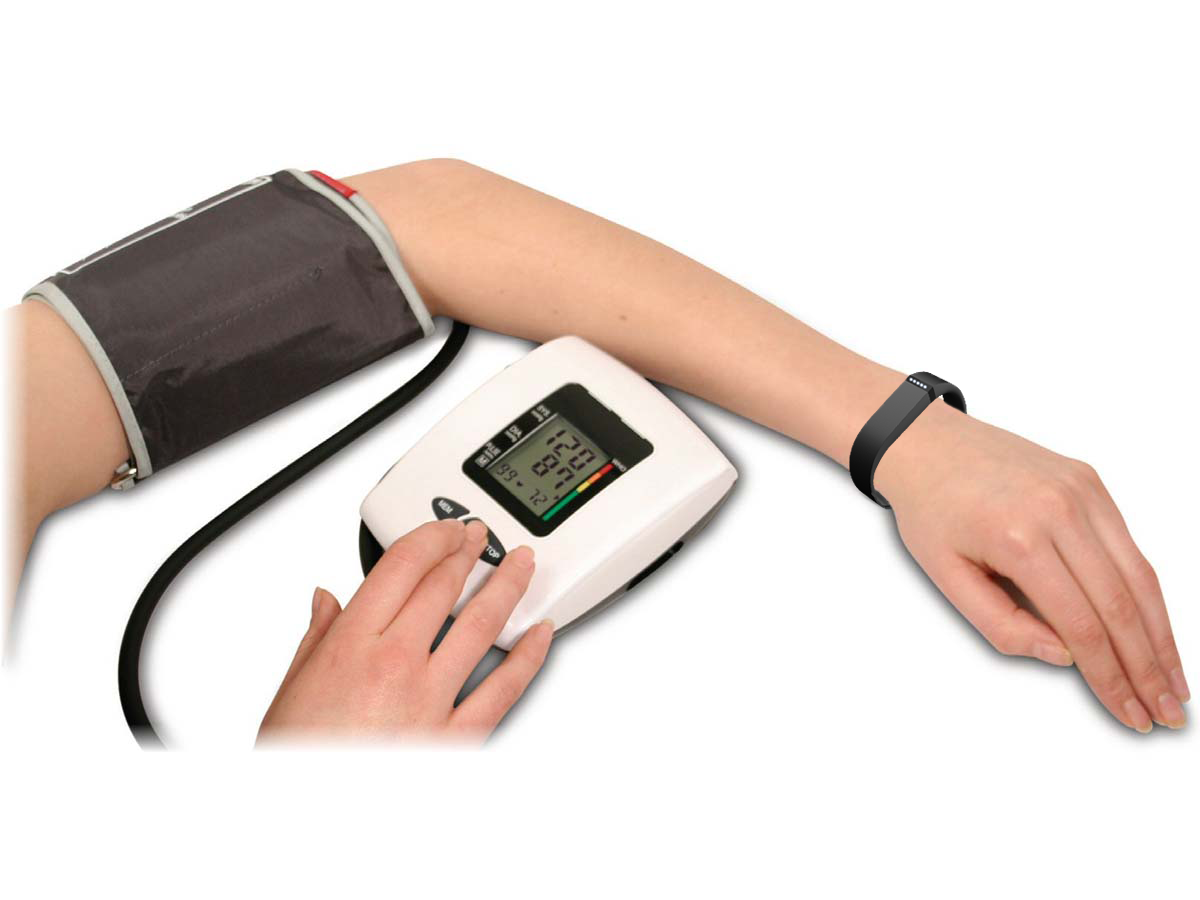
\includegraphics[width=0.8\textwidth]{figures/forside}
\end{figure}	
\end{center}
\vspace*{\fill}

\begin{center}
\line(1,0){400}
\end{center}
%\begin{document} 
\thispagestyle{empty}
%\begin{titlepage}
\begin{nopagebreak}
{\samepage 

\begin{tabular}{r}
\parbox{\textwidth}{ 
 {
\includegraphics[height=2.5cm]{figures/aaulogo-da.png}}
\hfill \hspace{2cm} \parbox{8cm}
{\begin{tabular}{l} %4.90
{\small \textbf{5. semester}}\\
{\small \textbf{School of Medicine and Health}}\\
%{\small \textbf{\textcolor{MidnightBlue}{}}}\\ 
{\small \textbf{Sundhedsteknologi}}\\
{\small Fredrik Bajers Vej $7$A} \\
{\small $9220$ Aalborg} \\
%{\small \textcolor{NavyBlue}{\emph{http://www.smh.aau.dk/}}}
\end{tabular}}}
\end{tabular}

\hspace{-1.5cm}\begin{tabular}{cc}
\parbox{7cm}{
\begin{description}

\item {Titel:}

Registrering og objektivisering af fysisk aktivitetsniveau hos kronikere i almen praksis via aktivitetsarmbånd\\

\item {Tema:} 


Klinisk teknologi\\

\end{description}

\parbox{8cm}{

\begin{description}
\item {Projektperiode:}\\
   Efteråret $2016$\\
   $02/09/2016$ - $19/12/2016$\\
   
\item {Projektgruppe:}\\
  $16$gr$5404$\\
  
\item {Medvirkende:}\\
Birgithe Kleemann Rasmussen\\
Mads Kristensen\\
Signe Hejgaard Kristoffersen\\
Simon Bruun\\
Suado Ali Haji Diriyi\\
Toby Steven Waterstone

\hspace{2cm}
\item {Vejledere:}\\
Ole Hejlesen, Morten Sig Ager Jensen \\
og Mads Nibe Stausholm\\
\end{description}

}\\
\begin{description}
\item {Sider: ??} \\
%\item {Appendikser: ??}\\
\hspace{1.5cm}
%\item {Afsluttet: $27/05/2016$}
\end{description}
\vfill } &
\parbox{7cm}{
  \vspace{.15cm}
  \hfill 
  \begin{tabular}{l}
  {Synopsis:}\bigskip \\
  \fbox{
    \parbox{9cm}{\bigskip
     {\vfill{\small Denne rapport belyser idéen af at anvende et aktivitetsarmbånd til monitorering af hypertensive patienters aktivitetsniveau. 
Hypertension er en folkesygdom, og i Danmark er det vurderet, at 20 \% har sygdommen. Disse patienter anbefales fysisk aktivitet som en del af behandlingen, da dette resulterer i et reduceret blodtryk, hvorpå risikoen for følgesygdomme og medicinering ligeledes kan reduceres eller udskydes. 
Formålet har således været at undersøge et udvalgt aktivitetsarmbånd, Fitbit Flex, og vurdere, om dette hensigtsmæssigt kan anvendes i behandlings- og/eller udredningsforløb af hypertension. 
Den registrerede aktivitet vil give læger og andet relevant sundhedsfagligt personale indblik i patienters aktivitetsniveau, hvorved en korrekt rådgivning kan gives til patienten. 

Vurderingen af Fitbit Flex som registrering- og objektiviseringsmetode er fortaget med udgangspunkt i metoden for en medicinsk teknologi vurdering.  

På baggrund af flere studier er det vist at aktivitetsarmbånd har potentialet til at motivere personer til at være mere fysisk aktive, hvilket vil kunne medføre en gavnlig effekt på hypertensive patienters tilstand. Yderligere ved at data gemmes ved brug af en applikation tilhørende aktivitetsarmbåndet, muliggøres en objektiv monitorering af bæren af armbåndet, hvilket vil kunne give grundlag og viden for lægen, om vejledning og anbefalinger om hvordan patientens behandlingsforløb kan struktureres ved fremtidig behandling.

Implementeringen af aktivitetsarmbånd vil indledningsvist kræve resourser i den primære sundhedssektor, men såfremt aktivitetsarmbånd viser sig effektivt for behandlingen af hypertensive patienter, vil resultatet kunne afspejle sig i et overordnet lettere behandlingsforløb.
     \bigskip}}
     }}
   \end{tabular}}
\end{tabular}} \hspace{-1.5cm}%\vspace{1.0cm}

\vfill
{\footnotesize\itshape \noindent Offentliggørelse af rapportens indhold, med kildeangivelse, må kun ske efter aftale med forfatterne.}
\\
\end{nopagebreak}
%\end{titlepage}
%\end{document}
\chapter{Forord}
Skriv forord her.... 


\section*{Læsevejledning}
Denne rapport består af et initierende problem, en problemanalyse, en problemformulering, MTV-spørgsmål og -analyser samt en syntese af disse analyser, der gerne skal besvare problemformuleringen. 

Det initiernede problem og problemanalysen belyser og analyserer projektets problemstillinger og leder frem til en problemformulering igennem en problemafgrænsning. MTV-spørgsmålene og -analyserne beskæftiger sig med de fire MTV-elementer; patient, teknologi, organisation og økonomi. Syntesen dækker over en diskussion af MTV-analyserne, en konklusion på problemformuleringen samt en perspektivering til valgte teknologi i projektet. 


\subsection*{Kildeangivelse}
I denne rapport bliver kilder angivet ved Vancouver-metoden, hvor kilden henvises til som et nummer i kantede parenteser. Information omkring kilden findes i litteraturlisten.


%Teknologiafsnittet vil beskrive den valgte teknologi, og hvilke variationer af teknologien der eksistere i dag. En sammenligning af variationerne vil blive fortaget, med henblik på at fremhæve fordele og ulemper. Yderligere vil teknologien også blive sammenlignet med de nuværende løsningsmuligheder der anvendes i dag, for at se hvordan de adskiller sig fra hinanden.  

%Patientafsnittet i MTV’en undersøges den afgrænsede patientgruppe nærmere i forhold til teknologien. Der undersøges blandt andet om teknologien vil have en betydelig påvirkning på patienternes hverdag, og om den kan forbedre deres livskvalitet. Yderligere undersøges om eventuelle etiske problemstillinger forekommer ved anvendelse af teknologien.

%Den organisatoriske analyse vil hovedsageligt behandle ændringer i interaktionen mellem patienter og sundhedspersonale, samt det organisatoriske aspekt i forhold til samarbejdet mellem forskellige sundhedsinstitutioner: primær og sekundær sundhedssektor.

%Det økonomiske aspekt blive undersøgt, med udgangspunkt i at finde frem til omkostningerne relateret til de teknologiske løsninger, som er undersøgt i teknologianalysen. Dette omhandler eventuelle besparelser eller ekstraudgifter, der kan forekomme ved implementering af den nye teknologi.







%\section{Metode} \label{metode}

%Denne medicinske teknologivurdering (MTV) vil afvige fra opbygningen beskrevet i MTV-håndbogen, som følge af projektet samtidig indeholder elementer fra problembaseret læring (PBL). Som et resultat af blandingen, tages der udgangspunkt i en medicinsk problemstilling, som analyseres for at udarbejde en problemformulering. Analysen i forbindelse med PBL-tilgangen vil desuden indeholde MTV-elementer såsom etik, målgruppe og interessentanalyse.

%Efterfølgende vil problemformuleringen skabe grundlag for at arbejde videre med MTV-håndbogens elementer. Her vil de fire områder, teknologi, patient, organisation og økonomi, blive anvendt til at stille mere konkrete spørgsmål. Fremgangsmåden betyder at der vil være tale om en problem- og teknologiorienteret MTV, da der søges at finde en løsning på et medicinsk problem gennem en vurdering af, hvorvidt en ny teknologi vil afhjælpe de problemer, der er ved den nuværende løsningsmetode.

%Teknologiafsnittet vil indeholde en beskrivelse af egenskaberne for den nuværende teknologi, samt en undersøgelse af den alternative behandlingsmetode, der ligger til grunde for MTV'en. Efter den nuværende og den alternative teknologi er beskrevet, vil disse blive sammenholdt, med henblik på at finde fordele og ulemper ved de to løsningsforslag.

%I forbindelse med patientafsnittet i MTV-modellen afgrænses patientgruppen, med henblik på at gøre problemet konkret, hvorved målgruppen for teknologien kan undersøges nærmere. Der undersøges blandt andet hvorvidt teknologien vil have en betydelig påvirkning på patienternes hverdag og om der skal tages højde for etiske problemstillinger.

%Den organisatoriske analyse vil hovedsageligt behandle ændringer i interaktionen mellem patienter og sundhedspersonale, samt det organisatoriske aspekt i forhold til samarbejdet mellem forskellige sundhedsinstitutioner.

%Som et led i MTV'en vil det økonomiske aspekt blive undersøgt med udgangspunkt i, at finde frem til omkostningerne relateret til de teknologiske løsninger, som er undersøgt i teknologianalysen. Her undersøges desuden hvilke besparelser eller ekstraudgifter, der kan forekomme ved implementering af den nye teknologi.

%Analysen af de fire MTV-elementer vil dernæst blive anvendt i syntesen, der indeholder en diskussion med udgangspunkt i fordele og ulemper ved både den nuværende og den undersøgte teknologi. Herigennem vil PBL-metoden også komme til udtryk, i og med syntesen leder frem til en konklusion, som vil besvare den indledende problemformulering. 


\section*{Ordliste}
\begin{itemize}
\item PLO:  Praktiserende Lægers Organisation
\item RLTN: Regionernes Lønnings- og TakstNævn
\item Applikation: Et program, der anvendes under et operativsystem, som bruges til at løse specifikke opgaver
\item MEMS: Micro Electro-Mechanical System
\end{itemize}

\clearpage

%-----------Indholdsfortegnelse-------------
\phantomsection									
\pdfbookmark[0]{Indholdsfortegnelse}{indhold}	
\tableofcontents*								

\mainmatter

\part{ Problemstilling}

%-------------Indledning-----------------
\chapter{Indledning}
I Danmark dør 4.500 mennesker årligt som følge af fysisk inaktivitet, hvor fysisk inaktivitet jf. Sundhedsstyrelsen defineres som værende mindre end 2,5 times fysisk aktivitet per uge. \citep{aagaard2014} Fysisk inaktivitet har konsekvenser for kroppens fysiologiske tilstand og helbred, da det er en risikofaktor for psykiske sygdomme, livsstilssygdomme såsom type-2 diabetes eller visse hjertekarsygdomme, samt en for tidlig død for blandt andet patienter med type-2 diabetes og hypertension. \citep{motionsraad2007} 

Fysisk inaktivitet påvirker blandt andet kroppens kredsløb, muskler, knogler og metabolisme, hvilket vil resultere i en reduceret arbejdskapacitet for kroppen og eventuelt funktionstab. På længere sigt kan fysisk inaktivitet øge risikoen for tidlig død, da det er dokumenteret, at regelmæssig fysisk aktivitet nedsætter risikoen for tidlig død. \citep{motionsraad2007}

Sundhedsstyrelsen anbefaler, at voksne bør være aktive minimum 30 minutter dagligt med moderat intensitet, hvilket forstås som 40-59 $\%$ af den maksimale iltoptagelse pågældende eller motion, hvor man bliver lettere forpustet, men hvor det er muligt at føre en samtale.
Aktivitet i dagligdagen er nødvendigt i alle aldersgrupper, og anbefalingerne er specificeret til de enkelte aldersgrupper. Herunder er det understreget, at børn skal være fysisk aktiv minimum 60 minutter dagligt, samt at ældre skal lave udstrækningsøvelser. \citep{pedersen2011}

Fysisk aktivitet kan anvendes til at forebygge flere sygdomme, og en struktureret fysisk træning kan yderligere benyttes som en del af en behandling eller til at forebygge en eventuel videreudvikling af flere sygdomme. \citep{motionsraad2007} Dette kræver, at der fokuseres på fysisk aktivitet under behandling af patienter, hvor dette kan have en positiv effekt.

\textit{Telemedicin kan benyttes som en del af denne behandling, hvor hjemmemonitorering af fysisk aktivitet er en mulighed. Aktivitetsniveauet kan derved registreres af patienten selv, og dette kan efterfølgende evalueres af egen læge eller andet sundhedsfagligt personale. På denne måde kan patient og sundhedsselktoren spare besøg og transporter ved brug af opfølgning på indberettet data. \citep{medcom2010} - skal dette med? mere problemanalyse?}


%Dette projekt tager udgangspunkt i formålet at registrere fysisk aktivitetsniveau hos kronikere i almen praksis. Der vil hertil blive anvendt en medicinsk teknologivurdering håndbog, hvor fire elementer vil blive analyseret med formål at vurdere... - er dette relevant?



%[1]https://www.sundhed.dk/borger/sygdomme-a-aa/sundhedsoplysning/idraet-og-motion/fysisk-inaktivitet/ 

%[2]http://sundhedsstyrelsen.dk/publ/MER/2007/FYSISK_INAKTIVITET-KONSEKVENSER_OG_SAMMENHAENGE2007.PDF 

%[3]http://medcom.dk/media/1462/udredning-om-telemedicin-april-2010.pdf 

\section{Initierende problem}
Hvordan holdes styr på aktivitetsniveau ved patienter? 

Hvorpå er det muligt at kontrollere et givent aktivitetsniveau ved patienter? 

%-------------Problemanalyse----------------
\chapter{Problemanalyse}
\section{Fysisk aktivitet}\label{sec:prob_fysaktiv}

I det danske sundhedsvæsen defineres fysisk aktivitet som værende en aktivitet, der forhøjer energiomsætningen. Dette betyder, at alt fra indkøb og gåture til målrettet fysisk træning, kan defineres som værende fysisk aktivitet \citep{motionsraad2007, terkelsen2015}.

Som nævnt i \autoref{sec:indledning} anbefaler Sundhedsstyrelsen et aktivitetsniveau på minimum 30 minutters motion af moderat intensitet hver dag. I forbindelse med dette, er moderat intensitet defineret som $40-59~\%$ af maksimal iltoptagelse, $64-74~\%$ af makspuls eller som et aktivitetsniveau, der gør patienten lettere forpustet, uden at forhindre muligheden for samtale \citep{motionsraad2007}.
Ud over anbefalingerne til voksne er det understreget, at børn skal være fysisk aktive minimum 60 minutter dagligt \citep{pedersen2011}. 

\section{Effekter af fysisk aktivitet}
Fysisk aktivitet kan påvirke kroppens fysiologiske tilstand på mange måder, herunder kan det i forskellige grader forbedre blandt andet immunforsvar, lungefunktion, blodtryk, muskelstyrke- og udholdenhed samt kroppens bevægelighed og vægt. Desuden bemærkes en forbedring af glukosetransportering til muskelcellerne, hvilket medfører, at insulinniveauet er lavere hos folk, der udfører regelmæssig fysisk aktivitet. \citep{andersen2001, martini2015}. Dette betyder, at forskellige sygdomme, der relateres til nogle af de nævnte fysiologiske funktioner, kan påvirkes ved fysisk aktivitet.

Flere studier indikerer, at fysisk aktivitet kan have en forebyggende effekt på forskellige folke- og livsstilssygdomme \citep{warburton2010}. Nogle af disse folke- og livsstilssygdomme er muskel-og skeletlidelser, stress, samt en række kredsløbssygdomme såsom hjertekarsygdomme, hypertension, overvægt og type-2 diabetes. Foruden disse forebygger fysisk aktivitet også nogle kræfttyper, herunder tyktarmskræft og brystkræft. De nævnte lidelser er gældende for alle aldersgrupper, og foruden disse er særlige effekter af fysisk aktivitet gældende for enkelte aldersgrupper. Eksempelvis udskyder eller reducerer den ældre del af befolkningen, der udfører fysisk aktivitet, den aldersrelaterede reduktion i funktionsevne, som forventes med alderen. Risikoen for apopleksi og islæmisk hjertesygdom nedsættes samtidig som følge af fysisk aktivitet hos ældre \citep{pedersen2011,
warburton2010}. 

Fysisk aktivitet kan ligeledes have en psykisk effekt. Det kan blandt andet forebygge psykiske lidelser som depression, angst og demens cite{pedersen2011}. De psykologiske påvirkninger kan skyldes, at endorfinkoncentrationen i blodet øges ved fysisk aktivitet. Endorfiner virker som kroppens egen produktion af morfinlignende stoffer \citep{kessing2016}. Større overskud, mere selvtillid samt bedre social trivsel er også ofte en effekt af fysisk aktivitet \citep{sundhedsstyrelsen2006}. 

Mange af de nævnte sygdomme, både de fysiske og psykiske, kan desuden behandles med fysisk aktivitet. Fysisk aktivitet kan være den primære behandlingsmetode eller det kan være en del af behandlingen, eksempelvis i samspil med medicinsk behandling. Type-2 diabetikere og hypertensive er eksempler på patientgrupper, hvor fysisk aktivitet ofte er en del af behandlingsforløbet, hvor graden af lidelsen har betydning for om fysisk aktivitet og andre livsstilsændringer er den primære behandling eller om behandlingen skal kombineres med medicin. Ved behandling af visse sygdomme eller tilstande skal der tages hensyn til, hvilken form for fysisk aktivitet, der egner sig til forskellige patientgrupper, da det ellers kan have en skadende effekt. Nogle af disse patientgrupper er eksempelvis artrosepatienter, der specielt skal undgå overbelastning af led. Det kan også være gravide, som skal undgå fysisk aktivitet, hvor uventede stød kan forekomme \citep{andersen2001, pedersen2011}.

\section{Fysisk inaktivitet}

Definitionen af både fysisk aktivitet og inaktivitet varierer afhængigt af, hvilken sundhedsinstans, der har opstillet definitionen. Center for Disease Control and Prevention (CDC) i USA anbefaler mindst $30$ minutters moderat arbejdsintensitet, såsom rask gang eller havearbejde, $5$ dage om ugen, eller $20$ minutters aktivitet af høj intensitet $3$ dage om ugen \citep{motionsraad2007,christensen2012}.
Samtidig definerer CDC forskellige niveauer af fysisk inaktivitet, hvoraf disse er henholdsvis anbefalet fysisk aktivitet, utilstrækkelig fysisk aktivitet, inaktivitet samt inaktivitet i fritiden. Heraf svarer utilstrækkelig fysisk aktivitet til et aktivitetsniveau ved moderat eller høj intensitet, der ligger under det anbefalede aktivitetsniveau, hvor der dog udføres mere end $10$ minutters fysisk aktivitet ugentligt. Ved niveuaet inaktivitet udføres der mindre end $10$ minutters ugentligt fysisk aktivitet ved moderat eller høj intensitet. Der er desuden ikke rapporteret fysisk aktivitet i den foregående måned i fritiden i niveauet inaktivitet  \citep{motionsraad2007,christensen2012}.
%Samtidig definerer CDC forskellige niveauer af fysisk inaktivitet, hvor det første er utilstrækkelig fysisk aktivitet med mellem $10$ minutters aktivitet om ugen til det anbefalede niveau. Under dette niveau er inaktivitet, der defineres som mindre end $10$ minutters fysisk aktivitet om ugen \citep{motionsraad2007,christensen2012}.

Sundheds- og sygelighedsundersøgelsen af \citeauthor{christensen2012} definerer fysisk inaktivitet ud fra ét enkelt spørgsmål vedrørende den mest passende beskrivelse af patientens fritidsaktiviteter igennem det sidste år. Svarmulighederne til dette spørgsmål er hård træning flere gange om ugen, motionsidræt eller tungt arbejde mindst fire timer om ugen, lettere motion mindst fire timer om ugen samt stillesiddende aktivitet. Besvarer patienten spørgsmålet med "Læser, ser fjernsyn eller har anden stillesiddende beskæftigelse", kategoriseres patienten som værende fysisk inaktiv \citep{motionsraad2007,christensen2012}.

Både Sundhedsstyrelsen og World Health Organization (WHO) definerer fysisk inaktivitet, som værende mindre end $2,5$ timers fysisk aktivitet om ugen. Af denne grund vælges det i projektet, at tage udgangspunkt i Sundhedsstyrelsen og WHO's definition af fysisk inaktivitet, når begrebet omtales senere i projektet \citep{motionsraad2007}.
\subsection{Årsager til fysisk inaktivitet}
Fysisk inaktivitet er forårsaget af forskellige faktorer, som eksempelvis livsstil og den teknologiske udvikling gennem tiden. Manglende tid, motivation og interesse er dog en af de overordnede årsager til fysisk inaktivitet \citep{ottesen2005}.  

\subsubsection{Teknologiske faktorer}  
Siden den industrielle revolution er teknologi et område, der er i konstant udvikling, og anvendes blandt andet som skåneredskab for at aflaste den almene arbejder for fysisk hårdt arbejde, samt invaliditet heraf \citep{hallal2012}. 
Ligeledes har udviklingen ledt til en reduktion i mængden af fysisk aktivitet krævet for at komme igennem hverdagen. Dette betyder blandt andet let adgang til mad og drikkevarer, som ikke kræver stor energiomsætning for at skaffe. \citep{hallal2012, motionsraad2007}.  Transport foregår ofte med bil eller bus, og teknologier som tv, trådløs kommunikation, internet og lignende bidrager til fysisk inaktivitet \citep{hallal2012}.  

\subsubsection{Kropslige faktorer}
Alder er blandt disse faktorer, hvor det på verdensplan ses, at fysisk inaktivitet stiger i takt med alderen \citep{guthold2008}. 
Årsagen til dette hos danske ældre er, at de ikke føler det nødvendige overskud, til fysisk aktivitet efter de stadig sværere gøremål i hverdagen. 
Overvægtige oplever frygt og manglende motivation ved fysisk aktivitet, idet de forbinder det med ubehag og usikkerhed i hvad deres krop reelt kan holde til \citep{ottesen2005}. 
Psykiske forhindringer for fysisk aktivitet fremtræder som flovhed for at vise sig frem i et træningscenter, samt at individer ikke føler de passer ind med omgivelserne ved aktivitet. 
Dertil forekommer ligeledes manglende motivation og/eller interresse \citep{ottesen2005}.

\subsubsection{Økonomiske faktorer}
Fysisk inaktivitet kan også være forårsaget af økonomiske årsager, hvor eksempelvis betaling for medlemskab af et træningscenter vil sætte en begrænsning for nogle personer. Yderligere forbindes fysisk aktivitet med noget, der er for tidskrævende eller besværligt at få plads til i hverdagenen \citep{ottesen2005}.
\section{Følger af fysisk inaktivitet}
'Der mangler lige lidt tekst her så der ikke er overskrift på overskrift'

\subsection{Fysiske følger}
Der foregår en lang række fysiologiske processer i kroppen, alle disse er i høj grad tilpasset til det miljø, vi lever i på jorden. 
Tyngdekraften udgør en belastning på vores legeme, som sammen med de bevægelser vi udfører, når vi er fysisk aktive, skaber et stress på kroppen. 
Hvis kroppen ikke udsættes for dette stress, tilpasser kroppen sig ved, at nedgradere de biologiske mekanismer og processer. Omvendt forstærkes de når vi stimulerer dem. 
Blandt disse biologiske mekanismer og processer kan nævnes kredsløbet, stofskiftet, muskelvækst og knoglevækst \citep{motionsraad2007}.

\subsection{Kredsløb}
Kredsløbet er en af de mekanismer som påvirkes relativt hurtigt ved fysisk inaktivitet. 
Et studie af \citeauthor{Convertino1995}, som foregik over 4 uger, har påvist et fald i aerob kapacitet (VO2max), som angiver den maksimale iltoptagelse i kroppen under fysisk arbejde i forhold til tid, med 5 til 6 \% pr. uge. 
Personerne som blev testet var både kvinder og mænd i aldersgruppen 18 til 45 år. 
Et fald i aerob kapacitet kan skyldes en reducering af hjertets slagvolumen både i hvile og under arbejde, grundet reducering i kroppens samlede blodvolumen. 
For at kompencere for dette øges pulsen for at opretholde minutvolumen af blod der pumpes ud i kroppen. 
Et fald i blodvolumen udgør en kortsigtet reducering af aerob kapacitet \citep{Convertino1995}. 
% Dog ses det at over længere tid med inaktivitet en reduceret iltekstraktion i det perifere kredsløb, dette kan ses efter cirka 12 ugers inaktivitet \citep{Coyle1985}.
Tidsperioder med inaktivitet varende længere end ca. 12 uger kan der yderligere ses en reduceret iltekstraktion i det perifere kredsløb \citep{Coyle1985}.

\subsection{Muskelvæv}
Ved fysisk inaktivitet stimuleres musklerne i mindre grad, hvilket fører til tab af muskelmasse grundet hastigheden for proteinnedbrydning i musklerne forløber hurtigere end proteinnydannelse, også kaldet proteinsyntese. 
Musklerne bliver derfor mindre, hvilket betegnes muskelatrofi. 
Flere studier påpeger, at der efter 1 til 2 ugers inaktivitet, kan ses en reduktion i muskelmasse og at reduktionen af muskelmasse udelukkende skyldes en reduceret proteinsyntese \citep{Douglas2006, Bloomsfield1995}. 
Desuden vil der også opleves et betydeligt tab af muskelkraft hos personer der er inaktive over længere tid {Bloomfield1995}. 

\subsection{Knoglevæv}
Ligesom musklerne skal knogler og sener stimuleres, for at kunne opretholde sin styrke. 
Hvis ikke vævet stimuleres for eksempel gennem aktivitet, som inkluderer en form for stress, ved påvirkning dynamiske stød blandt andet ved hjælp fra tyngdekraften, vil der begynde at ske nedbrydning af knoglevævet. 
Allerede efter 1 uge har et studie af \citeauthor{Bloomsfield1995} kunnet observere øget calciumudskillelse i urin og afføring. 
Dog varer det ofte op mod 1 til 2 måneder før der kan detekteres forandringer i knoglernes mineralindhold, da knoglevæv omsættes langsomt. \citep{Bloomfield1995}

\subsection{Stofskifte}
Stofskiftet er med i reguleringen af de kemiske processer som sker i kroppen. 
Hormoner spiller en vigtig rolle inden for stofskiftet, her i blandt hormonet insulin som er vigtigt for glukoseoptagelse i musklerne og for regulering af glukosekoncentrationen i blodet. 
En inaktiv livsstil vil føre til nedsat insulinfølsomhed og derfor en nedsat evne til at regulere glukosekoncentrationen i blodet. 
Allerede efter en uge med inaktivitet kan der ses en reducering i musklernes insulinfølsomhed ifølge studiet lavet af \citeauthor{Mikines1991}, \citep{Mikines1991}. 
Grunden til at dette sker, kan skyldes at der bliver mindre af det glukosetransporterende protein GLUT4 i munkecellerne. 
Endvidere vil muskelatrofi føre til, at der er mindre muskelvæv hvori glukosen kan optages \citep{Tabata1999}.

\noindent
Alle disse fysiske påvirkninger forårsaget af inaktivitet, kan være årsag til flere alvorlige kroniske lidelser, hvis der fortsættes en inaktiv livsstil. 
Fysisk inaktivitet kan eksempelvis føre til insulin resistens, hvilket øger risikoen for type 2 diabetes. 
Andre sygdomme som kan nævnes er osteporose (knogleskørhed), hjertekar sygdomme og overvægt \citep{motionsraad2007}.
\subsection{Psykiske følger af fysisk inaktivitet}
Fysisk inaktivitet er en risikofaktor for visse psykiske lidelser. Eksempelvis er det påvist, at forekomsten af depression er lavere bland fysisk aktive end bland fysisk inaktive \citep{motionsraad2007}. Ud over depression er der nogen evidens for, at andre psykiske sygdomme såsom angst, misburg, skizofreni og spiseforstyrrelser kan have gavn af større eller mindre mængde fysisk aktivitet i relation til sygdomsbehandlingen \citep{kessing2016}. Fysisk inaktivitet kan både have en rolle for sygdomsudviklingen samt den videre progredieren af sygdommen, hvor fysisk inaktivitet kan forværre symptomer og patientens generelle tilstand \citep{motionsraad2007,kessing2016}.

\subsubsection{Depression samt følelsesmæssig trivsel}
I et studie af \citeauthor{galper2006}, undersøges sammenhængen mellem fysisk inaktivitet og depression samt følelsesmæssig trivsel. Forsøgspersonerne hertil blev delt op i grupper af inaktive, utilstrækkeligt aktive, tilstrækkeligt aktive og meget aktive og disse grupper blev så vurderet, om de havde depressive symptomer, og om de trivedes følelsesmæssigt. 
Til dette benyttedes en skala, The General Well-Being Schedule (GWB), som dermed forsøger at kvantificere forsøgspersonernes følelsesmæssige trivsel samt en skala, Center for Epidemiologic Studies Depression Scale (CES-D), til at kvantificere depressive symptomer \citep{galper2006}.

\begin{figure}[H]
\centering
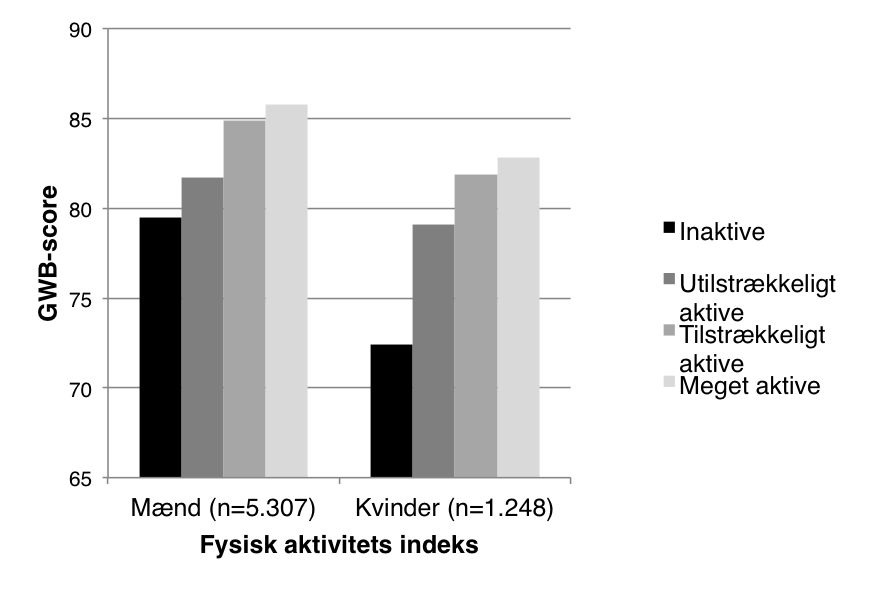
\includegraphics[width=0.6\textwidth]{figures/inaktivitet_gwb}
\caption{Fysisk inaktivitet sammenholdt med følelsesmæssig trivsel. På x-aksen fremgår grupperingen i fysisk aktivitetsniveau for hhv. mænd og kvinder. På y-aksen fremgår den gennemsnitlige GWB-score, hvilket indikerer følelsesmæssig trivsel på en skala fra $0-110$ \citep{galper2006}.}
\label{fig:inaktivitet_gwb}
\end{figure}

\begin{figure}[H]
\centering
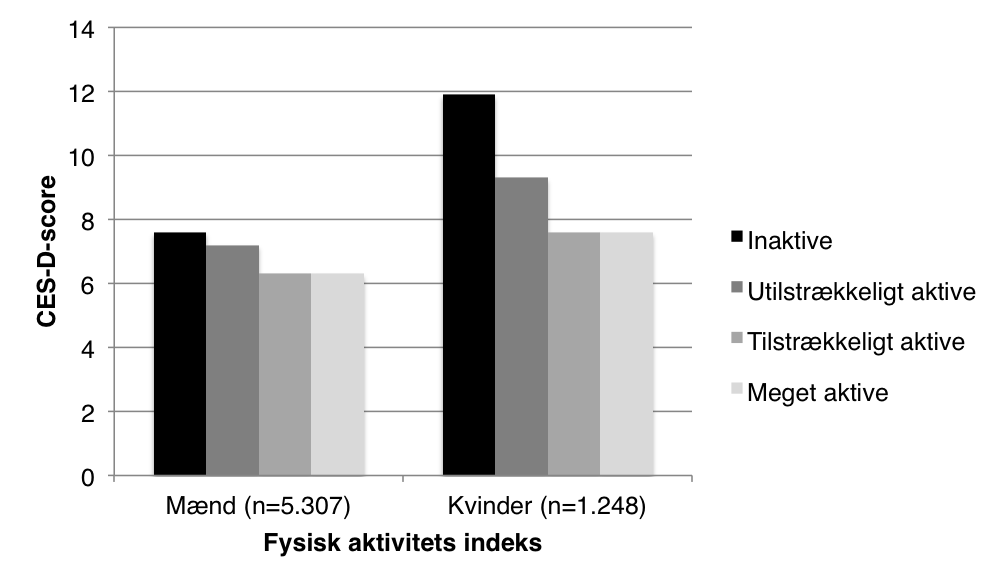
\includegraphics[width=0.6\textwidth]{figures/inaktivitet_dep}
\caption{Fysisk inaktivitet sammenholdt med depressionssymptomer. På x-aksen fremgår grupperingen i fysisk aktivitetsniveau for hhv. mænd og kvinder. På y-aksen fremgår den gennemsnitlige CES-D-score, hvilket indikerer depressive symptomer på en skala fra $0-60$ \citep{galper2006}.}
\label{fig:inaktivitet_dep}
\end{figure}

\noindent
Resultater herfra, som fremgår af \autoref{fig:inaktivitet_gwb} og \autoref{fig:inaktivitet_dep}, viser, at fysisk inaktive, især kvinder, har en højere tendens til depressive symptomer, end andre, der er mere fysisk aktive. På samme måde fremgik det af studiet, at fysisk inaktive forsøgspersoner  ikke trives følelsesmæssigt, som de, der er mere aktive \citep{galper2006}. 

Der er derved en sammenhæng mellem fysisk inaktivitet og psykiske følger, som eksempelvis depression og forværret følelsesmæssig trivsel \citep{galper2006}. Yderligere er der evidens for, at fysisk inaktivitet forværrer allerede eksisterende depressionstilstande samt dårlig følelsesmæssig trivsel \citep{motionsraad2007}.

% Afgrænsning af "sygdommen" til hypertension (en form for indledning til Birgithes afsnit)
\section{Sygdommen}
Det er påvist, at mange sygdomme har gavn af fysisk aktivitet som en behandling eller en metode til at forebygge sygdomsprogression. \citep{motionsraad2007,pedersen2011} Dette gælder forskellige typer sygdomme, og som påvirker forskellige aldersgrupper, hvorfor fysisk aktivitet generelt kan siges at være gavnligt, og hvorfor der eksisterer anbefalinger for alle omkring fysisk aktivitet. \citep{pedersen2011} Af denne grund vælges der til dette projekt at tage udgangspunkt i én sygdom og fysisk aktivitets påvirkning på netop denne sygdom.

Hypertension udgør en risikofaktor for følger som apopleksi, myokardieinfarkt, hjerteinsufcciens samt pludselig død, og ifølge nuværende definitioner af hypertension har omkring 20 \% af befolkningen denne sygdom. \citep{pedersen2011} Fysisk inaktivitet øger risikoen for hypertension, og motion har en synlig blodtrykssænkende effekt. \citep{olsen2015} Af denne grund vælges hypertension som udgangspunktet for dette projekt og denne problemanalyse. 
\section{Hypertension}

Af de 20 \% voksne danskere med hypertension, er omkring 30 \% ikke diagnosticeret. Dette skyldes, at der ofte ikke er tydelige symptomer på lidelsen \cite{kronborg2008}. Symptomer, der kan forekomme ved hypertension, er træthed, hovedpine, næseblod, hjertebanken og åndenød ved anstrengelse. Idet hypertension i de fleste tilfælde ikke medfører symptomer, opdages lidelsen derfor ofte ved et tilfælde \cite{olsen2015}.
% olsen2015: https://www.sundhed.dk/borger/patienthaandbogen/hjerte-og-blodkar/sygdomme/hoejt-blodtryk-hypertension/hypertension-symptomer/ 
% Ikke optimal kilde, men andre kilder siger det sammen, både danske og engelske. 
Der er en række sundhedsmæssige risici forbundet med hypertension, idet sygdommen medfører et øget pres på kroppens blodkar, hvilket forøger risikoen for udvikling af arteriesklerose, aneurismer, hjerteanfald og apopleksi. Længerevarende hypertension er af denne grund ofte årsag til kronisk nyresvigt og hjerte-kar-sygdomme \cite{martini2015}. Det kan være svært at estimere de nøjagtige tal for dødeligheden som følge af hypertension, idet patienterne ofte dør af følgevirkninger heraf, og årsagen til dødsfaldet kan være uklar. Ifølge Statens Institut for Folkesundhed er omkring 4 \% af alle dødsfald i Danmark relateret til hypertension \cite{juel2006}.
 
På trods af de sundhedsmæssige risici ved hypertension får 2/3 af de diagnosticerede patienter ikke tilstrækkelig behandling, således at de kan opnå det anbefalede blodtryk \cite{paulsen2012}.
Blodtryk er karakteriseret ved et systolisk og et diastolisk blodtryk, som henholdsvis er trykket i arterierne, når hjertet trækker sig sammen under systole, og trykket mellem to hjerteslag under diastole. Blodtryk skrives som ”systole/diastole” og måles i enheden millimeter kviksølv (mmHg). Det anbefales, at blodtrykket er under 140/90 mmHg, hvor et blodtryk over denne grænse betegnes hypertension. Er blodtrykket mellem 120/80 og 139/89 mmHg kaldes dette prehypertension, og der bør gøres opmærksom på dette for at undgå hypertension \cite{martini2015}.
% Martinibogen skal i kildelisten.

I de fleste tilfælde er årsagen til hypertension ukendt, men der er patientgrupper, der har særlig høj risiko for at udvikle hypertension. En lidelse, der ofte forbindes med hypertension, er diabetes. De to lidelser er begge resultatet af metabolisk syndrom, som er forstyrrelser i kroppens metabolisme og forekommer ofte grundet overvægt \cite{cheung2012}.

Behandling af hypertension kan ske farmakologisk eller non-farmakologisk. Ved farmakologisk behandling tages der højde for graden af hypertension, samt hvorvidt der er udviklet følgesygdomme. Alle patienter med hypertension bør behandles non-farmakologisk, hvilket betyder de får en række anbefalinger fra lægen, der bør følges. Herunder blandt andet ændring af motions- og kostvaner. Hypertensive patienter bør jævnligt ved konsultationer få kontrolleret blodtrykket, hvor lægen eller sygeplejersken desuden kan følge op på patientens vægt, kost og aktivitetsniveau. Normalt vil hypertension kunne behandles i almen praksis, men i tilfælde af behandlingsresistent hypertension, hvor blandt andet motion, kostændringer og formindsket alkoholindtag ikke kan udrede sygdommen, vil patienterne opleve at blive videresendt til en hypertensionsklinik \cite{lodberg2016, bech2015}.
\section{Nuværende metoder til aktivitetsmåling}

Inden for det danske sygehusvæsen, defineres fysisk aktivitet som værende en aktivitet, der forhøjer energiomsætningen. 
Dette betyder at alt mellem indkøb og gåture, til målrettet fysisk træning, kan defineres som værende fysisk aktivitet.\citep{gupta2013, terkelsen2015}

Sundhedsstyrelsen anbefaler desuden et aktivitetsniveau på mindst 30 minutters motion af moderat intensitet hver dag hele ugen. 
I forbindelse med dette, er moderat densitet blevet defineret som $40-59\%$ af maksimal iltoptagelse, $64-74\%$ af makspuls eller aktivitet, der gør patienten lettere forpustet, uden at forhindre muligheden for samtale. 
For at patienten bliver defineret som værende fysisk inaktiv, kræver det af den grund mindre end $2.5$ timers fysisk aktivitet om ugen.\citep{gupta2013}

I forbindelse med monitorering af aktivitetsniveauet for patienter ved klinikbesøg, kan den fysiske aktivitet bestemmes med udgangspunkt i flere forskellige undersøgelsesmetoder \citep{gupta2013}. 
Måden hvorpå aktiviteten monitoreres, kan opdeles i to kategorier: objektiv og subjektiv \citep{gupta2013, adamo2009}. 

%% Subejtiv metoder - Overordnet

En almindelig subjektiv metode, der anvendes er selvudfyldt dokumentation, der typisk giver et indblik i type af aktivitet, intensitet, hyppighed, samt tidsperiode for ydet aktivitet \citep{adamo2009}. Dertil er der forskellige måder at dokumentere den fysiske aktivitet, som f.eks. en aktivitetslog, aktivitetsdagbog, spørgeskemaer og lignende \citep{adamo2009}. 

%% Subjektive metoder - Konkrete beskrivelser

Spørgeskemaer tager udgangspunkt i faste spørgsmål omhandlende patientens fysiske aktivitet i løbet af dagligdagen \citep{muller2009}. 
Disse omhandler blandt andet transport til og fra arbejde, motionsvaner, tid brugt foran eksempelvis computer eller TV og ønsker om eventuelle ændringer af patientens aktivitetsvaner \citep{gupta2013, vestergaard2012}. 

Alternativt anvendes aktivitetsdagbøger \citep{muller2009} for at opnå en mere fyldestgørende indsigt i patientens aktivitetsmønster \citep{gupta2013}. 
Dagbogen fungerer som en logbog, hvori den primære aktivitet siden sidste notation, nedskrives med bestemte intervaller. 
Denne monitoreringsmetode giver et bedre indblik i patientens fysiske aktivitet gennem dagen, men er også mere tidskrævende at anvende for især patient men også læge.\citep{gupta2013}

%% Subjektive metoder - Overordnet ulemper 

Disse subjektive metode anvendes på grund af dens lave omkostning, lave patientbyrde, og generelle accept, samtidig med at den er velegnet til dokumentation af diversiteten i forhold til hvilken fysisk aktivitet der er ydet \citep{adamo2009}.

Denne type aktivitetsførelse forbindes dog med en fejlrepræsentation i forhold til den reelle fysiske aktivitet. Da det er en subjektiv dokumentationsmetoder, har patienter en tendens til enten at over- eller undervurderer deres egnen fysiske aktivitet \citep{adamo2009}. 
Et studie oplyser at 72 \% af patienter, af alderen 19 eller derunder, overestimerer deres fysiske aktivitet ved selvudfyldelse, i forhold til aktiviteten målt med objektiv/direkte aktivitetsførelse (accelerometer, pedometer, og lignende.) \citep{adamo2009}

Problematikken er således at de subjektive metoder ikke altid er i stand til at repræsentere den reelle fysiske aktivitet, selvom metoderne anses som værende valide \citep{pedersen2011, gupta2013}. 

%%%%%%%%%%%%%%%%%%%%%%%%%%%%%%%%%%%%%%%%%%%%%%%

Som et led i behandling af kronikere, såsom overvægtige eller diabetespatienter, udleveres der også skridttællere (accelerometre)\citep{muller2009, jensen2012, snorgaard2010}. 
Accelerometret vil give et mere detaljeret overblik over patientens aktivitetsmønster end spørgeskemaer og dagbøger, grundet muligheden for at monitorere kontinuert gennem længere tid. 
Der opstår dog komplikationer i forbindelse med anvendelsen, som følge af accelerometrets manglende evne til at opfange forskellige aktiviteter. 
Af den grund anvendes det kun til at danne et billede af, hvor meget tid patienten bruger på generel bevægelse. \citep{gupta2013}
\section{Alternative metoder til aktivitetsmåling}
Udover aktivitetsdagbog kan mere objektive målemetoder såsom pulsmåling, dobbeltmærket vand, accelerometer og skridttæller eller en kombination af flere anvendes til monitorering af aktivitetsniveauet hos individer [1?],\cite{motionsraad2007}. 

Pulsmåler bruges til at måle hjertefrekvensen. Der findes flere forskellige metoder til at detektere pulsen, her i blandt ved at måle den elektriske spændingsforskel som hjertet udsender ved hjælp af elektroder på hudens overflade, denne metode anvender typisk et bælte som brugeren har rundt om thorax \cite{motionsraad2007} [MANGLER]. En anden metode kaldet pulsoximeter, måler iltmætningen i blodet for heraf at kunne registrere pulsen [4?]. 

En pulsmåler indeholder elektroder, og ved kontakt med hudens overflade vil den elektriske spændingsforskel blive målt. 

Selvom pulsmålere giver et godt overblik over pulsfrekvensen ved et moderat eller højere intensitet, indebærer den også en begrænsning, ved registrering af pulsen i forbindelse med inaktivitet ved let aktivitet. For at pulsen ikke bliver påvirket af følelsesmæssige ændringer på kroppen, såsom forskrækkelse, hvor energiforbruget vil afvige lidt,  bruges flex-puls metoden. Denne metode har først en kalibreringsligning som bruges til at bestemme sammenhængen mellem arbejdsintensitet og puls hos den enkelte person. Ud fra kalibreringsligningen findes hvilepulsen, som kan bruges til at finde en flex-puls dvs. gennemsnittet mellem hvilepulsen og pulsen under letteste arbejde. \cite{motionsraad2007}

Dobbeltmærket vand er en metode som måler energiomsætning i kroppen. 

Skridttællerens primær funktion er at vise antal gået skridt indenfor en bestemt afstand. Skridttælleren kan hertil også måle antal forbrændte kalorier, totale træningstid og afstanden som brugeren har gået afhængigt af  designet. Skridttæller kaldes også pedometer, og findes i både mekanisk og elektronisk form. [1?]

Både skridttæller og aktivitetsarmbånd kan patienten monitorere på håndleddet og kan bruges under træning eller i hverdagen. Teknologierne kan bruges i forbindelse med selvkontrol af aktivitetsniveau, hvilket vil betyde at patienten har mere ansvar for monitorering af aktivitetsniveauet. 

Aktivitetsarmbånd, som også er et elektronisk måleinstrument, bruges af forskellige målgrupper for eksempel elite atleter/udøvere, som forbereder eller øver til en konkurrence. Aktivitetsarmbånd kan udover skridttælling også måle fysiske parametre som puls, søvn og kalorieindtag samt kalorier forbrændt. [2?] 

Aktivitetsarmbåndet kan blive synkroniseret til andre enheder såsom computer og mobil, på denne måde kan data også blive overført. 

%Et studie af Eduardo Ferriolli et al (Physical Activity Monitoring: A Responsive and Meaningful Patient-Centered Outcome for Surgery, Chemotherapy, or Radiotherapy?) målte 

%[1] http://www.explainthatstuff.com/how-pedometers-work.html 

%[2] 

%[3]http://sundhedsstyrelsen.dk/publ/MER/2007/FYSISK_INAKTIVITET-KONSEKVENSER_OG_SAMMENHAENGE2007.PDF (objektive målemetoder)

%[4] Pulse Oximetry Training Manual (se under mappen litteratur)

%Alt muligt andet pis:

%“Background: With the ever-increasing availability of health information technology (HIT) enabling health consumers to measure, store, and manage their health data (e.g., self-tracking devices) ”
%FYSISK_INAKTIVITET-KONSEKVENSER_OG_SAMMENHAENGE2007.PDF
\subsection{Teknologiafgrænsning}

Igennem en undersøgelse af hvilke funktioner, der vil være relevante i forbindelse med aktivitetstracking, opstilles krav som udgangspunkt for valget af den endelige teknologi. Kravene til funktion vil blive stillet ud fra den primære aktivitetsform hos patientgruppen, således aktivitetsarmbåndet er optimeret til netop denne aktivitetstype.

I Danmark stiger prævalensen af hypertension med alderen. Det ses blandt andet, at der kun er $1~\%$ af de $20-29$ årige, som lider af hypertension, mens omkring $69~\%$ af de $80-89$ årige har sygdommen \citep{olsen2015}. Som følge af den forøgede risiko for hypertension i sammenhæng med alderen, vil den primære anbefalede fysiske aktivitet for ældre over $65$ år, være $30$ minutters aktivitet med moderat intensitet om dagen og mindst $2$ gange $20$ minutters muskelstyrkende eller konditionsforøgende aktivitet om ugen \citep{pedersen2011}.

Hos ældre anses gang over $6$ km/t som konditionsforøgende aktivitet, og gang med $4-5$ km/t som moderat aktivitet. Med udgangspunkt i foregående, samt Sundhedsstyrelsens anbefalinger i 'Fysisk Aktivitet - Håndbog om forebyggelse og behandling' at tage udgangspunkt i gangregistrering med mulighed for udvidelse til svømning og cykling \citep{pedersen2011}.

\subsubsection{Krav til funktionalitet}

Såfremt aktivitetsarmbåndet skal anvendes i hverdagen, er det vigtigt, at det er kompakt og bærbar, samt at det ikke har behov for opladning på daglig basis. Som følge af at den primære aktivitet for patientgruppen er gang, er det vigtigt, at enheden kan måle dette præcist, således målingerne kan anvendes som valide data. 

Da Sundhedsstyrelsen også anbefaler svømning og cykling, hvis patienten har mulighed for dette, vil det være relevant, men ikke påkrævet, at aktivitetsarmbåndet har mulighed for at måle denne type aktivitet. Registrering af disse aktiviteter kræver både vandtæthed og GPS eller mulighed for kommunikation med en ekstern cykelcomputer på patientens cykel.

\subsubsection{Valg af aktivitetsarmbånd}

For at finde den mest optimale aktivitetsarmbånd til formålet, tages der udgangspunkt i studier, som har undersøgt præcisionen af forskellige aktivitetsarmbånd ved blandt andet antal skridt, energiforbrug og afstand. Ud over dette er brugerfladen også bedømt, hvorfor dette også er relevant at tage med i overvejelserne. Med udgangspunkt i de følgende studier, er det valgt at fokusere på Fitbit Flex, da dette indeholder den nødvendige teknologi til tracking, samt at muligheden for reproducering af målinger er høj \citep{kaewkannate2016}. Oven i dette udkom Fitbit Flex $2$ i $2016$, og den nye version giver mulighed for tracking af svømning, hvilket er væsentligt for patiengruppen \citep{fitbitflex}.

Både \citeauthor{evenson2015} og \citeauthor{kaewkannate2016} har undersøgt præcisionen af forskellige aktivitetsarmbånd. I 'Systematic review of the validity and reliability of consumer-wearable activity trackers' er der taget udgangspunkt i allerede eksisterende studier, for derved at opnå evidens for validitet og pålidelighed ved anvendelse af eksempelvis forskellige Fitbit og Jawbone modeller. Det andet studie, 'A comparison of wearable fitness devices', har undersøgt Fitbit Flex, Withing Pulse, Misfit Shine og Jawbone Up$24$. I studiet er både brugertilfredshed, repeterbarhed og præcision undersøgt, hvor aktivitetsarmbåndene testes ved normal gang, gang på trapper og gang på løbebånd. Samtidig testes muligheden for at gentage forsøget med samme resultat også, for at undersøge repeterbarheden \citep{evenson2015, kaewkannate2016}.

I studierne er det fundet, at Fitbit Flex's skridttæller har en høj præcision, som ifølge \citeauthor{kaewkannate2016} ligger mellem $96,4~\%$ til $99,6~\%$, afhængigt af om patienten bevæger sig på trapper, løbebånd eller fladt underlag. Her er præcisionen højest ved gang på fladt underlag, mens Fitbit uret scorer lavest ved gang på trapper eller løbebånd. Men som følge af de undersøgte aktivitetsarmbånd alle har en præcision omkring $95-99~\%$ afhængigt af gangtypen, argumentere dette for at valget af aktivitetsarmbånd ikke skal baseres på præcision, da denne er nær den samme for de undersøgte modeller \citep{kaewkannate2016}.

Fitbit Flex's målinger i forhold til antal skridt, afstand og energiforbrug varierer ikke markant fra hinanden ved samtidig brug af flere Fitbit Flex armbånd, hvorfor der ikke vil være stor ændring på målte data ved eventuel udskiftning af armbånd. Her er repeterbarheden for armbånd båret på højre og venstre håndled $0,90$ for skridt og $0,95$ for kilokalorier \citep{evenson2015}. For Fitbit Flex er repeterbarheden i det andet studie fundet mellem $0,72$ og $0,81$ afhængigt af gangtypen, mens den laveste og højeste repeterbarhed er $0,55$ og $0.89$ for det samlede studie. Her er repeterbarheden fundet ved at se på den samlede afstand forsøgspersonen er gået og den målte afstand for aktivitetsarmbåndene. \citep{kaewkannate2016}. Dette er blandt andet relevant ved dataindsamling til studier vedrørende effekten af armbåndet, da de optagede data dermed kan sammenlignes med større validitet. Samtidig undgåes problemer ved kalibrering, hvis patienten skal have byttet aktivitetsarmbåndet, som følge af fejlfunktion.

Yderligere fordele ved Fitbit Flex inkluderer muligheden for at gemme data i op til $30$ dage, muligheden for at sammenligne med andres aktivitet, vandtæthed og kompatibilitet med fitness-apps på smartphones og computer \citep{kaewkannate2016, fitbitflex}. Især de sociale egenskaber ved Fitbit's armbånd, samt muligheden for at tracke aktiviteten med apps, kan give anledning til øget aktivitetsniveau hos patienterne \citep{karapanos2016, rooksby2014}. Fitbit Flex er dog ikke udstyret med GPS, men hvis funktionen er nødvendig for tracking af bestemte aktiviteter, har patienten mulighed for at kombinere GPS-data fra eksempelvis smartphones med Fitbit's data. Som nævnt tidligere, har Fitbit Flex 2 mulighed for tracking af svømning, men som følge af mangel på studier vedrørende repeterbarheden og præcisionen af den nye model, fokuseres på den gamle model \citep{fitbitflex}.
\section{Problemformulering}

Her vil være en opsummering af problemanalysen, for at tydeliggøre hvorfor problemformuleringen lyder som følgende:

\textit{Hvilke effekter vil implementeringen af aktivitetsarmbånd til registrering og objektivisering af fysisk aktivitet hos hypertensive patienter have i den almene praksis?}

\textit{Hvilke påvirkninger vil implementeringen af aktivitetsarmbånd i den almene praksis til registrering og objektivisering af fysisk aktivitet have hos hypertensive patienter?}

%-------------METODE-----------------
\part{ Metode}
\chapter{Rapportens struktur} \label{metode}
Denne rapport tager udgangspunkt i metoden for en medicinsk teknologi vurdering (MTV), hvor en medicinsk problemstilling analyseres \citep{mtvhaandbog}. Yderligere er rapporten udarbejdet som et semesterprojekt på Aalborg Universitet, hvorfor den også tager udgangspunkt i problembaseret læring, hvor der opstilles et initierende problem, laves en problemanalyse og en problemformulering, der forsøges at besvare. 

\begin{figure}[H]
	\centering
	\includegraphics[width=0.5\textwidth]{figures/metodemodel}
	\caption{Model for den brugte metode i projektet.}
	\label{fig:metodemodel}
\end{figure}

\noindent
Som illustreret på \autoref{fig:metodemodel}, starter projektet bredt med et initierende problem, som analyseres og afgrænses i en problemformulering. Denne problemformulering forsøges besvaret gennem MTV-analyserne. 

MTV-analyserne belyser forskellige aspekter af teknologien ved at inddele MTV'en i fire områder: teknologi, patient, organisation og økonomi. %Der vælges at lægge mere vægt på udvalgte områder af MTV'en, da nogle af områderne er mere relevante for besvarelsen af problemformuleringen end andre.  

Hvert område vil have et tilhørende metodeafsnit til at beskrive, hvilke analysemetoder og fokuserende spørgsmål der bruges, og som er relevante for at kunne besvare den opstillede problemformulering. Den information som er nødvendig for at kunne besvare de fire MTV områder er i høj grad præget at eksisterende viden som er fundet ved at gennemføre en systematisk informationssøgning med udgangspunkt i de fire MTV områder. Metoden for informationssøgning beskrives yderligere i \autoref{sec:metode_soeg}. Ud over en systematisk informationssøgning indsamles information ud fra egne erfaringer om teknologien, hvilke kan være relevante for besvarelsen af visse MTV områder. Disse erfaringer ses især relevante på de områder hvor den eksisterende viden ikke har været tilstrækkelig for at kunne besvare de fokuserede spørgsmål under MTV analyserne.
%Måske en kilde til MTV bogen? :)

I syntesen vil de fire MTV-områder blive diskuteret, og der vil være en samlet konklusion på problemformuleringen ud fra delkonklusionerne i de fire MTV-analyser. 


En MTV er en vurdering baseret på forskning og kan herved anvendes som et evidensbaseret grundlag, når der skal tages beslutninger om, hvorvidt nye teknologier bør anvendes i sundhedsvæsenet. Målgruppen for en MTV er beslutningstagere, såsom politikere, ledelser på sygehuse og organisationer. De fire hovedområder indenfor MTV'en; teknologi, patient, organisation og økonomi, kræver forskellige metoder, videnskabelige teorier, forskingstilgange mm, og på baggrund af dette er der ofte forskellige fagfolk involveret i udarbejdelsen af en MTV \citep{mtvhaandbog}. 

Idet rapporten er udarbejdet af en sundhedsteknologi projektgruppe på 5. semester, og tager udgangspunkt i både metoden for en medicinsk teknolgodivurdering og problembaseret læring, har rapporten sandsynligvis ikke samme evidensniveau som en MTV udarbejdet af forskellige fagfolk. Dog anses det, at rapporten kan anvendes som udgangspunkt i en beslutningstagen eller til videreundersøgelser. 


\chapter{MTV-analyse}
Følgende kapitel beskriver de anvendte metoder i henholdsvis teknologi-, patient-, organisations- og økonomianalysen. Endvidere vil MTV-spørgsmålene til hver analyse fremgå. 

\section{Teknologi}\label{sec:metode_tek}
Teknologiafsnittet er opstillet ud fra en række MTV-spørgsmål, som vil beskrive teknologien og redegøre for og vurdere, hvilke teknologiske krav, Fitbit Flex skal opfylde for at kunne benyttes til at måle aktivitetsniveau hos hypertensive patienter. 
Foruden en tilpasset litteratursøgning ved brug af søgeprotokol, foretages beskrivelse af teknologien ud fra erfaringer ved anvendelse af software, der er relateret til teknologien.   
Herudover vil det blive undersøgt, hvilke effekter anvendelse af Fitbit Flex har på patientens sygdom.
 
\noindent
Dette giver anledning til følgende MTV-spørgsmål: 
\subsection{MTV-spørgsmål}
\begin{itemize}
\item Hvordan fungerer Fitbit Flex, og hvordan kan dette anvendes, således at en almen praktiserende læge får dokumenteret patientens aktivitetsniveau?
\item Repræsenterer Fitbit Flex den fysiske aktivitet tilstrækkeligt, til at data kan anvendes af praktiserende læger til vurdering af patientens fysiske aktivitetsniveau?
\end{itemize}

\section{Patient}\label{sec:metode_pat}
Til analyse af patienten og hvordan teknologien påvirker denne, anvendes \autoref{fig:patientaspekter}. Her analyseres sociale forhold, kommunikative forhold, økonomiske forhold, individuelle forhold og etiske forhold, samt sammenspillet mellem disse. I forhold til Fitbit Flex lægges der i denne analyse vægt på sociale forhold, herunder hvordan denne teknologi påvirker patientens arbejds- og uddannelsesliv, familie og livskvalitet, individuelle forhold, herunder hvordan patienten oplever teknologien, kommunikative forhold, samt etiske forhold, herunder risiko for misbrug af personlige data. 


\begin{figure}[H]
\centering
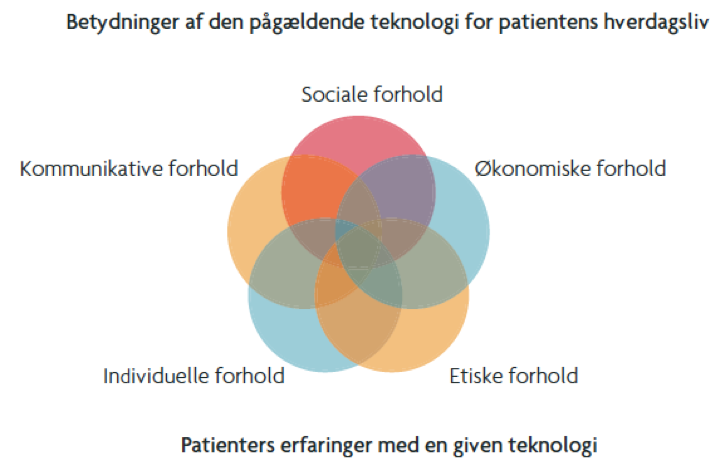
\includegraphics[width=0.8\textwidth]{figures/patientaspekter}
\caption{Patient-aspekter \citep{mtvhaandbog}.}
\label{fig:patientaspekter}
\end{figure}

\noindent
Dette giver anledning til følgende MTV-spørgsmål: 

\subsection{MTV-spørgsmål}
\begin{itemize}
\item Skal der være bestemte kriterier opfyldt for at patienten kan få udleveret en Fitbit Flex?
\item Er teknologien brugervenlig og motiverer den patienten til at få en mere aktiv hverdag?
\item Hvordan påvirker teknologien patienternes individuelle og sociale forhold i dagligdagen?
\item Hvor stor en andel af patienter oplever en positiv virkning ved anvendelse af teknologien, hvad er tidshorisonten for denne virkning, og hvad spiller en rolle for at teknologien giver et succesfuldt forløb?
\item Er der nogle etiske aspekter ved at monitorere patientens aktivitet, i så fald hvilke dilemmaer opstår heraf?
\end{itemize} 

\section{Organisation}\label{sec:metode_org}
Det ønskes at undersøge de organisatoriske forudsætninger samt mulige konsekvenser ved implementering af Fitbit Flex til monitorering af aktivitet i den primære sektor. Undersøgelsen tager udgangspunkt i den modificerede Leavitt organisationsmodel der ses af \autoref{fig:leavittmodel}, for at analysere konsekvenserne af en eventuel ændring i organisationen. Leavitts modificerede organisationsmodel benyttes, da denne tager højde for omgivelsernes påvirkning på teknologi, aktører, opgaver, struktur, disses indbyrdes påvirkning og påvirkning på omgivelserne. 
Teknologi omhandler arbejdsprocesser, procedurer og rutiner, i relation til teknologien.  
Aktører er de ansatte i organisationen, og deres holdninger og ekspertise i relation til organisationens opgaveløsninger. 
Opgaver dækker over de opgavetyper som organisationen forsøger at løse. 
Struktur omhandler formelle mønstre i organisationen, som arbejdsdeling og formalisering.  
Omgivelser er udvalgte interessenter, der er relevante i forhold til de organisatoriske ændringer. 

\begin{figure}[H]
\centering
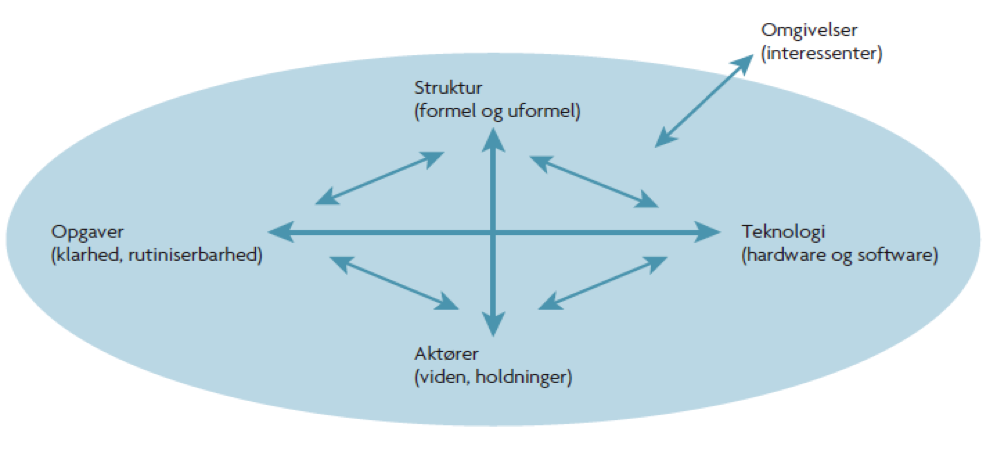
\includegraphics[width=0.9\textwidth]{figures/leavitt}
\caption{Leavitts modificerede organisationsmodel. Pilen mellem de forskellige områder betegner sammenspillet mellem dem. Dertil står omgivelser uden for de andre fire områder, da dette betgener hvem der har interesse for de organisatoriske ændringer der vil forekomme \citep{mtvhaandbog}.}
\label{fig:leavittmodel}
\end{figure}
\noindent
Dette giver anledning til følgende MTV-spørgsmål:

\subsection{MTV-spørgsmål}
\begin{itemize}
\item Hvordan passer Fitbit Flex i den primære sundhedssektor? 
\item Hvilke krav vil implementeringen stille til alment praktiserende læger, og hvem skal stå for en eventuel efteruddannelse? 
\item  Hvordan vil patientfordelingen mellem den primære og sekundære sundhedssektor blive påvirket, og hvad vil en ændring i arbejdsfordelingen medføre?
\end{itemize}

\section{Økonomi}\label{sec:metode_oeko}
I økonomianalysen undersøges mulige omkostninger, der kan forekomme ved implementering og anvendelse af Fitbit Flex som monitoreringsenhed for aktivitet til brug i almen praksis.
Ligeledes undersøges omkostninger for den nuværende monitoreringsmetode, samt hvilke økonomiske konsekvenser, der forekommer, når patienten ikke dyrker den anbefalede mængde motion.
Det ønskes at lave cost-effectiveness og cost-utility analyser for at afgøre, om Fitbit Flex skal implementeres. I cost-effectiveness analysen opgøres omkostninger og konsekvenser ved den nuværende monitoreringsmetode og Fitbit Flex for at afgøre, hvilken teknologi der er mest omkostningseffektiv i forhold til både valuta og antal vundne leveår. Cost-utility analysen benyttes til at tage højde for kvalitetsjusterede leveår (QALY), hvor de vundne leveår kvalitetsjusteres med den helbredsrelaterede livskvalitet \citep{mtvhaandbog}.
I denne analyse vil blive fremhævet mulige sundhedsmæssige resultater som følge af implementeringen af Fitbit Flex, i forhold til udgifterne dertil, uden at lave en egentlige cost-effectiveness eller cost-utility analyser, eftersom de benyttede værdier i analysen er estimerede.  
Disse estimerede værdier er baseret på udregninger ud fra funden litteratur omkring sundhedsøkonomi.

\noindent
Dette giver anledning til følgende MTV-spørgsmål: 

\subsection{MTV-spørgsmål}
 
\begin{itemize}
\item Hvad er omkostningerne ved nuværende monitoreringsmetode, samt konsekvenserne ved utilstrækkelig aktivitetsydelse? 
\item Hvilke omkostninger er forbundet med brug af Fitbit Flex til patienter med hypertension, og hvad er den økonomiske konsekvens af dette, hvis brug af aktivitetsarmbånd resulterer i et øget antal kvalitetsjusterede leveår?
\end{itemize}


%  Søgeprotokollen findes i \autoref{app:soegeprotokol}.

%-------------MTV--------------------
\part{ MTV-analyse}
%-------------Teknoglogi-------------
Teknologi
Dette kapitel har fokus på det teknologiske element, hvor teknologien vil blive karakteriseret, analyseret og vurderet. Dette gøres i henhold til metodeafsnittet (???). Der er opstillet en række MTV spørgsmål, som vil redegøre for og vurdere, om aktivitetsarmbånd fra et teknologisk synspunkt kan anvendes til at måle aktivitetsniveau hos patienter med ’sygdom’. Herudover vil det blive undersøgt, hvilke følgevirkninger anvendelse af aktivitetsarmbånd har på patientens sygdom. (Eller noget??)

Hvordan måles patienters aktivitet på nuværende tidspunkt? (I problemanalysen?)

Hvordan fungerer en aktivitets tracker/armbånd(??), og hvordan kan denne anvendes i medicinsk sammenhæng, således at en almen praktiserende læge får dokumenteret patientens aktivitetsniveau?
(Er der på nuværende tidspunkt læger, der anvender aktivitetsarmbånd, hvordan får de data fra aktivitetsarmbåndet?)

Hvor stor nøjagtighed/pålidelighed er det nødvendigt, at aktivitets armbånd har, hvis de skal anvendes til det ønskede formål, og hvor nøjagtige/pålidelige er de eksisterende aktivitetsarmbånd? (eller omvendt – Hvor nøjagtige er aktivitetsarmbånd, og er pålideligheden stor nok til at kunne anvendes i sundhedssektoren?)

Hvilken effekt (eller konsekvenser, følgevirkninger?) har anvendelsen af aktivitetsarmbånd til dokumentering af aktivitetsniveau på patientens sygdom?

(Hvilke problematikker kan opstå ved brug af aktivitetsarmbånd?) fneh….
% Indhold i afsnittet\\
%\section{Besvarelse}
Indhold: Dette afsnit vil indeholde forskellige underemner, der vil beskæftige sig med forskellige aspekter, så MTV-spørgsmålene kan besvares. 
\section{Teknologibeskrivelse} \label{sec:teknologibeskrivelse}
Aktivitetsarmbånd bliver i stigende grad mere udbredt. Ifølge International Data Corporation er der sket en stigning i salget af aktivitetsarmbånd fra $11,8$ millioner enheder i første kvartal af 2015 til $19,7$ millioner i første kvartal af 2016 \citep{IDC2016}.

Det er fundet, at Fitbit udgør en stor andel af markedet for aktivitetsarmbånd og, at der fra første kvartal i 2015 til første kvartal i 2016, er sket en stigning i salget på $1$ million enheder \citep{IDC2016}.  
Fitbit Flex ses på \autoref{fig:fitbitflexarmbånd}. 

\begin{figure}[H]
	\centering
	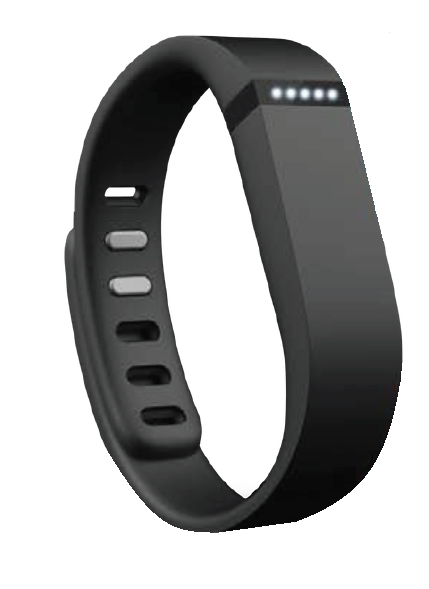
\includegraphics[width=0.3\textwidth]{figures/fitbitflex}
	\caption{Fitbit Flex armbånd \citep{fitbitflex}.}
	\label{fig:fitbitflexarmbånd}
\end{figure}

\noindent
Overordnet består Fitbit Flex med tilbehør af en flex tracker, oplader kabel, trådløs synkroniserings dongle og armbånd til flex tracker \citep{fitbitflex}. Disse kan ses af \autoref{fig:fitbitflexindhold}. 

\begin{figure}[H]
	\centering
	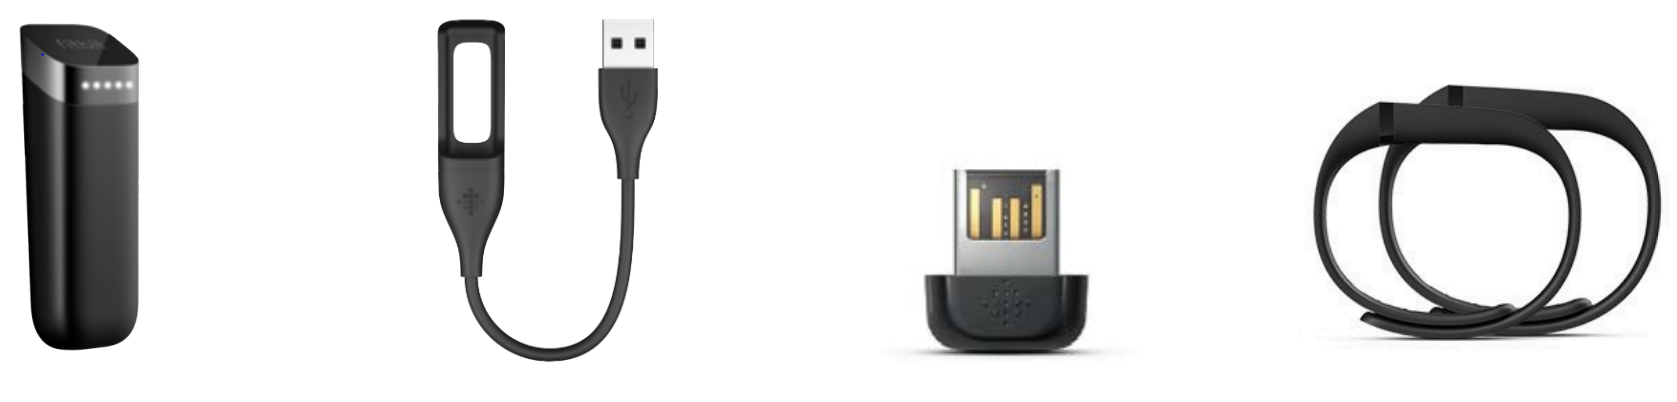
\includegraphics[width=0.6\textwidth]{figures/fitbitflexindhold}
	\caption{Fra venstre mod højre ses de forskellige dele af Fitbit Flex pakken, bestående af flex tracker, oplader kabel, trådløs synkroniserings dongle og armbånd \citep{fitbitflex}.}
	\label{fig:fitbitflexindhold}
\end{figure}

\noindent
Fitbit Flex er i stand til at måle antal minutter, brugeren er aktiv, længden samt kvalitet af søvn og antal skridt, hvorudfra den kan estimere forbrændte kalorier og tilbagelagt afstand. 
For at brugeren kan se den registrerede aktivitet, som er blevet opsamlet af armbåndet, skal dette synkroniseres med en kompatibel enhed, da armbåndet kun besidder et display bestående af fem LED'er \citep{fitbitflex}. 

Synkronisering foregår trådløst ved brug af bluetooth low energy (BLE) og kan foregå mellem forskellige enheder såsom smartphone og computer. 
Synkronisering mellem flex tracker og computer kræver dog anvendelse af den trådløse synkroniserings dongle, der ses af \autoref{fig:fitbitflexindhold}.
Forudsætninger for, at data kan synkroniseres er, at en kompatibel enhed har den korrekte applikation installeret, hvor synkroniseringen ellers sker automatisk idet applikationen åbnes.  
Yderligere skal der oprettes en brugerkonto på \url{www.fitbit.com}, hvor brugeren oplyser personlige informationer: køn, alder, højde og vægt. Dette er nødvendigt i forhold til optimering af dataopsamling og estimering af forbrændte kalorier \citep{fitbitflex}.  

Gennem applikationen visualiseres den registrerede aktivitet, hvor brugeren har mulighed for at se data fra anvendelsesperioden. Data kan også observeres på Fitbits hjemmeside, hvor det er muligt at logge ind via brugerkontoen. 
Således ville alle i besiddelse af en given brugerkonto have adgang til den synkroniserede data, uden fysisk at have hverken bruger eller armbånd til stede. 
Til den daglige aktivitet har brugeren mulighed for at sætte bestemte mål til den fysiske aktivitet. Alt efter hvilke mål brugeren sætter for sig selv, kan progressionen ses ud fra de fem LED'er på armbåndet ved, at brugeren trykker to gange på armbåndet \citep{fitbitflex}.   

Når ét af brugerens mål gennemføres, visualiseres dette ved, at de 5 LED'er blinker, og at armbåndet vibrerer. 
Fitbit Flex er ikke i stand til at visualisere batteriniveauet for armbåndet, dette kan dog ses ved brug af applikationen. 
Hukommelsen i flex trackeren tillader detaljeret data at blive lagret i perioder op til 7 dage og består af minut til minut målinger.  
Yderligere lagres summeringer af daglig aktivitet i op til 30 dage. 
Ved jævnlig synkronisering er det muligt for brugeren at bevare detaljeret data, da informationen tilknyttes brugerkontoen. 
Fitbit anbefaler én daglig synkronisering, dog er det ikke en nødvendighed \citep{fitbitflex}. 

\subsection{Hardware}
Fitbit Flex trackeren har forskellige hardware elementer, hvorfra trackeren signalerer og detekterer fysisk aktivitet. Hardwaren i trackeren udgøres af et display, batteri, en sensor og en motor \citep{fitbitflex}.
 
\subsubsection{Display} 
Flex trackeren er udstyret med fem LED'er, der ved forskellige operationstilstande, såsom alarm, aktivitet eller søvntracking, signalerer til brugeren. 
LED'erne kan fungere som indikator for progressionen i forhold til det brugerdefinerede fysiske mål for dagen. Hertil vil hver LED repræsentere en procentvis progression i intervaller af $20~\%$. Ved $73~\%$ progression af det fysisk mål, vil de første tre LED'er lyse, og den fjerde vil blinke. Dette indikerer, at brugeren har nået $60~\%$ af målet, og at brugeren nu befinder sig mellem $60~\%$ og $80~\%$. 
Det samme gør sig gældende, når flex trackeren sættes til opladning. Her indikerer LED'erne, hvor langt armbåndet er fra fuld opladning, som signaleres ved, at alle fem LED'er lyser \citep{fitbitflex}. 
%I tilfælde af synkroniseringsfejl vil dette også fremgå af LED'erne. Her vil armbåndet lyse med et mønster, skiftevis mellem at have ingen eller alle LED'er tændt. 
%Ved manuel aktivering og de-aktivering af sleep mode, vil LED'erne indikere dette gennem forskellige indikationsmønstre.

\subsubsection{Sensor} 
Flex trackeren registrerer den fysiske aktivitet ved anvendelse af et 3-akses mikro elektro-mekanisk accelerometer, hvilket er den eneste sensor, som er implementeret i armbåndet. Et 3-akses accelerometer kan måle i x-, y- og z-retning og kan give et udtryk for ændringerne i hastigheden \citep{ravi2005}. Ud fra algoritmer analyseres bevægelsesmønstre, hvorved der kan oplyses hvor mange skridt, der er foretaget under løb eller gang, samt den tilbagelagte afstand. 

\subsubsection{Motor}
Flex trackeren er udstyret med en vibrationsmotor, der aktiveres under forskellige funktioner, når armbåndet anvendes. Disse fungerer i sammenspil med displayet som et kommunikationsredskab for brugeren. Vibration aktiveres ved anvendelse af alarmfunktion, og ved aktivering eller deaktivering af sleep mode, samt når det daglige fysiske mål nås. 

\subsubsection{Batteri} 
Fitbit Flex indeholder et genopladeligt batteri, der oplades ved brug af det medfølgende kabel. Dette ses af \autoref{fig:fitbitflexindhold}. Kablet tilsluttes en computer og opladningen begynder, hvis computeren er tændt. 
Levetiden på batteriet er op til 5 dage afhængigt af, hvor ofte armbåndet synkroniseres for at visualisere progressionen.


\subsection{Software}
Applikationen, som kan installeres på smartphone, er brugerfladen hvorfra den synkroniserede data formidles til brugeren. Beskrivelsen af brugerfladen er gjort med udgangspunkt i applikationen og hjemmesiden, som følge af Fitbit ikke har en konkret guide til den samlede software. I brugerfladen oplyses skridt, forbrændte kalorier med mere. 
Alt efter brugerens interesser, kan der også udfyldes informationer omkring indtaget kost ved brug af applikationen. Brugeren kan ud fra dette få et estimat af, hvor mange kalorier, der indtages, hvortil dette kan sammenlignes med antal kalorier forbrændt. Anvendelsen af denne funktion er dog ikke en nødvendighed for anvendelsen af Fitbit Flex eller applikationen, dog kunne dette give en praktiserende læge indblik i, om patienten overholder anbefalingerne for hypertensive patienter, både i forhold til kostvaner og fysisk aktivitet.

\begin{figure}[H]
	\centering
	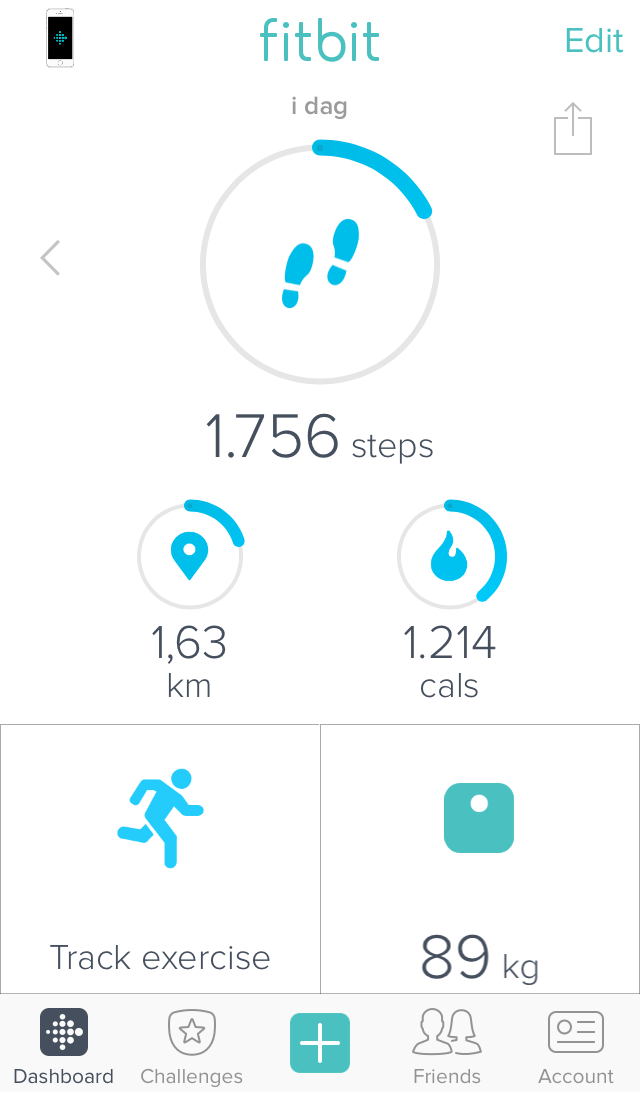
\includegraphics[width=0.45\textwidth]{figures/burgerfladeoversigt}
	\caption{Oversigt over fysisk aktivitet, der vises idet applikationen åbnes. Her ses blandt andet antal skridt taget, tilbagelagt afstand og kalorier forbrændt.}
	\label{fig:brugerfladeoversigt}
\end{figure}

\noindent
Af \autoref{fig:brugerfladeoversigt} ses oversigt over den registrerede aktivitet, som er målt gennem armbåndet. Her ses antal skridt taget, tilbagelagt afstand og kalorier forbrændt. Af oversigten ses også, hvor langt brugeren er fra at opfylde de forskellige aktivitetsmål og er repræsenteret af den blå cirkel omkring de forskellige angivelser. 
I bunden ses fire forskellige oversigter, hvor der fra venstre mod højre ses 'Dashboard', 'Challenges', 'Friends' og 'Account'. Plus-tegnet i midten fungerer som en genvej til forskellige funktioner under de fire oversigter. 
'Dashboard' er den overordnede oversigt, som oplyser det førnævnte.
'Challenges' viser en oversigt over tilvalgte aktivitetsudfordringer, hvor brugeren har mulighed for at opstille udfordringer med venner samt andre brugere af applikationen. 
'Friends' giver brugeren et overblik over venner, der er tilføjet til applikationen. 
'Account' viser et overblik over, hvilken bruger, der er logget ind, og hvilken Fitbit enhed, der er tilsluttet applikationen. Yderligere kan der foretages ændringer af profil og mål for daglig fysisk aktivitet. 

En detaljeret oversigt over ydet aktivitet kan ses under den overordnede oversigt ved at trykke på de specifikke målinger. Ved at trykke på 'Steps' ses eksemplet, der fremgår af \autoref{fig:brugerfladesteps}.  

 % Kan ikke henvise til disse figurer.
\begin{figure}[H]
	\centering
	\begin{minipage}{0.48\textwidth}
		\centering
		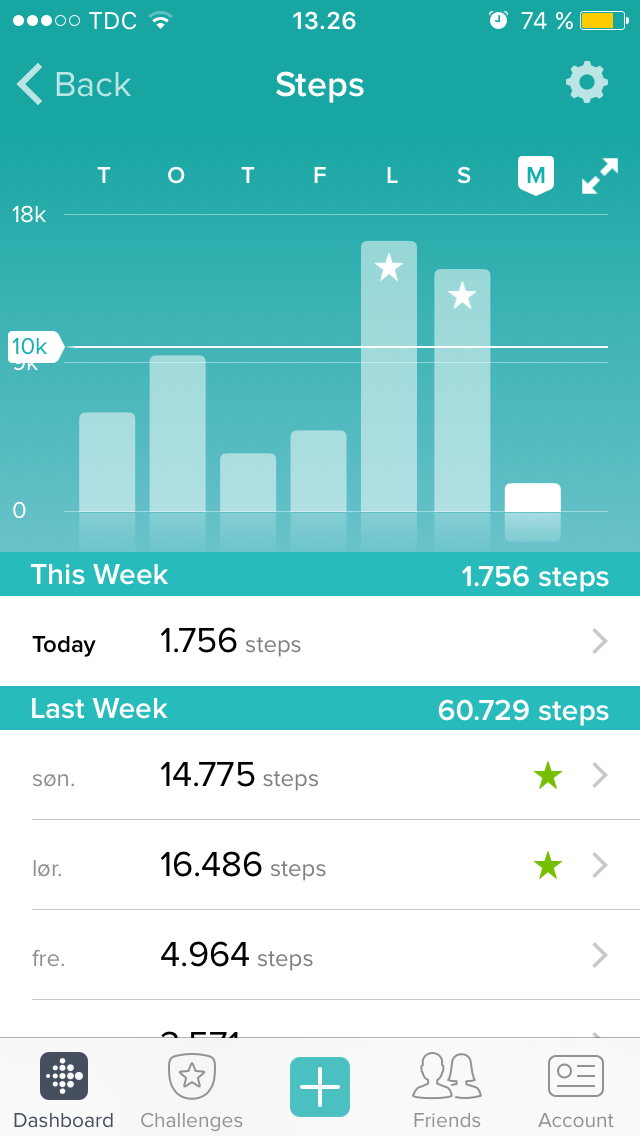
\includegraphics[width=0.8\linewidth]{figures/brugerfladesteps}
		\caption{Oversigt over skridt taget for den  forudgående uge delt op i ugens dage, som graf (øverst) og tabel (nederst).}
		\label{fig:brugerfladesteps}
	\end{minipage}%
	\hspace{3mm}
	\begin{minipage}{0.48\textwidth}
		\centering		
		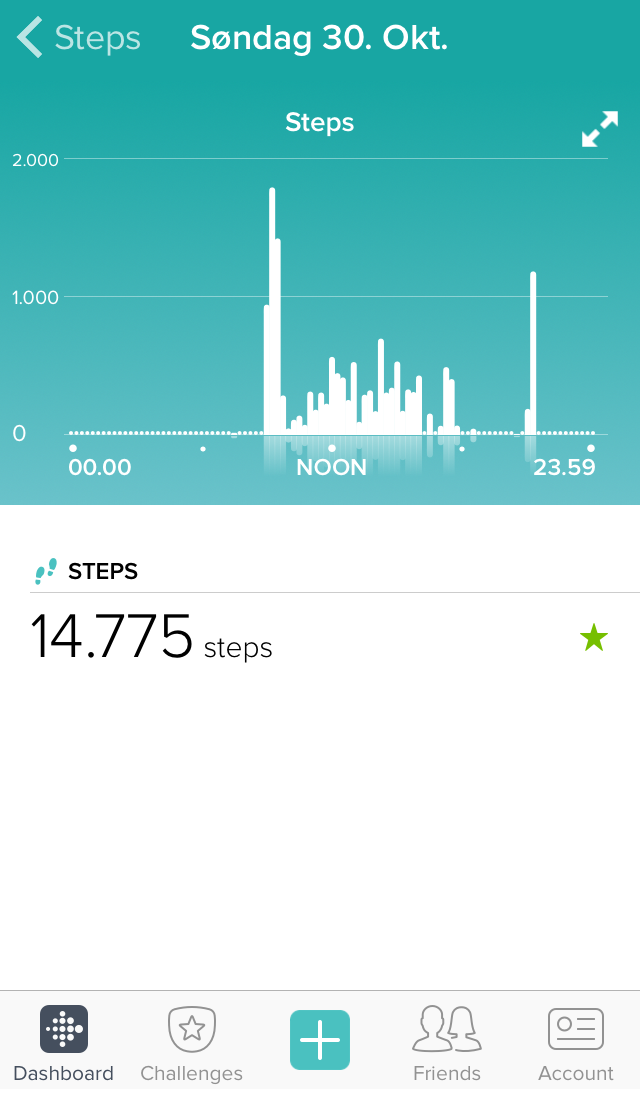
\includegraphics[width=0.8\linewidth]{figures/specifiksteps}
		\caption{Oversigt over skridt taget for én dag, som graf fordelt på døgnets timer (øverst) og i endeligt antal skridt (nederst).}
		 \label{fig:specifiksteps}
	\end{minipage}
\end{figure}

\noindent
Af \autoref{fig:brugerfladesteps} ses der øverst en graf over antal skridt taget inden for den sidste uge. Af grafen ses en hvid tværgående linje, der repræsenterer målet for antal skridt for dagen. Hertil ses at dage, hvor målet er blevet opfyldt, markeres med en stjerne.

Under grafen ses en oversigt over antal skridt taget for de forhenværende dage, rækkende tilbage til den første anvendelsesdato. Heraf ses ligeledes at dagene, hvor målet nåes, er indikeret med en stjerne. 

Ved at trykke på den givne dag eller en af de forhenværende dage, kan der ses en mere detaljeret oversigt over antal skridt taget i løbet af den pågældende dag. Dette ses af \autoref{fig:specifiksteps}, hvor det er muligt at se på hvilke tider af dagen, brugeren er mest aktiv.  

\subsubsection{Brugerflade på nettet}

Det sociale aspekt af Fitbit's brugerflade giver mulighed for at følge andre brugere, hvorved det er muligt at følge deres aktivitet gennem Fitbit's hjemmeside. Afhængigt af privatindstillinger, kan antal skridt, tilbagelagt afstand, søvnkvalitet, vægt og tid med forskellige aktivitetsniveauer ses på brugerens profil. Her er det muligt at se de førnævnte detaljer om brugeren for de seneste $30$ dage, som vist på \autoref{fig:netbruger}.

\begin{figure}[H]
	\centering
	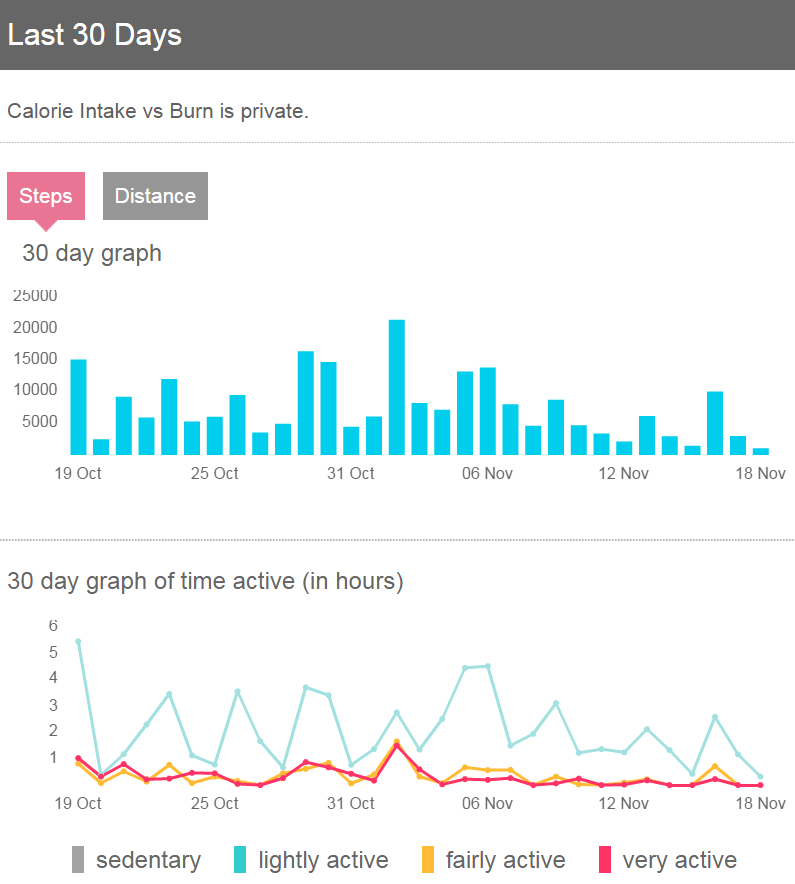
\includegraphics[width=0.45\textwidth]{figures/Netbruger}
	\caption{Oversigt over fysisk aktivitet hos en bruger, som set på Fitbit's hjemmeside}
	\label{fig:netbruger}
\end{figure}

Ved at holde markøren over forskellige områder af graferne og søjlerne på \autoref{fig:netbruger}, er det muligt at se præcise tal for aktiviteten. Søjlerne vist øverst på figuren, er antallet af skridt brugeren har taget, og kan med knappen "Distance" ændres, således den tilbagelagte afstand vises i stedet. Graferne nederst på figuren viser antal timer med let, middel og intens aktivitet, hvorved det er muligt at se hvor mange aktive timer, brugeren har i løbet af dagen. 

\subsection{Brugertilpasning} \label{sec:brugertilpasning}
Der er forskellige muligheder for at tilpasse armbåndet optimalt til den givne bruger. Heriblandt er der mulighed for at udskifte armbåndet til andre længder, og at tilpasse skridtlængden til den enkelte bruger. Foruden dette tilegner armbåndet sig til at blive brugt under forskellige vejrforhold, da Fitbit Flex er vandafvisende. 

\subsubsection{Forskellige Fitbit Flex armbånd}
Brugeren har mulighed for at vælge armbånd i to forskellige længder. Dette tillader muligheden for bedre tilpasning omkring håndleddet. Armbåndene kan ligeledes fås i forskellige farver.

\subsubsection{Kalibrering af skridtlængde}
Applikationen vurderer som standard brugerens skridtlængde ud fra de angivne oplysninger ved oprettelsen af brugerkontoen. Brugeren har dog mulighed for at kalibrere denne værdi i tilfælde af, at brugeren opdager uoverensstemmelse mellem registrerede værdier og reelle værdier. Brugeren kan under indstillinger i applikationen ændre den pre-definerede skridtlængde til en mere passende værdi. Fitbit oplyser på deres support-hjemmeside guidelines for, hvordan brugeren selv udregner værdier til en mere passende skridtlængde.   

\begin{comment}
Hvad består teknologien af?
Hvor udbredt er teknologien?
Hvordan tilpasses teknologien den enkelte person?
Levetid for teknologien?
Hvilke muligheder er der for lagring og videregivelse af information til en læge?
\end{comment}

\subsection{Fordele og begrænsninger ved teknologien}
Sammenlignes anvendelse af aktivitetsarmbåndet Fitbit Flex med nuværende anvendte metoder til objektivisering af aktivitetsniveau i almen praksis, er der forskellige fordele og begrænsninger ved denne alternative metode. Som tidligere nævnt giver anvendelsen af aktivitetsarmbånd den almen praktiserende læge en mere nøjagtig vurdering af en patients aktivitetsniveau sammenlignet med subjektive besvarelser såsom spørgeskemaer.

Informationer om aktivitetsniveauet opsamles automatisk, og det er dermed ikke nødvendigt for patienten selv at holde styr på, hvor meget aktivitet, der udføres. Lægens opfattelse af, hvor meget fysisk aktivitet patienten udfører afhænger derved heller ikke af patientens hukommelse eller evne til at formidle. Det giver lægen en mere præcis oversigt over aktiviteten udført over tid, og dette kan hjælpe med at se en eventuel udvikling eller tilbagegang i aktivitetsniveauet hos patienten. 

Det er desuden ikke nødvendigvis ekstra tidskrævende at anvende aktivitetsarmbåndet, hvis patienten har modtaget tilstrækkelig information om, hvordan udstyret anvendes korrekt. Problemer kan opstå, hvis patienten oplever besvær ved anvendelsen af aktivitetsarmbåndet, og ikke bruger det korrekt eller vælger helt at undgå at bruge det.

Fitbit Flex har som tidligere nævnt ikke mulighed for at registrere svømning. Udfører en patient fysisk aktivitet i form af svømning, kan dette ikke måles med aktivitetsarmbåndet. Dette kan medføre at lægen får en forkert objektivisering af patientens aktivitetsniveau, hvis patienten ikke har meddelt lægen, at patienten foruden den registrerede aktivitet også svømmer. Sammenlignet med de subjektive metoder, der anvendes i klinikkerne, kan alle former for fysisk aktivitet medtages på én gang ved besvarelse af eksempelvis spørgeskema eller under samtale om patientens aktivitetsniveau.
En ulempe ved anvendelse af Fitbit Flex sammenlignet med andre aktivitetsarmbånd er, at der ikke er indbygget GPS i denne. Ønsker patienten at vide placering, skal en ekstern GPS, eksempelvis på en smartphone, anvendes. Det er dog ikke en nødvendighed for lægen at vide placeringen, da lægen som udgangspunkt kun er interesseret i at kende aktivitetsniveauet. Cykler patienten, kan GPS være en metode til at holde styr på afstanden, der er tilbagelagt. Samme problemstilling som ved svømning kan her opstå, hvis aktivitetsarmbåndet ikke registrerer aktiviteten under cykling.
 
En begrænsning i forhold til aktivitetsarmbånd sammenlignet med nuværende metoder er, at det er en mere teknologisk metode, der kan kræve adgang til smartphone eller PC og muligvis internet. Størstedelen af de hypertensive patienter er en del af den ældre befolkningsgruppe. I 2014 var der ifølge Danmarks Statistik 41 \% af de 75-89 årige, der aldrig har brugt internettet \citep{dst2014}. Hvis lægen skal have mulighed får at tilgå patientens data vedrørende aktivitetsniveauet uden, at patienten er fysisk til stede, eksempelvis ved telefonkonsultationer, er det nødvendigt, at patienten har adgang til internettet for at synkronisere data fra aktivitetsarmbåndet med dennes brugerkonto.

Som nævnt i \autoref{sec:teknologibeskrivelse} skal Fitbit Flex synkroniseres med en smartphone eller PC for at kunne se den registrerede aktivitet. Dette kræver, at patienten er i besiddelse af en af disse, hvis patienten selv ønsker at følge med i aktiviteten. Har patienten ikke mulighed for at komme i besiddelse af smartphone eller PC, kan detaljeret data lagres i aktivitetsarmbåndet i op til syv dage. Dette kan dog imødegås ved, at lægen tjekker data fra aktivitetsarmbåndet indenfor de syv dage, hvis det ønskes at se detaljeret data. Ellers kan Fitbit Flex gemme mindre detaljeret data i op til 30 dage. Fitbit Flex har desuden et batteri, der genoplades ved at koble den til en PC. 

\subsection{Nøjagtighed af aktivitetsmåling}
Indhold: Dette afsnit skal indeholde analyse af, hvor nøjagtig/pålidelig teknologien er ved repræsentation af fysisk aktivitet. Herunder vil vi gerne komme ind på, hvad nøjagtigheden af teknologien betyder for brugeren og brugen af teknologien; hvad det betyder, hvis den underestimerer mængden af aktivitet, og er teknologien nøjagtig/pålidelig nok til brug i almen praksis?

\section{Delkonklusion}
Indhold: Dette afsnit vil indeholde en delkonklusion af denne del af MTV'en og dette kapitel, som forhåbentligt vil lede frem til en endelig konklusion i syntesen. 

%-------------Patient----------------
\chapter{Patienten}
Dette kapitel har fokus på patientaspektet, hvor teknologiens påvirkning på patienten vil blive karakteriseret, analyseret og vurderet. 
\section{Metode}
Til analyse af patienten og hvordan teknologien påvirker denne, anvendes \autoref{fig:patientaspekter}. Her analyseres sociale forhold, kommunikative forhold, økonomiske forhold, individuelle forhold og etiske forhold, samt sammenspillet mellem disse. I forhold til Fitbit Flex lægges der i denne analyse vægt på sociale forhold, herunder hvordan denne teknologi påvirker patientens arbejds- og uddannelsesliv, familie og livskvalitet, individuelle forhold, herunder hvordan patienten oplever teknologien, kommunikative forhold, samt etiske forhold, herunder risiko for misbrug af personlige data. 
%(Nogle af aspekterne kan vægte mere end andre alt efter hvilken teknologi der er tale om, med en aktivitets tracker er det nok mest, (listet i prioriteret rækkefælge) sociale forhold, herunder hvordan det påvirker patientens arbejds/uddannelses liv, familie, fritid og generel livskvalitet. Individuelle forhold, herunder hvordan patienten oplever teknologien, tilfredshed, motivation, tryghed mm. Kommunikative forhold, herunder hvordan der kommunikeres fra f.eks. sygehus til patient og omvendt, fra teknologi til patient og sygehus. Etiske forhold kan måske indgå i og med at patienternes aktivitet måles og bliver opsamlet som data, disse data bliver set af patienten og lægen, måske deler patienten sine resultater over sociale medier, kan disse data misbruges af andre? GPS, placering kan ses. Økonomiske forhold, altså om teknologien giver udgifter for patienten eller påvirker vedkommendes økonomi.).


\begin{figure}[H]
\centering
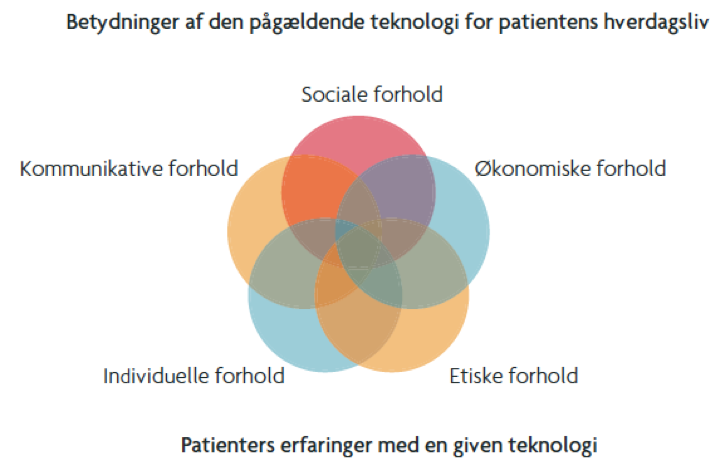
\includegraphics[width=0.8\textwidth]{figures/patientaspekter}
\caption{Patient-aspekter \citep{mtvhaandbog}.}
\label{fig:patientaspekter}
\end{figure}

\noindent
Dette giver anledning til følgende MTV-spørgsmål: 
%(Inklusions og eksklusions kriterier skal muligvis opstilles for at kunne fokusere modellen på den målgruppe som vi vælger at fokusere på)


\subsection{MTV-spørgsmål}
\begin{itemize}
\item Skal der være bestemte kriterier opfyldt for at patienten kan få en aktivitets tracker?
\item Er teknologien brugervenlig og motiverer den patienten til at få en mere aktiv hverdag?
\item Hvordan påvirker teknologien patienternes individuelle og sociale forhold i dagligdagen?
\item Hvor stor en andel af patienter oplever en positiv virkning ved anvendelse af teknologien, hvad er tidshorisonten for denne virkning, og hvad spiller en rolle for at teknologien giver et succesfuldt forløb?
\item Hvor meget ansvar har patienten ved anvendelsen af teknologien?
\item Er der nogle etiske aspekter ved at monitorere patientens aktivitet, i så fald hvilke dilemmaer opstår heraf?
\end{itemize} 


% Indhold i afsnittet
\section{Patientkriterier for tildeling af aktivitetsarmbånd} \label{sec:kriterier}

Det vil være fordelagtigt at definere kriterier, som den hypertensive patient vil skulle overholde for at få tildelt et Fitbit Flex armbånd til monitorering af fysisk aktivitet. Dette gøres for at indskrænke gruppen af patienter for at sikre, at aktivitetsarmbåndene gives til patienter, der vil få mest gavn af denne form for ekstra monitorering, så omkostningseffektiviteten holdes så lav som muligt.

Dette kan eksempelvis defineres ud fra graden af fysisk inaktivitet, tendens til overestimering af egen fysisk aktivitet og patienter med høj risiko for udvikling af hypertension eller følger af hypertension. 

Disse kriterier kan være, at patienten er fysisk inaktiv ud fra definitionen i \autoref{sec:fys_inaktivitet}, at egen læge vurderer, at patienten overestimerer mængden af fysisk aktivitet, som de dyrker til dagligt, eller at egen læge vurderer, at patienten har høj sandsynlighed for at udvikle symptomer på hypertension eller følger til tilstanden, der vil forringe patientens livskvalitet. Yderligere kan patienter, der ligger marginalt over behandlingsmålet, og som vil kunne have gavn af fysisk aktivitet for at undgå at starte på antihypertensiva eller undgå at øge medicindoseringen, være en relevant patientgruppe. Denne afgrænsning vil indskrænke gruppen af patienter, der vil få udleveret Fitbit Flex til dem, der vil få mest gavn af brugen af armbåndet. 
De opstillede kriterier skal sammenholdes med lægelig vurdering, da der kan forekomme tilfælde, hvor patienten stadig er egnet Fitbit Flex. 

\subsection*{Kriterier for anvendelse af Fitbit Flex}
\begin{itemize}
\item Må ikke lide af sygdomme, der har indvirkning på vedvarende anvendelse af armbåndet eller dets virkemåde 
	\begin{itemize}
	\item Heriblandt neurologiske sygdomme som eksempelvis parkinsons syndrom og demens
	\end{itemize}

\item Må ikke befinde sig i tilstanden af behandlingsresistent hypertension 

\item Må ikke være diagnostiseret med sekundær hypertension, jævnfør definitionen i \autoref{sec:dia_hypertension} %eller andre variationer af hypertension hvor en blodtryksreducerende effekt ikke kan opnås med fysisk aktivitet. 

\item Være i stand til at kunne følge de fysiske anbefalinger for at opnå blodtryksreducerende effekt 
	\begin{itemize}
	\item Betydende faktorer kan være lammelse, manglende legemesdele med mere, som gør dem ude af stand til at være fysisk aktive 
	\end{itemize}  

\end{itemize}




%Tilføj noget med at man ikke må være resistent overfor behandling, man skal kunne bevæge sig og det skal være primær hypertension (som også skal defineres!!!!!).
\section{Brugertilfredshed}

Et vigtigt element ved implementering af ny teknologi er brugertilfredsheden, da denne har betydning for anvendelsen, accepten og dermed virkningen af den nye teknologi. En lav brugertilfredshed i forbindelse med anvendelse af aktivitetsarmbånd, vil resultere i lavere anvendelsesprocent, hvilket betyder, at teknologien ikke vil give lægen et fyldestgørende indblik i patientens aktivitetsmønster.

\subsection{Brugerbedømmelse af Fitbit Flex} \label{sec:brugerbedommelse}

For det valgte aktivitetsarmbånd, Fitbit Flex, er det fundet, at armbåndet ikke blev vurderet som værende det bedste af et antal testede aktivitetsarmbånd, hvad angår tilfredsheden vedrørende egenskaber for armbåndet. I et studie af \citeauthor{kaewkannate2016} har forsøgspersoner anvendt fire forskellige aktivitetsarmbånd i en uge, hvorefter de er bedømt på en likert skala, der kan repræsenteres af tal mellem 1, ikke anvendeligt og ikke tilfredsstillende, og 5, meget anvendeligt og meget tilfredsstillende. Blandt fordele ved Fitbit Flex kan det nævnes, at forsøgspersonerne er tilfredse med designet, at applikationens brugerflade er farverig, sjov og nem at bruge, samt at aktivitetsarmbåndet er vandafvisende. Ulemperne inkluderer blandt andet langsom synkronisering og problemer med tracking af gang på trapper \citep{kaewkannate2016}.

\begin{figure}[H]
	\centering
	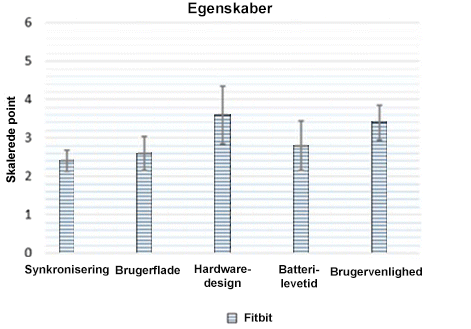
\includegraphics[width=0.7\textwidth]{figures/FeatureSatisfaction2}
	\caption{Grafisk repræsentation over tilfredsheden vedrørende Fitbit Flex' egenskaber; synkronisering, applikationens brugerflade, hardware design, batterilevetid og brugervenlighed \citep{kaewkannate2016}.}
	\label{fig:FeatureSatisfaction}
\end{figure}

\noindent
På \autoref{fig:FeatureSatisfaction} ses det, at Fitbit Flex' bedømmelse ligger mellem $2,4$ og $3,6$ på tilfredshedsskalaen anvendt i førnævnte studie. Dette betyder, at brugerne finder Fitbit Flex lettere anvendeligt og tilfredsstillende, hvad angår synkronisering, brugerflade og batterilevetid, mens det bedømmes som moderat anvendeligt og tilfredsstillende vedrørende hardwaredesign og brugervenlighed \citep{kaewkannate2016}.

\begin{figure}[H]
	\centering
	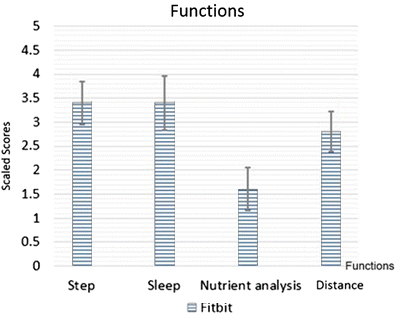
\includegraphics[width=0.65\textwidth]{figures/FunctionSatisfaction2}
	\caption{Sammenligning af tilfredshed vedrørende Fitbit Flex' funktioner \citep{kaewkannate2016}.}
	\label{fig:FunctionSatisfaction}
\end{figure}

\noindent
Funktionaliteten er bedømt på \autoref{fig:FunctionSatisfaction}. Her er Fitbit Flex bedømt mellem lettere og moderat anvendeligt og tilfredsstillende ved optælling af skridt, søvnmåling og afstandsmåling. Alle aktivitetsarmbånd i studiet blev bedømt som meget lidt til lettere anvendeligt og tilfredsstillende i forbindelse med næringsstofsanalyse \citep{kaewkannate2016}.

\subsection{Brugervenlighed}

Brugervenlighed er vigtig for, at teknologien anvendes korrekt, både for patienten og behandleren. Teknologien skal helst være nem at anvende, så der ikke opstår misforståelser i form af, hvordan teknologien anvendes, og hvordan resultaterne derfra tolkes. Yderligere er brugervenligheden essentiel for, at teknologien er let anvendelig, så det undgås, at teknologien er tidskrævende og besværlig for patienten at benytte \citep{Nordgren2013}. 

Brugervenligheden af Fitbit Flex bliver undersøgt i studiet af \citeauthor{kaewkannate2016}, hvor testpersonerne blev adspurgt, ved brug af en likert skala, hvorvidt de fandt Fitbit Flex let at anvende. På \autoref{fig:FeatureSatisfaction} i \autoref{sec:brugerbedommelse} kan det ses, at det gennemsnitlige svar fra testpersonerne ligger på omkring 3,5, hvilket på den anvendte likert skala i studiet, ligger mellem lettere og moderat tilfreds med brugervenligheden af Fitbit Flex \citep{kaewkannate2016}.

Studiet af \citeauthor{mercer2016}, der har testet forskellige aktivitetstrackere på kronisk syge personer over 50 år, har ligeledes med en likert skala spurgt testpersonerne, om de fandt aktivitetstrackerne lette at lære at anvende, forståelige og generelt nemme at anvende. Hertil er det gennemsnitlige svar ligeledes lidt over 3 på likertskalaen \citep{mercer2016}.

\subsection{Anvendelse af aktivitetstracker i hverdagen} \label{sec:anvendelse}

For at opnå forståelse for patientens oplevelse ved brug af aktivitetstrackere i hverdagen, tages der udgangspunkt i studier af \citeauthor{mercer2016} og \citeauthor{rapp2016}. Det førstnævnte studie undersøger implementeringen af aktivitetstrackere til motionsmonitorering af kronisk syge over $50$ år, hvor forsøgspersonerne tester en simpel skridttæller og fire aktivitetstrackere, for til sidst at bedømme forskellige aspekter ved anvendelse af disse. I det andet studie undersøges, hvordan forsøgspersoner uden tidligere erfaring med aktivitetstrackere oplever at måle deres aktivitetsniveau \citep{mercer2016, rapp2016}.

Forsøgspersonerne i \citeauthor{mercer2016} havde en gennemsnitsalder på $64$ år, hvor den yngste var $52$ og den ældste $84$, hvor alle var diagnosticeret med kroniske sygdomme, som blandt andet diabetes, vaskulære sygdomme eller gigt, hvorfor dette passer med den forventede målgruppe af patienter med hypertension. I studiet blev det fundet, at der var højere tilfredshed blandt forsøgspersonerne ved anvendelse af aktivitetstrackere frem for almindelige skridttællere, hvor skridttælleren i gennemsnit scorede $55,7$, mens aktivitetstrackerne scorede mellem $62,9$ og $67,6$ på en skala fra $0$ til $100$. Samtidig blev forskellige aspekter af brugertilfredsheden med aktivitetstrackerne og skridttælleren undersøgt, hvorigennem det blev fundet, at aktivitetstrackerne scorede højere i samtlige test vedrørende større opmærksomhed på egen aktivitet og brugervenlighed. Skridttælleren havde en fordel vedrørende tilkobling til anden teknologi, hvor de ældre manglede enhederne, som aktivitetsarmbåndene skulle kommunikere med ved dataanalyse, hvilket også er beskrevet i \autoref{sec:tek_fordelebegr} \citep{mercer2016}.

Førnævnte resultater giver en indikation om, at valget af aktivitetstracker ikke er lige så vigtig, som det er at give større mulighed for nem dataoverførsel og større indblik i data, der er relateret til aktivitetsmønsteret ved anvendelse af en aktivitetstracker frem for at indtaste data manuelt fra en skridttæller \citep{mercer2016}.

Af samme studie blev det fundet, at deltagerne mente, at brugen af aktivitetstrackere motiverede dem til mere aktivitet og gav større opmærksomhed omkring eget aktivitetsmønster. Patienterne blev samtidigt spurgt, hvorvidt de mente aktivitetstrackerne var sygdomsbehandlings- eller underholdningsteknologi, hvor størstedelen fandt det brugbart i sundhedsmæssige sammenhænge. I starten af studiet var forsøgspersoner, som ikke brugte smartphone eller tablet i hverdagen i tvivl om, hvorvidt de kunne deltage i studiet, men det blev fundet, at disse personer ofte havde færrest problemer med tilvænning ved brugen af ny teknologi. Størstedelen af problemerne opstod grundet manglende instruktioner til teknologien frem for anvendelse, når forsøgspersonerne først havde fået en forståelse for funktionen \citep{mercer2016}.

Den førnævnte motivationsfaktor bliver også nævnt i et studie af \citeauthor{rapp2016}, hvor et lignende aktivitetsarmbånd, Jawbone Up, blev båret i en længere periode ($10$ dage til $1$ måned). Her mener over halvdelen af de $14$ forsøgspersoner i alderen $19$ til $50$ år med et gennemsnit på $31,9$ år, at aktivitetsarmbåndet kan hjælpe til at forbedre aktivitetsvanerne under anvendelse. Her findes det også, at forsøgspersonerne stoppede med at anvende Jawbone armbåndet som følge af besværet ved upload af data, hvis dette ikke passede ind i deres livsstil. Samtidigt manglede forsøgspersonerne fastsatte mål, intuitive datarepræsentationer og opsummering af de målte data, for at motivationen til livsstilsændring blev konstant \citep{rapp2016}.

I \citeauthor{mercer2016} konkluderes, at den ældre del af målgruppen finder aktivitetstrackere mere motiverende end skridttællere, som følge af den forbedrede mulighed for at observere eget aktivitetsmønster mere detaljeret og nemmere, gennem digital overførsel af data, frem for manuel indtastning af resultater fra skridttællere. Samtidig er det også fundet, at en vigtig faktor i implementeringen er grundig instruering ved opstart af anvendelsen, så patienterne hurtigst muligt får et indblik i, hvordan aktivitstrackeren og brugerfladen i de tilhørende applikationer fungerer. Ud fra \citeauthor{rapp2016} findes det, at brugerflade, datarepræsentation og opstilling af nye mål har en betydning for motivationen til kontinuert ændring af livsstil, hvorfor fastsættelse af mål i samråd med lægen eller gennem den tilknyttede applikation potentielt kan forbedre brugeroplevelsen. Samtidig vil kombinationen af intet display på Fitbit Flex og interessen i egen aktivitet kunne bidrage til, at brugeren ofte vil synkronisere, for at følge med i den daglige fysiske aktivitet på smartphone eller computer.
\section{Patientens sociale og individuelle forhold i dagligdagen}
Idet en patient får tildelt et Fitbit Flex armbånd, er der forskellige tilhørende faktorer, der kan have betydning for patientens brug af armbåndet. 
Dette relaterer til, hvor avanceret teknologien er, og hvilke muligheder der er for at formidle den registrerede aktivitet for brugeren selv og omgangskreds. Dertil er det muligt at opdele disse faktorer i sociale og individuelle forhold, og kan være hæmmende eller motiverende for patienten.   

\subsection{Sociale forhold}
En implementering af Fitbit Flex til brug af patienter med hypertension, vil påvirke patienten og dennes sociale forhold. Fitbit Flex muliggør sammenligning med andre brugere af aktivitetsarmbånd over internettet, hvis patienten ønsker dette. Dette skaber en form for onlinefællesskab, hvor patienterne kan interagere med andre, der muligvis har lignende mål vedrørende daglig fysisk aktivitet \citep{karapanos2016}. 
Dette giver mulighed for, at patienten kan sammenligne sig med, og konkurrere mod, venner, kollegaer, familie, fremmede eller blot egne tidligere rekorder. På denne måde kan der skabes incitament til motion, hvis der konkurreres mod andre, da det kan virke som en motiverende faktor \citep{rooksby2014}.

I forhold til den valgte patientgruppe, kan alderen af patienten være afgørende, da prævalensen af hypertension stiger med alderen. I aldersgruppen $>50$ år har næsten $50~\%$ af befolkningen hypertension \citep{kronborg2008}. Denne aldersgruppe, især den ældste del af patienterne, vil ikke nødvendigvis kunne benytte sig af de sociale aspekter af aktivitetsarmbåndene, hvis de ikke er bekendte med sociale medier til dagligt. Disse vil udelukkende få gavn af de simple funktioner af et aktivitetsarmbånd, hvorfor det skal tages højde for, at alle patienter ikke vil få det samme udbytte af brugen af teknologien \citep{mercer2016}. Hvis de ældre patienter er i stand til at synkronisere sit armbånd, så familiemedlemmer vil kunne tilgå dennes data via internettet, vil dette muligvis kunne fungere som en motiverende faktor, hvis de er klar over, at familien følger med i deres aktivitetsniveau.

\subsection{Individuelle forhold}
I forhold til den valgte patientgruppe, kan der være nogle individuelle forhold, der afgør, om aktivitetsarmbåndet vil blive brugt af patienterne. Dette kan især være aldersgruppen af patienterne. 

Den ældre del af patientgruppen kan være tilbageholdende over for ny sundhedsteknologi, som de selv skal betjene, da dette kræver en indsigt i, hvordan denne slags teknologi fungerer. Ikke alle i aldersgruppen, $>50$ år, har meget erfaring med brug af denne type teknologi, hvilket kan gøre nogle patienter tilbageholdende fra at tage teknologien til sig, selvom den er relativt brugervenlig \citep{mercer2016}. 

I et studie af en gruppe af kronisk syge i alderen $>50$ år, som havde gået med aktivitetsarmbånd over en periode, ville $73~\%$ af studiets deltagere købe en aktivitetstracker, da de generelt var tilfredse med én eller flere af de afprøvede aktivitetstrackere. I dette studie lagde patienterne blandt andet vægt på, om den var behageligt at gå med, og om den var pæn, så den fungerede som en form for smykke \citep{mercer2016}.
\section{Effekter af monitorering af aktivitetsniveau}
%Indhold: I dette afsnit vil vi analysere effekter af en implementering af Fitbit Flex med hensigt på monitorering af aktivitetsniveau. Vi vil herunder komme ind på, hvilke effekter der er mulige at opnå, samt tidshorisonten på effekterne, om teknologien vil være en motiverende faktor for patienten til en mere aktiv hverdag, og om den kan være demotiverende, fx hvis der ikke sker en ændring. Vi vil se, om vi kan estimere, hvor stor en andel af patienter, der oplever en positiv virkning/effekt. 

Hypertensive patienters anvendelse af Fitbit Flex kan have forskellige virkninger på patienter og deres holdning til fysisk aktivitet, og det kan desuden påvirke forholdet mellem patient og læge.

Der er ikke fundet tal, der direkte viser sammenhængen mellem anvendelse af aktivitetsarmbånd og effekten af dette, så det er usikkert, hvor mange patienter, der reelt vil have en positiv effekt af anvendelse af Fitbit Flex. Ud fra forskellige studier kan det estimeres, hvordan patienter med hypertension vil påvirkes ved implementering af aktivitetsarmbånd som en del af behandlingen.

Der er en række studier, blandt andet studiet af \citeauthor{mercer2016}, som også nævnes i  \autoref{sec:anvendelse}, der indikerer, at brugen af aktivitetsarmbånd kan give motivation til en mere aktiv hverdag. Det nævnes i studiet, at anvendelsen af aktivitetsarmbåndet giver brugeren bevidsthed om egen sundhed og aktivitetsniveau, hvilket i nogle tilfælde kan medføre et øget aktivitetsniveau. 

Testpersonerne, der deltog i studiet, blev, ved anvendelse af en likert skala, spurgt om, hvorvidt de følte, at aktivitetsarmbånd hjalp dem med at blive mere aktive. Til dette bliver der i gennemsnit givet et neutralt svar, således at der hverken var uenighed eller enighed om, at aktivitetsarmbånd medførte øget aktivitetsniveau hos den enkelte \citep{mercer2016}. Det kan derfor antages, at halvdelen af testpersonerne har oplevet, at aktivitetsarmbånd havde en positiv effekt på deres aktivitetsniveau.

Studiet konkluderer, at der er potentiale i at anvende aktivitetsarmbånd til at forbedre kronikeres motionsvaner. Desuden nævnes det, at implementering af aktivitetsarmbånd i sundhedssektoren ville kunne forbedre relationen mellem patient og læge, da det kan hjælpe lægen med at give patienten et bedre indblik i og bedre vejledning om patientens fysiske sundhed og vigtigheden af det \citep{mercer2016}. 
Et studie af \citeauthor{nelson2016} har undersøgt sammenhængen mellem anvendelse af aktivitetsarmbånd og testpersonens følelse af empowerment, hvilket er en følelse af handleevne og kontrol over beslutninger, der påvirker deres helbred \citep{toennesen2005}.

I studiet konkluderes, at forskellige egenskaber, såsom muligheden for at være en del af et fællesskab via en app og den feedback aktivitetsarmbåndet giver, har en positiv indflydelse på brugerens følelse af empowerment. Det faktum, at testpersonerne blev monitoreret havde dog ingen virkning på følelsen af empowerment, hvilket ifølge studiet kan skyldes, at monitorering associeres med negative konsekvenser, såsom invasion af privatlivet.
Studiet finder ligeledes, at jo større en brugers følelse af empowerment er, des mere tilskyndes denne til at opnå sine opstillede mål. Det påpeges dog i studiet, at testpersonernes generelle engagement til at opnå opstillede mål, var lavere end det er set i andre studier. Dette kan skyldes, at testpersonerne i dette studie ikke fik opstillet generelle mål for deres fysiske aktivitet, hvorimod testpersoner i andre studier skulle forsøge at nå mål opstillet af eller i samarbejde med andre. 

%- Nogle folk er motiveret. Nogle føler selv at det hjælper på deres sundhed. Kan få folk til at engagere sig mere i at opnå opstillede mål (måske mål opstillet sammen med læge, så det ikke er helt egne mål).  antage, at det vil have positiv på nogle patienter. Kilder siger desuden at kun patienter der er ”motiveret” til det kommer i non-farmakologisk behandling. 

%\citep{nelson2016}: http://www.sciencedirect.com.zorac.aub.aau.dk/science/article/pii/S0747563216302369 

\section{Etiske problemstillinger}
%Indhold: I dette afsnit vil vi se på, om der er etiske problemstillinger ved, at lægen kan monitorere patientens aktivitetsniveau i hverdagen, og i så fald disse dilemmaer opstår heraf. Vi vil herunder drage paralleller til teknologier, hvor lignende problemstillinger opstår (fx hjemmeblodtryksmåler). 

Ved implementering af ny teknologi eller nye ideer i sundhedssektoren vil der ofte opstå etiske problemstillinger som skal adreseres. Der vil derfor i dette afsnit blive forsøgt belyst hvilke etiske problemstillinger, Fitbit Flex som aktivitets monitoreringsenhed, vil kunne skabe i sundhedsektoren.

Rapporten \author{patienthome2015} beskriver, at hvis monitoreringen bliver hyppig og meget tæt på, kan det for nogle patienter komme til at føles som overvågning. Det kan derfor blive et dilemma som man må tage op med patienten. Om vedkommende ønsker at modtage behandlingen, til trods for at der monitoreres kontinuert. I forhold til Fitbit Flex som monitorerer kontinuerlig aktivitet hos patienten, kan patienten selv tage stilling til om de ønsker behandlingen \citep{patienthome2015, SundhedsstyrelsenPatientersRetsstilling2016}.

Studiet af \author{Mittelstand2011} og \citep{Nordgren2013} har undersøgt en række etiske afspekter ved brugen af enheder der monitorerer patienten i privatlivet. Studierne understeger visse afpekter ved de etiske aspekter vedrørende monitorering af patienten i privatlivet.% Disse aspekter er, personlig privatliv og persondata, synlighed, medicinering, social issolation, aunonomi, pricip balance, informeret samtykke og udvikling, samt påvirkning på hjemmehjælpere. (jeg ved ikke helt om alle skal nævnes eller kun dem som er relevante for os, ordet aspekter bruges desuden ret meget :S) 
Af disse etiske aspekter vil Fitbit Flex primært kunne komme til at ramme områder som omhandler personlig privatliv og persondata, synlighed, autonomi, pålidelighed, brugervenlighed, helbred, samt uafhængighed \citep{Mittelstand2011, Nordgren2013}.

\noindent \\
\textbf{Privatliv og persondata:}
\noindent \\
Ved at patienten bliver monitoreret kontinuerligt i løbet af hele dagen, vil nogle brugere kunne komme til at se det som overvågnig som nævnt tidligere. Fitbit Flex kan følge patienters aktivitetsniveau i form af skridt og aktive timer, herved vil alle deres aktiviteter ikke kunne spores ned til mindste detalje da Fitbit Flex ikke inkluderer GPS, dog vil det stadig kunne give nogle spekulationer ved visse patienter muligvis....
Der kan stilles spørgsmålstegn til om data om fysisk aktivitet falder ind under kategorien over følsom persondata, om det kan misbruges på nogen måde. Dog vil det ikke være lige så følsomt som data der vedrører patienten direkte, så som CPR nummer eller andet som kan bruges til at identificere eller skade patienten \citep{Mittelstand2011}.

\noindent \\
\textbf{Synlighed:}
\noindent \\
Synlighed vedrører enhedens fysiske fremtræden, altså om enheden er stor, klodset og tung for patienten at gå med, så den  genere patienten i hverdagen. Fitbit Flex bæres som et andet armbåndsur og ses derfor ikke for generende for patienten, med mindre der er personlige ting som gør at de ikke kan gå med uret, for eksempel allergier eller andet. Yderligere kan det også overvejes at nogle patienter vil komme til at føle sig stigmatiseret, hvorved de kan gå i en tro om den overbevisning om at de er syge, teknologien kan være symbol for dette \citep{Mittelstand2011}. 

\noindent \\
\textbf{Autonomi:}
\noindent \\
Den behandling patienten modtager skal være forståelig og patienten skal være indbefattet med hvad behandlingen kommer til at betyde for vedkommendes liv. Introduktionen af teknologien for patienten er derfor vigtig. Hvis teknologien kan ændre på patientens daglige rutiner, vil patienten skulle tilpasse sig en ny livsstil, hvilket Fitbit Flex nemt kan komme til at gøre, da et af formålene med Fitbit Flex er at motivere patienterne til at være mere aktive. Denne omvendig kan være svær for nogen \citep{Mittelstand2011}. %... Selvbestemmelse...

\noindent \\
\textbf{Pålidelighed:}
\noindent \\
Pålidelighed spiller en rolle for at den dokumenterede aktivitet som Fitbit Flex registrerer kan gengive den aktivitet som patienten har udført præcist. Afhængig af behandlingen kan pålidelighed være vigtigere, for eksempel ved måling af blodglukoseniveau hos diabetikere. Hvis Fitbit Flex ikke viser patienternes fysiske aktivitet som den reelt er, eksempelvis ved at den har svært ved at registre visse former for aktivitet \autoref{xxx} kan behandlingen have en negativ effekt for forløbet... \citep{Nordgren2013}. Hvor godt Fitbit Flex repræcenterer fysisk aktivitet er beskrevet i afsnit \autoref{pålidelighedsafsnittet}.

\noindent \\
\textbf{Brugervenlighed:}
\noindent \\
Brugervenlighed er vigtig for at teknologiens anvendelse, både for patienten og behandleren. Teknologien skal helst være nem at anvende så der ikke opstår misforståelser mellem de parter som teknologien berører, samt for at mindske risikoen for at teknologien fylder for meget i patientens hverdag  \citep{Nordgren2013}. Brugervenlighed for Fitbit Flex beskrives i afsnit \autoref{brugervenlighed}.
 
\noindent \\
\textbf{Helbred:}
\noindent \\
Behandlingen som patienten modtager har til hensigt at gøre patientens helbredstilstand bedre, eller undgå at den bliver værre og ikke forværre den. Fitbit Flex har som aktivitetstracker, til formål at dokumentere den fysiske aktivitet patienterne udfører, samt motivere patienterne til at udføre mere aktivitet i hverdagen, ved at for eksempel at sætte mål for patienten \citep{Nordgren2013}. 

\noindent \\
\textbf{Uafhængighed:}
\noindent \\
Ved at patienterne modtager et Fitbit Flex, er det i den forventning om at de skal få en mere aktiv hverdag. Patienter er ikke tvunget til at fuldføre denne forventning, da teknologi ikke skal bestemme over patienternes aktiviteter og hvad de foretager sig. \citep{Nordgren2013}
\\

Et andet etisk aspekt ved patient monitorering er, hvem og hvor mange der skal have ejerskab og ansvar over den data som der bliver indsamlet, samt hvordan det undgås at drukne i datamængder. Data skal prioriteres så det kun er det data man kan bruge til den reele behandling som bliver "gemt", der skal derfor tages stilling til hvad der er vigtigt \citep{patienthome2015}. Eksempelvis vil data fra Fitbit Flex, som er relevant for lægen, de data som fortæller noget om hvor aktiv patienten er i hverdagen, altså data som aktive timer, skridt gået, samt forbrændte kalorier. Data som søvnovervågning eller andet aktivitetarmbåndet kan registere vil være overflødigt for formålet med aktivitetsarmbåndets brug i forhold til hypertension, da dette ikke giver nogen direkte indikation vedrørende patientens aktivitetsniveau. Data skal derfor begrænses så det tilpasses til det som er nødvendigt for patientens forløb. 

\\
Generelt er problematikken vedrørende de etikske aspekter ved Fitbit Flex lille sammenlignet med andre teknologier som indgår til behandling af patienter. \textbf{Tanken med dette var lidt at lave en slagt opsummering af det der er skrevet, ved ikke om det er nødvendlig, det er det måske ikke}

\\
\textbf{Det kan godt være at nogle af tingene enten skal beskrives bedre, på en anden måde, jeg er også lidt i tvivl om strukturen på dette afsnit... om der er for meget "gentagende" med eller bare for meget med. Nogle af sætningerne skal nok måske højest sandsynligt også lige formuleres lidt bedre :) }











%Privatliv
%Personlig privatliv og person data er ... spørgsmplet er om PHM ses på som personlig data som andet personlig data, graden af følsomhed

%Synlighed, 
%Størrelse og vægt på den benyttede PHM enhed. Er det noget som generer patienten i hverdagen, fordi den er tung og klundtet eller bare en af delene? 

%Medicinering, 
%monitorering skal ikke bare anvendes for monitoreringens skyld.. fordi man kan gør man det, sådan skal det ikke være

%Social issolation, 
%Der er mindre brug for plejepersonale, dette leder til mindre kontakt med patienterne, det kan evt. laves en løsning i at patienterne kan kommunikere sammen gennem monitoreringsenheden... noget noget...

%Autonomi, 
%Selvbestemmelse, monitoreringsenheden kan lave om på patienternes daglige rutiner, ændre på patienternes selvbestemmelse... Patienternes handlinger.

%Princip balance, 


%Informeret samtykke og udvikling, 
%Fuld forståelse af teknologeiens påvirkning for patienterne kan ikke forudsiges direkte da det ikke er blevet gjordt endnu.

%Påvirkning på hjemmehjælpere.
%Hjemmehjælperne får færre opgaver at tage sig af, da teknologien tager over, hvilket også betyder at patienterne oplever mindre personalekontakt, hvilket er nødvendigt for nogen..
\section{Delkonklusion}
Indhold: Dette afsnit vil indeholde en delkonklusion af denne del af MTV'en og dette kapitel, som forhåbentligt vil lede frem til en endelig konklusion i syntesen. 

%-------------Organisation-----------
\chapter{Organisation}
Dette kapitel omhandler de organisatoriske ændringer, der kan forekomme ved implementering af Fitbit Flex til monitorering af hypertensive patienters aktivitetsniveau i den almene praksis. Leavitts modificerede organisationsmodel, beskrevet i \autoref{sec:metode_org}, anvendes til at beskrive disse ændringer. I kapitlet undersøges tilrettelæggelse og opgavefordeling i den primære og sekundære sundhedssektor, som påvirkes ved implementeringen af Fitbit Flex. Det undersøges også, hvilke behov læger i den primære sektor og hypertensive patienter har for introduktion til teknologien i forbindelse med implementeringen.   


% Indhold i afsnittet
\section{Patientforløb med hypertension}
Tages der udgangspunkt i Leavitts modificerede organisationsmodel, er der en række variable i organisationen, der vil påvirkes, hvis der sker en organisationsforandring. Disse variable er henholdsvis struktur, teknologi, aktører, opgaver samt omgivelser, hvilket fremgår af \autoref{fig:leavittmodel} \citep{mtvhaandbog}.

Implementeres Fitbit Flex, som et led i behandlingen af hypertension, kan dette påvirke de resterende organisationsvariable i forskellige grader afhængig af, hvilken virkning teknologien har på behandlingsforløbet.

Aktørerne, læger eller sygeplejersker i almen praksis, vil få til opgave at lære at anvende aktivitetsarmbånd som en del af et behandlings- og monitoreringsforløb for hypertensive patienter. Indførelse af aktivitetsarmbånd kræver derfor, at de alment praktiserende læger ønsker at innovere behandlingen og anvende den alternative behandlingsmetode i klinikkerne. Nogle vil muligvis være skeptiske over for indførelse af en ny teknologi, såsom Fitbit Flex. De læger, der har interesse i at benytte aktivitetsamrbånd i form af Fitbit Flex, kan indføre det i praksis. Har indførelsen en positiv effekt, kan teknologien udvides til flere alment praktiserende klinikker, hvis disse ændrer mening.

For at gøre det mere attraktivt for de praktiserende læger at anvende en ny teknologi, der kræver omstilling i forhold til den almindelige arbejdsgang, kan der indføres et honorar for anvendelse af aktivitetsarmbånd som en del af behandlingen for hypertension. Ved at honorere anvendelse af nye teknologier i almen praksis, kan anvendelsen af udstyret øges, hvilket eksempelvis har gjort sig gældende ved hjemmeblodtryksmåling \citep{bang2006}.

\subsection{Diagnose og udredning af hypertension} \label{sec:dia_hypertension}

Hypertension giver sjældent symptomer og opdages derfor ofte ved en tilfældighed ved eksempelvis sundhedstjek hos patientens alment praktiserende læge. Diagnosen hypertension kan ikke stilles efter én måling foretaget hos lægen, da patienten kan være nervøs og derved have et højere blodtryk og påvirke resultatet. Patienten bør få foretaget enten døgnblodtryksmåling eller hjemmeblodtryksmåling, hvis målinger i klinikken viser forhøjet blodtryk. Patienten kan desuden sidde i et rum uden tilstedeværelse af sundhedspersonale og få foretaget blodtryksmålinger med en automatisk blodtryksmåler \citep{lodberg2016, bech2015}.

Viser flere blodtryksmålinger et forhøjet blodtryk skal patienten igennem en videre udredning. Patientens tidligere sygehistorie vil tages i betragtning, herunder blandt andet forskellige risikofaktorer for hypertension såsom lavt aktivitetsniveau, diabetes og familiær disposition til blandt andet hypertension, diabetes og nyresygdomme. Foruden dette foretages en objektiv undersøgelse af patienten, hvor blandt andet højde, vægt og abdominalomfang måles. Der tages desuden EKG-målinger, blodprøver og urinprøver, og hvis der er kliniske tegn på hjertesvigt, foretages røntgen af thorax og ekkokardiografi. Dette kan foregå i tilfælde, hvor patienten bliver henvist til sekundærsektoren \citep{lodberg2016, bech2015}.

Er den hypertensive patient under $40$ år, har et meget højt blodtryk eller har behandlingsresistent hypertension, bør patienten undersøges for sekundær hypertension for at sikre, at det ikke er en eller flere bagvedliggende sygdomme, der har hypertension som en følge\citep{lodberg2016}. Sekundær hypertension forekommer hos mindre end $5~\%$ af tilfældene, og den hyppigste årsag er nyresygdomme \citep{lodberg2008}. Patienten kan eksempelvis henvises til nefrologisk afdeling for yderligere undersøgelser, hvis der findes eller er mistanke om en bagvedliggende nyresygdom \citep{lodberg2016, sundhedsstyrelsen2010}. 

\subsubsection{Samspil mellem primær og sekundær sektor}
Under udredning og behandling kan hypertensive patienter, hvis nødvendigt, blive henvist til forskellige afdelinger af den alment praktiserende læge. Regionen, hvori patienten er bosat, har betydning for, hvor patienten henvises til. Henvisning kan eksempelvis være til Blodtrykscenteret i Region Midtjylland, hvor Nyremedicinsk, Hjertemedicinsk og Endokronologisk Afdeling i samarbejde behandler hypertension og eventuelle følgesygdomme eller sekundære årsager til hypertension. Patienter kan henvises til Blodtrykscenteret ved behandlingsresistent hypertension, hypertension i forbindelse med nogle former for hjertekarsygdomme, mistanke om sekundær hypertension, eller hvis nyopdaget hypertension skal verificeres ved hjælp af døgnblodtryksmåling. Ved en henvisning til Blodtrykscenteret vil patienten inden være forsøgt udredt af egen læge, hvor informationer om udredningen vedlægges  henvisningen \citep{aarhusuniversitetshospital}. 

I regioner uden et center lignende Blodtrykscenteret vil hypertensive patienter typisk blive henvist til nefrologisk, kardiologisk eller endokronologisk afdeling \citep{buur2011}. Når det vurderes af lægerne på den pågældende afdeling, at patienten har fået den tilstrækkelige behandling på afdelingen, afsluttes behandlingen, og patienten kan efterfølgende gå til kontrol ved alment praktiserende læge \citep{sundhedsstyrelsen2010, lodberg2016}.

Hvis Fitbit Flex bliver implementeret som en del af behandlingen af hypertension kan dette muligvis påvirke strukturen i organisationen ved at ændre antallet af patienter, der bliver henvist til forskellige afdelinger i den sekundære sektor. Hvis aktivitetsarmbåndet har en positiv effekt, og flere patienter får det bedre af at få et højere aktivitetsniveau, kan der muligvis være færre følgevirkninger såsom nyresygdomme og hjerteproblemer, og det vil derfor ikke være nødvendigt at henvise disse patienter til den sekundære sundhedssektor. 

\subsection{Behandling af hypertension}

Når den alment praktiserende læge har diagnosticeret og vurderet patienten, kan behandlingen påbegyndes. Behandling af hypertension afhænger af, hvilken grad af hypertension patienten har, samt hvorvidt det er sekundær hypertension. Det er herved forskelligt, hvor og hvem der varetager behandlingen. Opstår følgevirkninger, der kræver yderligere behandling, henvises patienten til en specialiseret afdeling, hvor behandlingen varetages, indtil patienten er stabil og kan fortsætte hypertensionskontrol hos egen læge \citep{sundhedsstyrelsen2010}.

Som skrevet i \autoref{sec:hypertension} har lægen i den almene klinik mulighed for at behandle hypertensive patienter farmakologisk og non-farmakologisk. Behandlingen vurderes ud fra, om patienten har risiko for kardiovaskulær sygdom, hvor lægen blandt andet undersøger om patienten har risikofaktorer såsom hypertensive organskader, diabetes og nyresygdomme \citep{promedicin2016}.

Farmakologisk antihypertensiva-behandling startes, hvis patienten har et blodtryk på over $180$/$105$ mmHg, da det på dette tidspunkt ikke er tilstrækkeligt med omlægning af livsstil, herunder rygestop, motion, kostændringer og saltindtag \citep{pedersen2016}. 

\begin{figure}[H]
\centering
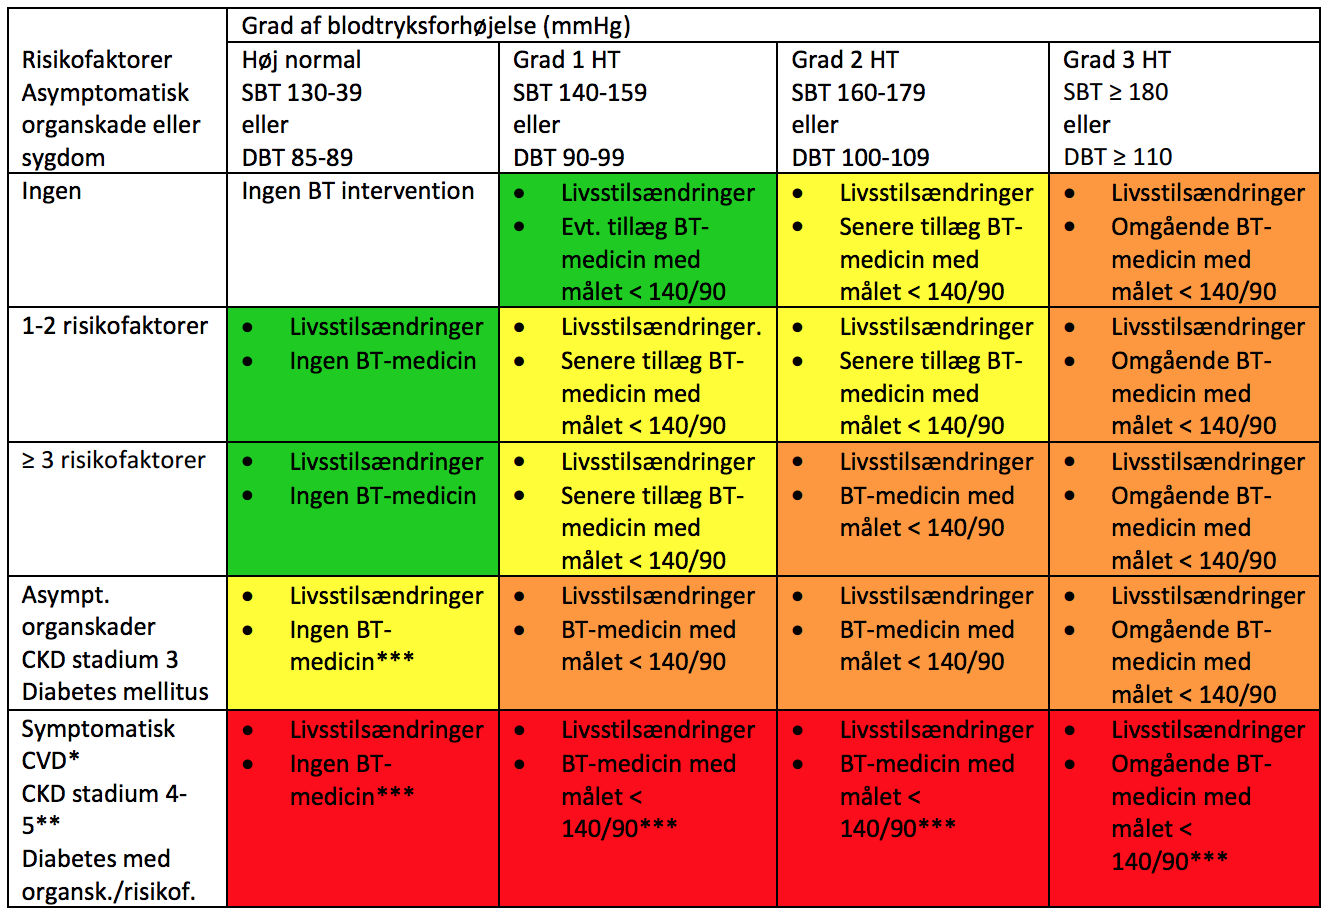
\includegraphics[width=0.9\textwidth]{figures/behandlingsvejl}
\caption{$10$ års risiko for apopleksi eller myokardieinfarkt. Rød: meget høj risiko ($>30~\%$), orange: høj risiko ($20-30~\%$), gul: middel risiko ($15-20~\%$) og grøn: lav risiko ($<15~\%$) samt hvilken konsekvens, som bør drages af inddelingen. (HT: hypertension; SBT: systolisk blodtryk; DBT: diastolisk blodtryk). *: CVD (kardiovaskulær sygdom), **: CKD (kronisk nyresygdom), ***: Evt. strammere blodtryksmål hos visse patienter med diabetes og patienter med proteinuri \citep{bech2015}.}
\label{fig:behandlingsvejl}
\end{figure}

\noindent
Mængden af forskellige farmakologiske præparater, patienten skal have, afhænger af de tidligere nævnte risikofaktorer, som lægen undersøger for, samt hvor forhøjet blodtrykket er. Dette fremgår af \autoref{fig:behandlingsvejl}. Har patienten en mild grad af hypertension, hvilket illustreres med grøn på \autoref{fig:behandlingsvejl}, kan patienten muligvis nøjes med livsstilsændringer, hvis der er få risikofaktorer. Ved middel til meget høj risiko for følgesygdomme af hypertension, illustreret med gul, orange og rød på \autoref{fig:behandlingsvejl}, bør der tillægges blodtryksmedicin \citep{bech2015}.
\citeauthor{munck2007}, som er et projekt ved Forskningsenheden for Almen Praksis i Odense, har udgivet en rapport omhandlende registreringer af hypertension i 184 almene praksisser. Ifølge denne rapport var $35,3~\%$ af de hypertensive patienter for lidt fysisk aktive, og for lavt aktivitetsniveau var dermed den tredje hyppigste risikofaktor \citep{munck2007}.

Ifølge \cite{munck2007} er $11~\%$ af de registrerede hypertensive patienter i non-farmakologisk behandling, samtidig er det kun $1,7~\%$ af de registrerede patienter, der ikke får nogle former for farmakologisk behandling \citep{munck2007}.
 %(Jeg ved ikke hvor jeg er på vej hen… Hjælp. Er alt det her overhovedet relevant at have med? DET ER COOLT MED TAL, HVOR MANGE DER EGENTLIG BLIVER BEHANDLER ALTSÅ HVOR MANGE DER ER REGISTRERET. JA JEG SYNTES OGSÅ AT DET VIRKER MEGET FORNUFTIGT)
Anvendelse af aktivitetsarmbånd til behandling af hypertension vil høre under kategorien non-farmakologisk behandling, hvor lægen eller sygeplejersken vil få arbejdsopgaver i form af at oplære patienten i brug af armbåndet og siden følge op på aktivitetsniveauet. Lægen kan ud fra data om aktivitetsniveauet vejlede patienten om motion. Skulle der ske en forhøjelse af blodtrykket under behandlingen, kan lægen kontrollere, om det kan skyldes et lavere aktivitetsniveau end normalt, eller om et lavere blodtryk kan skyldes, at aktivitetsniveauet er steget. Det vil på denne måde være muligt at sammenligne objektive målinger af aktivitetsniveauet med patientens prognose. 

\subsection{Aktivitetsarmbånd i den nuværende organisation}
Ifølge Leavitts modificerede organisationsmodel skal der tages højde for omgivelser, der påvirker samspillet mellem struktur, teknologi, aktører og opgaver. Ved omgivelser forstås en begrænset interessentanalyse \citep{mtvhaandbog}. Mulige interessenter for anvendelse af aktivitetsarmbånd som en del af behandling mod hypertension, er de praktisserende læger.

Ifølge \citeauthor{munck2007} blev der udsendt spørgeskemaer til de almene praksisser, der deltog i undersøgelsen. Spørgeskemaerne blev besvaret af en kontaktperson i hver praksis. Der blev blandt andet adspurgt om, hvorvidt det ønskes, at personale involveres mere i patientbehandlingen af hypertension, hvortil $67,3~\%$ svarede ja. Ud af disse svarede omkring $49~\%$, at de ønsker øget involvering indenfor vejledning om motion og fysisk aktivitet \citep{munck2007}. Disse tal kan tyde på, at en stor andel af de almene praksisser kan være åbne for nye muligheder eller forbedringer inden for vejledning om fysisk aktivitet i forbindelse med hypertension. Ved indførelse af Fitbit Flex som en del af behandlingen af hypertension har personalet i den almene praksis mulighed for at monitorere patientens fysiske aktivtetsmønster og kan dermed få bedre mulighed for at tilpasse vejledningen til patienten. 

Andre mulige interessenter kan også være læger og andet personale i den sekundære sektor. Blodtrykscenteret i Region Midtjylland reklamerer blandt andet med, at forskning og implementering af nye behandlingsmetoder foregår med udgangspunkt i Blodtrykscenteret \citep{aarhusuniversitetshospital}. Foruden dette kan afdelinger på sygehuse, der behandler mange hypertensive patienter, have interesse i at få implementeret behandlingen i de almene klinikker. Hvis antallet af svære tilfælde af hypertension formindskes, kan det dermed påvirke samspillet mellem primær og sekundær sektor. 
\section{Organisatoriske ændringer}\label{sec:org_aendringer}
Ved implementering af Fitbit Flex vil der forekomme ændringer i patientforløbet og i vidensbehovet for sundhedspersonale og patienter. 

Implementeringen vil påvirke patientforløbet, idet det skal vurderes, hvor i forløbet patienten skal introduceres for aktivitetsarmbåndet. 
Med udgangspunkt i \autoref{fig:patientforloeb}, anses det mest relevant at introducere patienten for og udlåne Fitbit Flex under behandlingsforløbet. Dette er vurderet ud fra, at patienten på daværende tidspunkt i patientforløbet vil blive givet en række anbefalinger, heriblandt fordelene ved fysisk aktivitet. 
Det anses ligeledes, at aktivitetsarmbåndet vil være fordelagtigt i relation til fremtidige kontroller, da dette vil give en indikation om, hvorvidt patientens aktivitetsniveau er stigende eller faldende fra forhenværende kontroller.   

Andre organisatoriske ændringer ses i relation til videnbehovet for at anvende teknologien i en medicinsk sammenhæng. Hertil skal både patient og læge have viden om teknologien. Det essentielle er, at både patient og læge skal være indforstået med, hvordan armbåndet bruges som et middel til dokumentation af patientens aktivitetsniveau. Hertil skal lægen vide, hvordan motion kan have en virkning på blodtrykket, og hvad det vil betyde for patienten, hvis vedkommende ikke er tilstrækkeligt aktiv i forhold til Sundhedsstyrelsens anbefalinger, som nævnt i \autoref{sec:prob_fysaktiv}. Sammenhængen mellem aktivitet og blodtryk er beskrevet i \autoref{sec:effekterafaktivitet}.

Lægen skal yderligere kunne vurdere, hvilke hypertensive patienter, der er egnet til at få et armbånd, hvorfor der i \autoref{sec:kriterier} opstilles forslag til patientkriterier for tildeling af et Fitbit Flex-aktivitetsarmbånd. I forlængelse med dette skal teknologien også tilpasses den enkelte patient, hvilket vil betyde, at lægen yderligere skal have færdigheder i brugertilpasning, som er beskrevet i \autoref{sec:brugertilpasning}. Lægen skal ved udlevering af Fitbit Flex kunne instruere patienten i brugen af armbåndet, samt de tilhørende dele og programmer, således patienten er i stand til at anvende armbåndets forskellige funktioner på egen hånd. \\

\noindent
Instruktionen af armbåndet vil som minimum skulle indeholde viden omkring: 
\begin{itemize}
\item Anskaffelse og installation af applikation på smartphone, computer eller lignende enhed
\item Hvordan armbåndet virker i forhold til, hvordan det registrerer fysisk aktivitet 
\item Brugerfladen af applikationen, samt hvordan patienten selv kan aflæse den registrerede fysiske aktivitet
\item Vigtigheden af jævnlig synkronisering af data , samt hvordan dette gøres
\item Hvordan batteriniveau aflæses, og hvordan batteriet genoplades \\
\end{itemize}


\noindent
Yderligere udleveres en brugermanual med armbåndet, som patienten kan anvende i tilfælde af tvivl eller spørgsmål. Det registrerede data skal efterfølgende også kunne aflæses af lægen, som derfor selv skal have indblik i brugerinterfacets funktioner.


 
\section{Efteruddannelse af personale}
\label{sec:efteruddannelse}
Når en ny teknologi indføres i den almene praksis, skal lægerne eller andet sundhedspersonale i praksissen lære at anvende teknologien, hvis den skal anvendes i et behandlingsforløb. 

Ifølge forskere indenfor læring og teknologiforståelse, som arbejder med forskningsprojektet Technucation, er forståelsen for teknologi vigtig i lægernes erfaring, da det er vigtigt at kunne se og forstå, hvordan teknologier anvendes og udnyttes på bedste vis \citep{aarhusuniversitet2013}. 

Herfor vil eventuel efteruddannelse kunne ses som relevant for lægerne i almen praksis, hvis et nyt redskab, som aktivitetsarmbånd til objektiv monitorering af patienters fysiske aktivitet, skal implementeres for at sikre, at de har en effekt i deres arbejde og, at de ydelser de medfører for patienterne lever op til forventningerne om at kunne monitorere patienternes fysiske aktivitet objektivt. Bogen \cite{hasse2012} beskriver teknologien på forskellige områder. Blandt andet beskrives teknologien som vigtig for at mindske fejl i systemet, da der for eksempel kan undgåes ulæselig håndskrift eller lignende ved anvendelse af teknologi. Ved at implementere aktivitetsarmbånd til monitorering af patienters daglige aktivitetsniveau, vil patienternes daglige fysiske aktivitetsniveau blive registreret på en mere objektiv måde end hvis patienterne selv skal fortælle om deres fysiske aktivitet, hvilket vil være mere subjektivt og derfor mindre troværdigt. Dokumentationen for patienternes fysiske aktivitet vil derfor være mere gyldig for at få et bedre overblik over patienten, hvis der anvendes objektive målemetoder \citep{hasse2012}. 

Efteruddannelsesfonden er etableret, så læger i den almene praksis, som deltager i efteruddannelse, har en konto, hvor lægen kan trække beløb fra til fravær, transport, kursusafgift og undervisningsmateriale. Denne konto er på cirka $13000$ kr. Dog skal bestemte kriterier være opfyldt for, at en læge kan få dækket udgifterne til efteruddannelse \citep{vedsted2005}. Et af disse kriterier er eksempelvis, at lægen skal arbejde efter overenskomst om almen praksis mellem Praktiserende lægers organisation (PLO) og Regionernes lønnings- og takstnævn (RLTN) \citep{fondenforalmenpraksis2016}. 

Efteruddannelse af læger kan passende foregå i samarbejde med de uddannelsesgrupper (tolvmandsforeninger), som ofte indgår i en læges netværk. Der vil i denne forbindelse kunne afholdes foredrag af en foredragsholder relateret til aktivitetsarmbånd og brugen i disse og hvordan de fungerer, for at lægerne får indsigt og uddannelse nødvendig for at kunne anvende dem til diagnosticering eller behandling af patienter \citep{vedsted2005}. 

\subsection{Analysering af data fra aktivitetsarmbånd}  
Data opsamlet fra aktivitetsarmbåndet skal analyseres med henblik på at se, inden for den periode patienten har gået med armbåndet, hvor meget patienten har været fysisk aktiv, og om denne fysiske aktivitet opfylder målene for at være aktiv nok.  

Med Fitbit Flex, som er yderligere beskrevet i \autoref{sec:teknologibeskrivelse}, vil den data, der er opsamlet blive overført ved at synkronisere enheden via en trådløs forbindelse, enten til smartphone eller PC, med bluetooth eller ved brug af den trådløse sync dongle, som følger med produktet. Denne synkronisering kan patienten foretage i eget hjem, hvorefter lægen kan se patientens data i klinikken ved at logge på patientens Fitbit bruger konto. Data, der opsamles, inkluderer blandt andet antal skridt gået, hvor lang en distance dette svarer til, antallet af kalorier forbrændt samt diverse grafer, som kan give patienten et overblik over, hvor meget den pågældende patient er aktiv. Dataene vil da kunne ses som tal eller grafisk ved hjælp af software programmet som hører til Fitbit \citep{fitbitflex}. 

Disse data vil kunne tastes ind i de databaser, som lægerne bruger, hvis dette er relevant for behandlingen af patienten eller som diagnosticerende middel. De data som lægen vil få fra aktivitetsarmbåndet vil være, antal skridt gået eller løbet, distancen, antal aktive timer, samt et estimat på kalorier forbrændt. Disse data vil skulle have en plads i lægens database, hvilket enten vil betyde at allerede anvendte programmer i den almene praksis skal tilpasses de nye data, eller der skal anvendes den allerede eksisterende platform fra fitbit, hvorved der vil skulle implementeres et nyt program i den almene praksis hvor aktivitetsarmbånd anvendes. 

\subsection{Indkøb af udstyr}	

Hvis aktivitetsarmbånd implementeres som en del af behandlingen af hypertension, skal det besluttes hvem, der har ansvar for anskaffelse af udstyret. Sundhedsvæsenet kan eksempelvis stå for indkøb af udstyr for at undgå, at patienten selv skal belastes økonomisk. 

Fitbit Flex kan købes over producentens egen hjemmeside, her er det muligt at forespørge om en større ordre via deres hjemmeside. Detailhandel kan derfor foregå for eventuelt at kunne spare penge ved at handle ind i et større parti af deres produkt.

Patienten kan eventuelt købe aktivitetsarmbånd billigere med en anbefaling fra lægen, eller få udleveret et aktivitetsarmbånd af lægen, som patienten beholder i et bestemt tidsinterval, eventuelt inden et kontrolbesøg hos lægen. Dette kan foregå ligesom ved udlevering af apparat til hjemmeblodtryksmåling, hvor patienten modtager klare instruktioner fra læge eller sygeplejerske inden brug og kan låne udstyret med hjem.

\subsection{Kontakt og information}

Problemer eller spørgsmål kan opstå enten fra læge til virksomheden, der producerer aktivitetsarmbåndet eller fra patient til læge. Herfor er det nødvendigt at kunne imødegå dette for at undgå, at der sker fejl eller misforståelser under forløbet, hvor patienten får målt deres fysiske aktivitetsniveau igennem hverdagen. 

\subsubsection{Mellem praktiserende afdeling/læge og producent}

Den praktiserende afdeling kan ved hjælp af producenten, Fitbits hjemmeside kontakte deres kundeservice på e-mail eller telefon, hvis der opstår problemer med produktet, eller hvis der er brug for at få en viden, som ikke kan findes "på egen hånd". 

\subsubsection{Mellem patient/borger og læge}

Hvis en patient efter at have fået udleveret et aktivitetsarmbånd bliver i tvivl om brugen af denne, vil det være nødvendigt for patienten at kunne kontakte lægen for yderligere information og vejledning. Ved at det er muligt for patienter at kontakte deres læge telefonisk kan mange misforståelser undgås og eventuel fejlbrug af udstyr. Lægen i den almene praksis skal som minimum have én time sat af til telefontid om dagen. Typisk er det i de sene morgentimer lægerne kan kontaktes telefonisk, dog kan der forekmme ventetider alt efter, hvor mange der prøver at komme i kontakt med den pågældende læge \citep{vedsted2005}. 

% kilde1 - Teknologiforståelse i sundhedsvæsnet (aarhusuniversitet2013)\\ 
% kilde2 - Almen praksis i Danmark (vedsted2005)
% En bog vi kan bruge "Teknologiforståelse på skoler og hospitaler", måske :) \\
% kilde3 - Teknologiforståelse på skoler og hospitaler (bog) (hasse2012)\\
% kilde4 - Fibit flex manual (fitbitflex)
% fondenforalmenpraksis2016: http://www.laeger.dk/portal/pls/portal/!PORTAL.wwpob_page.show?_docname=11221408.PDF

%Andre kilder som er værd at kigge på \\\\

%http://www.sst.dk/~/media/408300A6052D4D92BA02D486BD617613.ashx \\
%http://technucation.dk/laeringsaktivteter/laeringsaktivitet-ny-teknologi/ \\
%http://www.sst.dk/~/media/408300A6052D4D92BA02D486BD617613.ashx \\
%http://lvvl.dk/file/241981/vv12.pdf \\

%http://videnskab.dk/kultur-samfund/ny-teknologi-kan-skade-patienter-og-skoleelever-mere-end-den-gavner


\section{Delkonklusion}
Indhold: Dette afsnit vil indeholde en delkonklusion af denne del af MTV'en og dette kapitel, som vil lede frem til en endelig konklusion i syntesen. 

%-------------Økonomi----------------
%%%%%%%%%%%%%%%%%%%%%%%%%%%%%%%%%%%%%%%%%%%%%%%%%%%%%%%%
%\chapter{Økonomi}
%Dette afsnit omhandler det økonomiske aspekt ift. MTV analysen.
\chapter{Økonomi}

\section{Metode}
% Hvad koster den patientgruppe for samfundet? Hvad koster det, hvis de ikke passer deres sygdom ordentlig (i forhold til motion), og dermed får følgevirkninger (fx hospitalsophold, medicin)? (Cost/Benefit analyse??)
% Cost-effectiveness analysen (konsekvenserne måles i naturlige enheder)
%Cost-utility analysen (konsekvenserne måles i kvalitetsjusterede leveår (QALYs))
% Cost-benefit analysen (konsekvenserne opgøres i kroner og øre)
% Hvordan er omkostningerne sammenlignet med alternativerne?
% I forlængelse af, hvad aktivitetstrackeren skal kunne: Er de billige tilstrækkelige, eller er det nødvendigt at købe de dyre?
% Brugerbetaling eller egenbetaling??

I økonomianalysen undersøges hvilke omkostninger der er forbundet med anvendelse af aktivitetsmåler som dokumenteringsenhed for aktivitet i den almene praksis/medicin.
Ligeledes undersøges omkostninger for nuværende anvendelsesmetoder, samt hvilke økonomiske konsekvenser der forekommer når patienten ikke opretholder anbefalet aktivitetskvote.
Dette er med henblik på at fremhæve sundhedsgevinsterne i forhold til udgifterne.   
Omkostningerne og konsekvenser er opgjort af sundhedsøkonomiske analyser, som cost-effectiveness analyse (CEA), cost-utility analyse (CUA) og cost-benefit analyse (CBA), og oplyses i henholdsvis narturlige enheder (f.eks. vunde leveår), kvalitetsjusterede leveår og kroner øre. 
De estimerede værdier fra de forskellige analyser er baseret på eksisterende litteratur samt basale økonomiske udregninger.
Dette giver anledning til følgende MTV-spørgsmål: 

\subsection{MTV-spørgsmål}
%Eksempler
%\begin{itemize}
%\item Hvad vil forskellige modeller for vaccinationsprogram have af nytteeffekten i forhold til omkostninger?

%\item Hvordan ville en eventuel screening påvirke organisering og økonomi? 

%\item Hvad er de ressourcemæssige konsekvenser?
%\end{itemize}

\noindent  
\begin{itemize}
\item Hvad er omkostningerne ved nuværende anvendelsesmetoder, samt konsekvenserne ved utilstrækkelig aktivitetsydelse? 

\item Hvilke omkostninger er forbundet med brug af aktivitetsarmbånd til (?)-patienter, og hvad er den økonomiske konsekvens af dette, hvis brug af aktivitetsarmbånd resulterer i et øget antal kvalitetsjusterede leveår?

%\item Hvilke samfundsøkonomiske ændringer er der forbundet ved udlevering af aktivitetsmålere til patienter med ???.

%\item Hvordan ville et aktivitetsarmbånd påvirke organisering og økonomi?

%\item Hvilke omkostninger er forbundet med kvantificering af patientaktivitet, i forhold til nuværende anvendelsesmetoder (Aktivitetslog)?.  


\end{itemize}
 




% Indhold i afsnittet
%\section{Besvarelse}
Indhold: Dette afsnit vil indeholde forskellige underemner, der vil beskæftige sig med forskellige aspekter, så MTV-spørgsmålene kan besvares. 
\section{Nuværende omkostninger i sundhedssektoren}
Det er relevant at se på omkostningerne i sundhedssektorens primære og sekundære sektor ved brug af den nuværende målemetode. (RELEVANT IFT. HVAD?? JEG TROR DER MANGLER NOGET HER)

\subsection{Primær sektor} \label{sec:nuv_primaer}
\label{sec:primaer_sektor_omkostninger}
Den subjektive målemetode, der på nuværende tidspunkt benyttes af $27,7~\%$ af praktiserende læger, foregår ved spørgeskema under en konsultation, medfører udgifter i den primære sundhedssektor \citep{munck2007}. Afhængigt af antal konsultationer, som den enkelte kroniker har behov for, kan omkostningerne i forbindelse med konsultation ved udfyldelse af spørgeskemaer stige, mens udarbejdelse og udskrifter af spørgeskemaer vil have relativt lave omkostninger.
\citeauthor{munck2007} udarbejdede i 2007 en rapport om hypertension i almen praksis. Her blev $159$ kontaktpersoner i almen praksis spurgt: "Sætter I jeres hypertensionspatienter til kontrol med fast tidsinterval? Hvis ja, angiv det typiske interval" (MÅSKE MARKERE DETTE CITAT KURSIVT??). Her svarede $92,5~\%$, at de sætter deres patienter til kontrol med et fast tidsinterval, hvor den gennemsnitlige interval er udregnet til $3,9$ måneder \citep{munck2007}. 

Hvis det, jævnfør \citeauthor{kronborg2008}, antages at $1/5$ af den voksne danske befolkning har hypertension, vil dette svare til omkring $900.000$ danskere \citep{folketal2016}. Hvis $900.000$ danskere skal til lægekonsultation á $137,93$ kroner hver $3,9$. måned, vil dette svare til en årsomkostning for sundhedssektoren på omkring $380$ millioner kroner \citep{honorartabel2016}. 

Den samlede medicinudgift i den primære sundhedssektor i Danmark i $2014$ lå på $11,6$ milliarder kroner, og Danmarks Statistik påpeger i denne sammenhæng, at blodtrykssænkende medicin og hjertemedicin er nogle af de mest anvendte former for medicin i Danmark \citep{dst2016}. 

Ifølge en rapport udarbejdet af \citeauthor{apotekerforeningen2012} oplyses der, at de mest udleverede blodtrykssænkende lægemiddeler i år 2012, døgndosis (DDD) oplyses for hver, var amlodipin (139 DDD), furosemid (94 DDD), ramipril (92 DDD), bendroflumenthiazid og kalium (85 DDD), enalapril (80 DDD), samt losartan (73 DDD). Dette svarer til samlet $563$ millioner DDD i 2012 for disse blodtrykssænkende lægemidler for hele den danske befolkning \citep{apotekerforeningen2012}. DDD beskriver den anbefaldede dosis som patienterne skal have i forhold til prisen medicinen koster per dosis per dag. Hvis aktivitetsarmbånd som en non-farmakologisk  behandling implementeres i den almene praksis, vil der kunne spares på medicin DDD for patienter med hypertension, såfremt implementeringen påvirker patienternes helbred positivt. Ud over besparelser på DDD vil bivirkninger ved lægemidlerne også kunne reduceres, hvilket vil resultere i bedre livskvalitet for patienterne, samt et lettere behandlingsforløb. Eksempler på de hyppigste bivirkningerne ved de fleste af de nævnte lægemidler (ER DET HYPIGSTE BIVIRKNINGER VED DE NÆVNTE LÆGEMIDLER?? HVAD ER "DE FLESTE AF DE NÆVNTE") er ødemer, dehydrering, træthed, hovedpine og svimmelhed. Den bedste medicinering mod hypertension er individuel, hvorfor det ofte er nødvendigt at finde de lægepræparater, der er mest effektive for den enkelte patient, uden at der er for mange bivirkninger, hvilket besværligør og forlænger patienternes behandling.

\subsection{Sekundær sektor}
Den sekundære sektor påvirkes også af hypertension, da sygdommen er skyld i ambulante besøg og indlæggelser. I $2014$ var der $49.875$ ambulante besøg i den offentlige sekundære sektor for patienter med diagnosen blodtryksforhøjelse af enten kendt eller ukendt årsag, hvilket svarer til en stigning på $8,35~\%$ siden $2012$, hvilket kan ses på \autoref{fig:hyp_sekundaer} \citep{sundhedsdatastyrelsen2016}. 

\begin{figure}[H]
\centering
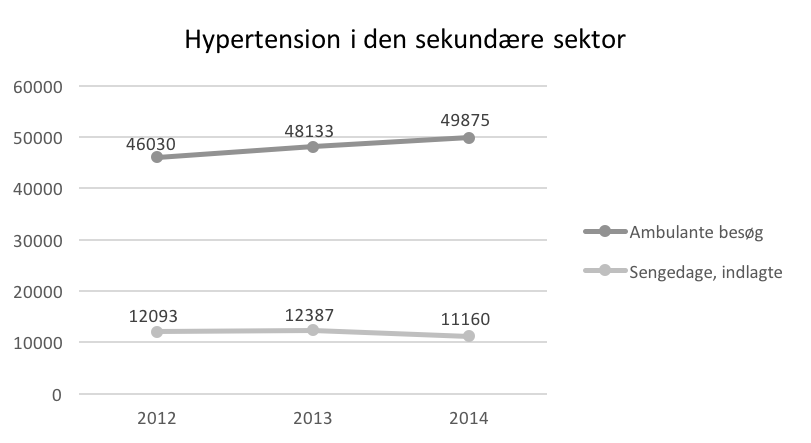
\includegraphics[width=0.8\textwidth]{figures/hyp_sekundaer}
\caption{Henvendelser i den offentlige sekundære sektor som følge af hypertension fra 2012 til 2014 \citep{sundhedsdatastyrelsen2016}.}
\label{fig:hyp_sekundaer}
\end{figure}

\noindent
Yderligere havde patienter med hypertension $11.160$ sengedage i forbindelse med indlæggelse på offentlige sygehuse i $2014$, hvilket var et fald i forholdt til de to foregående år \citep{sundhedsdatastyrelsen2016}. 

Jævnfør \citeauthor{takstvejledning2016} er taksten for et ambulant besøg  med journaloptagelse $1.421$ kroner uden nogen særlige procedurer, og taksten for en indlæggelse af en patient med hypertension er $12.597$ kroner indtil fire dage, der er det maksimale antal sengedage, der er dækket af denne takst. Ud over fire dage kan der opkræves en brugerbetaling for langliggertakst på $1.976$ kroner \citep{takstvejledning2016}. 

Hvis det antages, at ambulante besøg og antal sengedage i $2014$ er tilsvarende til henvendelser i år $2016$, så vil prisen for dette være omkring $210$ millioner kroner for ét år. 
\section{Omkostninger ved implementering af Fitbit Flex} \label{sec:armbaand_omkost}

Implementering af Fitbit Flex til patienter, som lider af hypertension, vil kunne medføre og antageligvis ændre de økonomiske udgifter i både den primære og sekundære sundhedssektor. I den primære sundhedssektor, som består af de praktiserende læger som behandlere, er det relevant at belyse de direkte omkostninger, der vil kunne forekomme i forbindelse med indkøb og implementering af teknologien, samt de indirekte omkostninger i form af, hvordan både den primære og sekundære sektor påvirkes i tilfælde af, at teknologien har en gavnlig effekt for patienterne. Hertil skal det overvejes, om teknologien skal være betalt af det offentlige, eller om den skal være brugerbetalt. 

\subsection{Direkte omkostninger} \label{sec:dir_omkost}
De direkte omkostninger er alle  udgifter, som relaterer til teknologien for eksempel ved indkøb af Fitbit Flex, implementering og brug i den almene praksis.  
Indkøbsprisen for et Fitbit Flex-armbånd er $749$ kr. hvis det købes gennem producentens hjemmeside. Dette beløb dækker over de omkostninger, der vil være tilknyttet til privat køb. 
Ved køb gennem sundhedssektoren betragtes dette som et virksomhedskøb, hvortil der ikke pålægges momsafgifter, hvilket udgør $20~\%$ af den opgivne pris. 
Der kan eventuelt indgås købsforhandlinger hos producenten, hvortil aftale om yderligere besparelse kan besluttes ved køb af større parti af produktet. Hvis produktet købes gennem sundhedssektoren, vil betaling af produktet med offentlig økonomisk støtte være mest hensigtsmæssig, da udstyret antageligvis kun vil blive udlånt til patienterne i over en periode og derefter leveret tilbage, hvorefter det kan genbruges af andre patienter. Det kan være fordelagtigt at indføre en testperiode, hvor en praksis indkøber et parti af produktet og efterfølgende følger op på patienterne før, der købes et endeligt antal af produktet for at sikre effekten. 

Udgifter, der kan være forbundet med en implementering, er efteruddannelse af personale som teknologien kommer til at berøre. Efteruddannelsesfonden stiller årligt $13.000$ kr. til rådighed \citep{vedsted2005}. Efteruddannelse af personale beskrives ligeledes i \autoref{sec:efteruddannelse}.   
Ved anvendelse af Fitbit Flex vil der opstå udgifter, der relaterer sig til udlån og introduktion af aktivitetsarmbåndet til patienterne. Til at bedømme omkostningerne forbundet ved brug af Fitbit Flex, tages der udgangspunkt i honorartabellen fra PLO \citep{honorartabel2016}. Tabellen er et opslag over, hvilke honorarer der kan gives praktiserende læger ved forskellige ydelser.
Da der ikke forekommer nogle direkte omkostninger i forhold til udlån og introduktion af aktivitets armbånd, sammenlignes der i stedet med udgifterne ved hjemmeblodtryksmåling. Udlevering af og introduktion til udstyr til hjemmeblodtryksmåling vil typisk forekomme ved en konsultation, hvorfor der også vil blive lagt honorar til dette. Honoraret for en konsultation ligger på $137,83$ kr. som tidligere nævnt i \autoref{sec:nuv_primaer}. Udlån og instruktion af hjemmeblodtryksmåler har et honorar på $141,68$ kr. hvilket vurderes at være sammenligneligt med et aktivitetsarmbånd, da det cirka omfatter de samme procedurer, dette kan eventuelt forekomme flere gange efter behov hos patienterne. Dette er et samlet honorar på $279,51$ kr. Hvis patienten bliver i tvivl om brugen af aktivitetsarmbåndet eller har flere spørgsmål, vil en telefonkonsultation være relevant at medtage; honoraret per telefonkonsultation er på $26,99$ kr.

\subsection{Indirekte omkostninger} \label{sec:indir_omkost}
De indirekte omkostninger vil typisk være de omkostninger, som er relateret til medicinforbrug, adminstration, samt forbedringer ved patienternes helbred som resultat af teknologien. 
Som det fremgår af \autoref{sec:primaer_sektor_omkostninger} udleveres $563$ milioner DDD af det mest populære blodtrykssænkende medicin fra apoteket. Hvis implementeringen af aktivitetsarmbånd har en positiv virkning på patienternes helbred, og dermed blodtryk, i og med, at de dyrker mere motion og får en sundere livsstil, vil der kunne skæres ned på behovet for medicin nødvendig for at behandle patienterne. Omkostningerne for disse DDD, vil dermed også kunne reduceres. Yderligere vil bivirkninger ved medicinen reduceres, hvilket vil øge patienternes livskvalitet, lette presset for behandlerne og forebygge bivirkningsrelaterede indlæggelser. 
Videresendelser af hypertensive patienter til den sekundære sektor vil ligeledes kunne blive reduceret, hvorfor patienterne kan forblive i et forløb som kun vedrører den primære sundhedssektor.   %\textbf{Det bliver lidt "punktet", det skal måske lige omformuleres lidt så der kommer et bedre flow i teksten :) }

\begin{comment}
Hvad koster et Fitbit Flex? 
Hvilke besparelser tilbydes der så sundhedsektoren? 

Hvad koster det så at introducere patienterne til teknologien? 
	Hvad dækker den her introduktion minimum over, for at kunne anvende armbåndet? (Anvendelse af app og hvordan den skal oplades.)
	
Hvad koster det hvis de har spørgsmål vedr. teknologien? 


%Diskussion orienteret 
Langsigtet omkostninger - hvis behandlingen hjælper/ikke hjælper
- Besparelser vedr. medicinering 
- Besparelser vedr. ambulant forløb 
- Forebyggelse af behandlingsresistent hypertension = $$$$



EVT: Dags-takster i sekundær sektor (Ambulant).



En model i almen praktsis for implementeringen af aktivitetsarmbånd?

Honorartabel = \citep{honorartabel2016}
\end{comment}
\subsection{Omkostninger i sundhedssektoren}
% har kombineret primær og sekundær sundhedssektor - gav ikke mening at adskille.. 

%Indhold: I dette afsnit vil vi gerne analysere og belyse mulige udgifter/besparelser ift. et muligt antal (reducerede) henvendelser til almen praksis ved benyttelse af ny teknologi, hvis dette er muligt at estimere. Herunder vil vi se på, om man vil kunne "nøjes" med telefonsamtaler eller emails for nogle af kontrollerne i stedet for egentlige konsultationer. 

%Indhold: I dette afsnit vil vi gerne analysere og belyse udgifter/besparelser ift. et muligt antal (reducerede) hospitalsindlæggelser ved benyttelse af ny teknologi, hvis dette er muligt at estimere.

Ved en implementering af Fitbit Flex, vil dette medføre ændringer i strukturen af den primære og sekundære sundhedssektor, som nævnt i \autoref{sec:org_aendringer}, hvor nogle mulige organisatoriske ændringer er beskrevet. Med de organisatoriske ændringer, vil der ligeledes følge ændringer i udgifter til sundhedssektoren. 
Håbet ved en implementering af Fitbit Flex er, at den vil medføre færre, økonomisk tunge, henvendelser til det offentlige. 

I den primære sektor, vil dette kunne ske, hvis antallet af blodtrykskontroller faldt. Dette kunne eksempelvis ske, hvis nogle fysiske kontroller erstattedes med telefoniske konsultationer, da honoraret for en telefonisk konsultation er 110 kroner lavere end en fysisk konsultation. Ud over denne økonomiske gevinst, skal der tages højde for, at der vil kunne være et øget antal henvendelser til egen læge i forbindelse med vurdering af patientens egnethed til brug af Fitbit Flex, udlevering og instruktioner i brugen af aktivitetsarmbåndet. 
 
Ligeledes vil der muligvis kunne være økonomiske besparelser, hvis en øget mængde fysisk aktivitet vil kunne reducere mængden af henvendelser til den sekundære sundhedssektor. Dette er muligt, da et ambulant besøg er 1.283 kroner dyrere end en konsultation, eller 1.394 kroner dyrere end en telefonisk konsultation ved egen læge. Hvis antallet af hospitalsindlæggelser endvidere kan mindskes, vil udgifterne dertil falde med 12.597 kroner per dag, det ikke er nødvendigt ikke at indlægge en patient. 

Regionerne

På denne måde, vil der kunne følge besparelser med en implementering af Fitbit Flex, der muligvis vil kunne udligne udgifterne til implementeringen af aktivitetsarmbåndet, som nævnt i \autoref{sec:armbaand_omkost}. 

Økonomi-afsnittet bliver nok primært spekulativt, da der er mange faktorer, som kan være voldsomt svære at estimere, men jeg synes, der er nogle fine betragtninger med. Tænk specielt over, at det godt kan være, at man har øgede omkostninger forbundet med armbåndet i primærsektoren, men at det man sparer i sekundærsektoren og i medicinudgifter opvejer dette på samfundsniveau. Det kan jo også være, at konklusionen simpelthen er, at det er for dyrt i forhold til gevinsten. En hård økonomisk konklusion kan nok være svær at nå til.
\section{Delkonklusion}
Indhold: Dette afsnit vil indeholde en delkonklusion af denne del af MTV'en og dette kapitel, som forhåbentligt vil lede frem til en endelig konklusion i syntesen. 

%-------------Syntese--------------------
\part{ Syntese}
%\chapter{Syntese}
\section{Diskussion}
\chapter{Konklusion}

Som konklusion på MTV'en besvares projektets problemformulering:

~
\begin{center}
\textit{Hvilke påvirkninger vil implementeringen af Fitbit Flex i den almene praksis til registrering og objektivisering af fysisk aktivitet have hos hypertensive patienter i sundhedssektoren?}
\end{center}
~

\noindent I MTV-analysen er det fundet, at brugen af Fitbit Flex i den primære sektor, vil give de praktiserende læger et mere objektivt grundlag for vurdering af hypertensive patienters aktivitetsniveau. Sammenlignet med den nuværende metode, hvor der primært anvendes spørgeskemaer, vil implementeringen af Fitbit Flex resultere i, at eventuel bias ved vurderingen af aktivitetsmønstret forsvinder som følge af, at patienternes aktivitet kvantificeres.

På baggrund af de undersøgte studier kan det påvises, at anvendelsen af aktivitetsarmbånd har potentialet til at resultere i en mere aktiv hverdag, som følge af den motiverende faktor i forbindelse med en forøget indsigt i eget aktivitetsmønster. Ud fra dette kan det konkluderes, at implementeringen af Fitbit Flex kan have en positiv indvirkning på hypertensive patienters aktivitetsniveau, hvilket kan forbedre patienternes tilstand, men dette kræver yderligere undersøgelser.

Ved implementering af Fitbit Flex vil patientforløbet og antallet af videresendelser fra primær til sekundær sektor kunne påvirkes. Dette sker som følge af, at patienterne har mulighed for at opnå en sundere livsstil ved anvendelse af armbåndet, hvorfor færre vil opleve en forværring af den hypertensive tilstand. Derved er det en mulighed at holde dem i den primære sektor, hvor der anvendes livsstilsændringer og blodtryksmedicin uden indlæggelser til behandling af sygdommen. Implementeringen vil påvirke den primære sektor i form af efteruddannelse til de indblandede parter, der skal udlevere armbåndet og instruere patienter i anvendelsen af teknologien.

Trods den motiverende faktor, som giver mulighed for et forhøjet aktivitetsniveau, vil Fitbit Flex ikke være et alternativ til anden behandling. Aktivitetsarmbåndet vil i stedet fungere som et hjælpemiddel til både læger og patienter, hvor det giver bedre vurderingsgrundlag og potentiale til sundere livsstil, som vil kunne betyde, at færre patienter videresendes ved forværring af hypertension.
\chapter{Anbefalinger}
Indhold: Dette afsnit kan indeholde nogle anbefalinger, hvis rapportens konklusion ender med at lede frem til nogle.

%-------------Bibliografi--------------------

\begingroup \label{litteratur}
\raggedright
\bibliographystyle{bibliography/unsrtnat}
\bibliography{bibliography/bibliography}
\endgroup


%-------------Bilag-------------------------
\begin{appendices}
%\chapter{Søgeprotokol}\label{app:soegeprotokol}
Indhold: Dette appendiks vil indeholde søgeprotokol for rapportens forskellige afsnit. Dette sættes ind, når søgningerne er udført. 
\end{appendices}



\end{document}